\documentclass[11pt]{article}
\usepackage[margin=1in]{geometry}
\usepackage{amsmath, amssymb}
\usepackage{graphicx}
\usepackage{float}
\usepackage{booktabs}
\usepackage[font=small,labelfont=bf]{caption}
\usepackage{subcaption}
\usepackage{xcolor}
\usepackage{enumitem}
\usepackage{hyperref}
\usepackage{multirow}
\hypersetup{colorlinks=true,linkcolor=blue!60!black,urlcolor=blue!60!black}

\title{\Large\textbf{GAD vs Sella on HIP --- T1x \emph{test} split, comprehensive}\\[4pt]
\normalsize 2026-04-29. Test split (n=287), 6 noise levels (10–200 pm),
threshold sensitivity, RMSD distributions, dt grid, IRC validation.}
\author{}
\date{}

\begin{document}
\maketitle
\thispagestyle{empty}

% =================================================================
\section*{🎯 Executive summary (added 2026-05-01)}
% =================================================================

\textbf{One-sentence headline.} \emph{When the Hessian is provided by an
ML interatomic potential (HIP), Gentlest-Ascent Dynamics outperforms the
P-RFO + quasi-Newton baseline (Sella) on chemistry-validated TS recovery,
with a margin that grows with TS-noise: tied below 50\,pm, $+$5.9pp at
100\,pm, $+$11.9pp at 150\,pm, $+$21.3pp at 200\,pm} (test split, n=287,
IRC TOPO-intended metric). Sella loses 4pp from raw conv to IRC-validated
because of \emph{wrong-saddle} failures; GAD loses 0pp.

\begin{figure}[H]
\centering
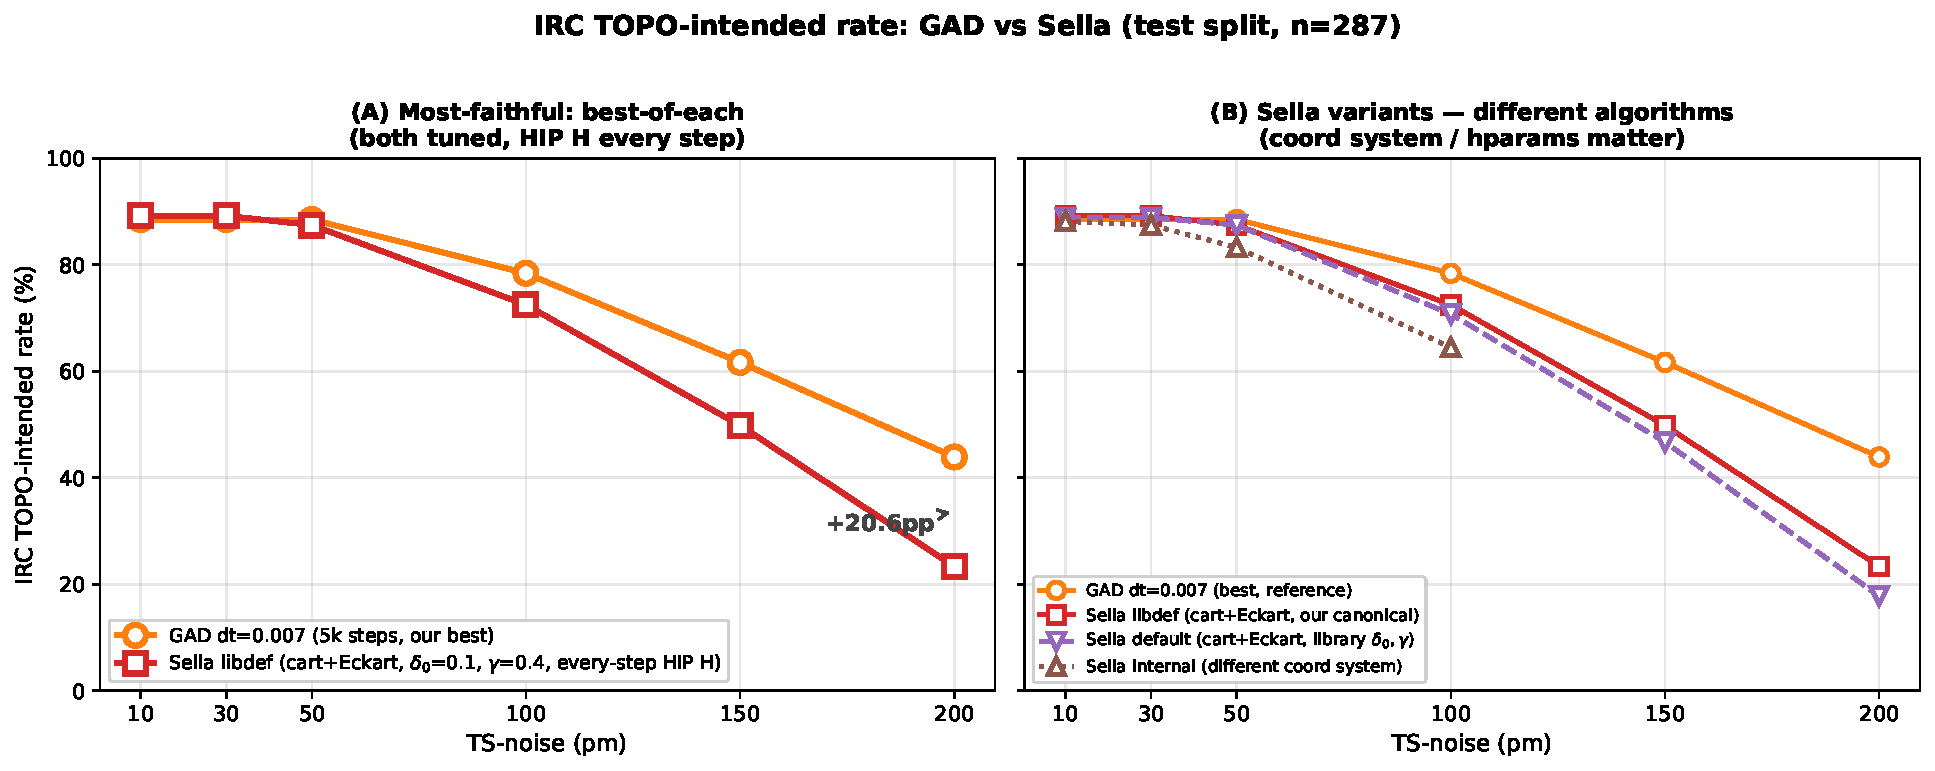
\includegraphics[width=\textwidth]{figures/fig_narrative_irc.pdf}
\caption{(A) The simple comparison: best-of-each, both tuned, both with
HIP H every step, same coord system, same step budget — the
``most-faithful'' framing. (B) Sella's variants are different
algorithms. We never collapse them under one ``Sella'' row;
internal-coords Sella is a different optimizer from Cartesian, etc.}
\label{fig:narrative-irc}
\end{figure}

\begin{figure}[H]
\centering
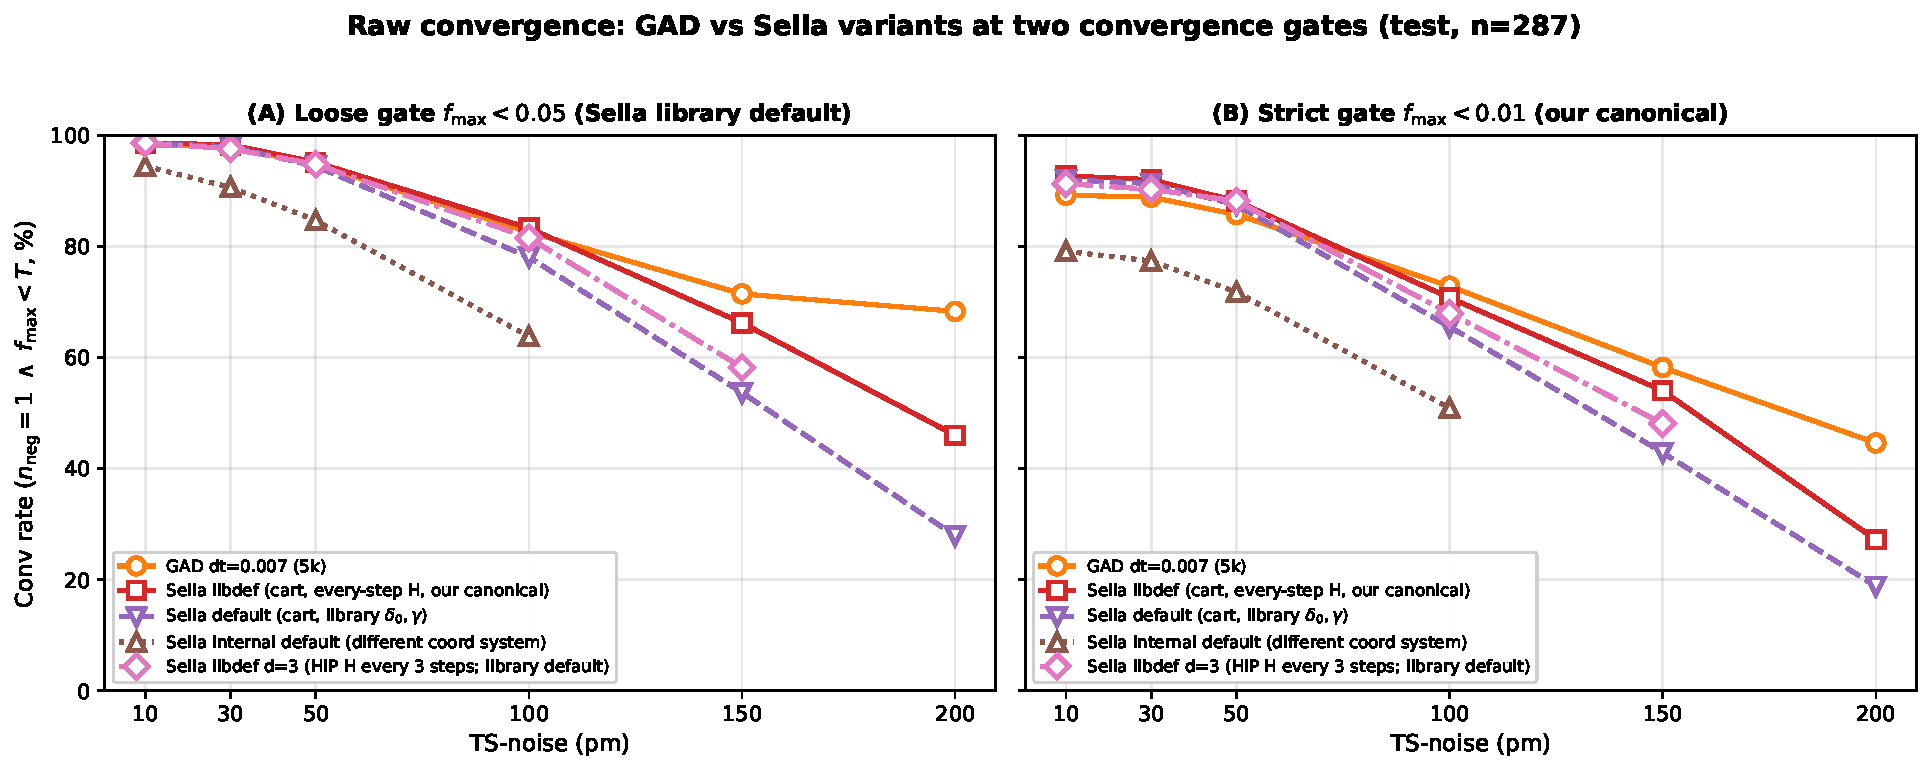
\includegraphics[width=\textwidth]{figures/fig_narrative_conv.pdf}
\caption{Raw-convergence companion (Sella's library default criterion fmax<0.05
left, our canonical fmax<0.01 right). At fmax<0.05 GAD wins by +22pp at
200pm; at fmax<0.01 by +17pp. IRC TOPO is the \emph{paper headline},
raw conv is supplementary.}
\label{fig:narrative-conv}
\end{figure}

\begin{figure}[H]
\centering
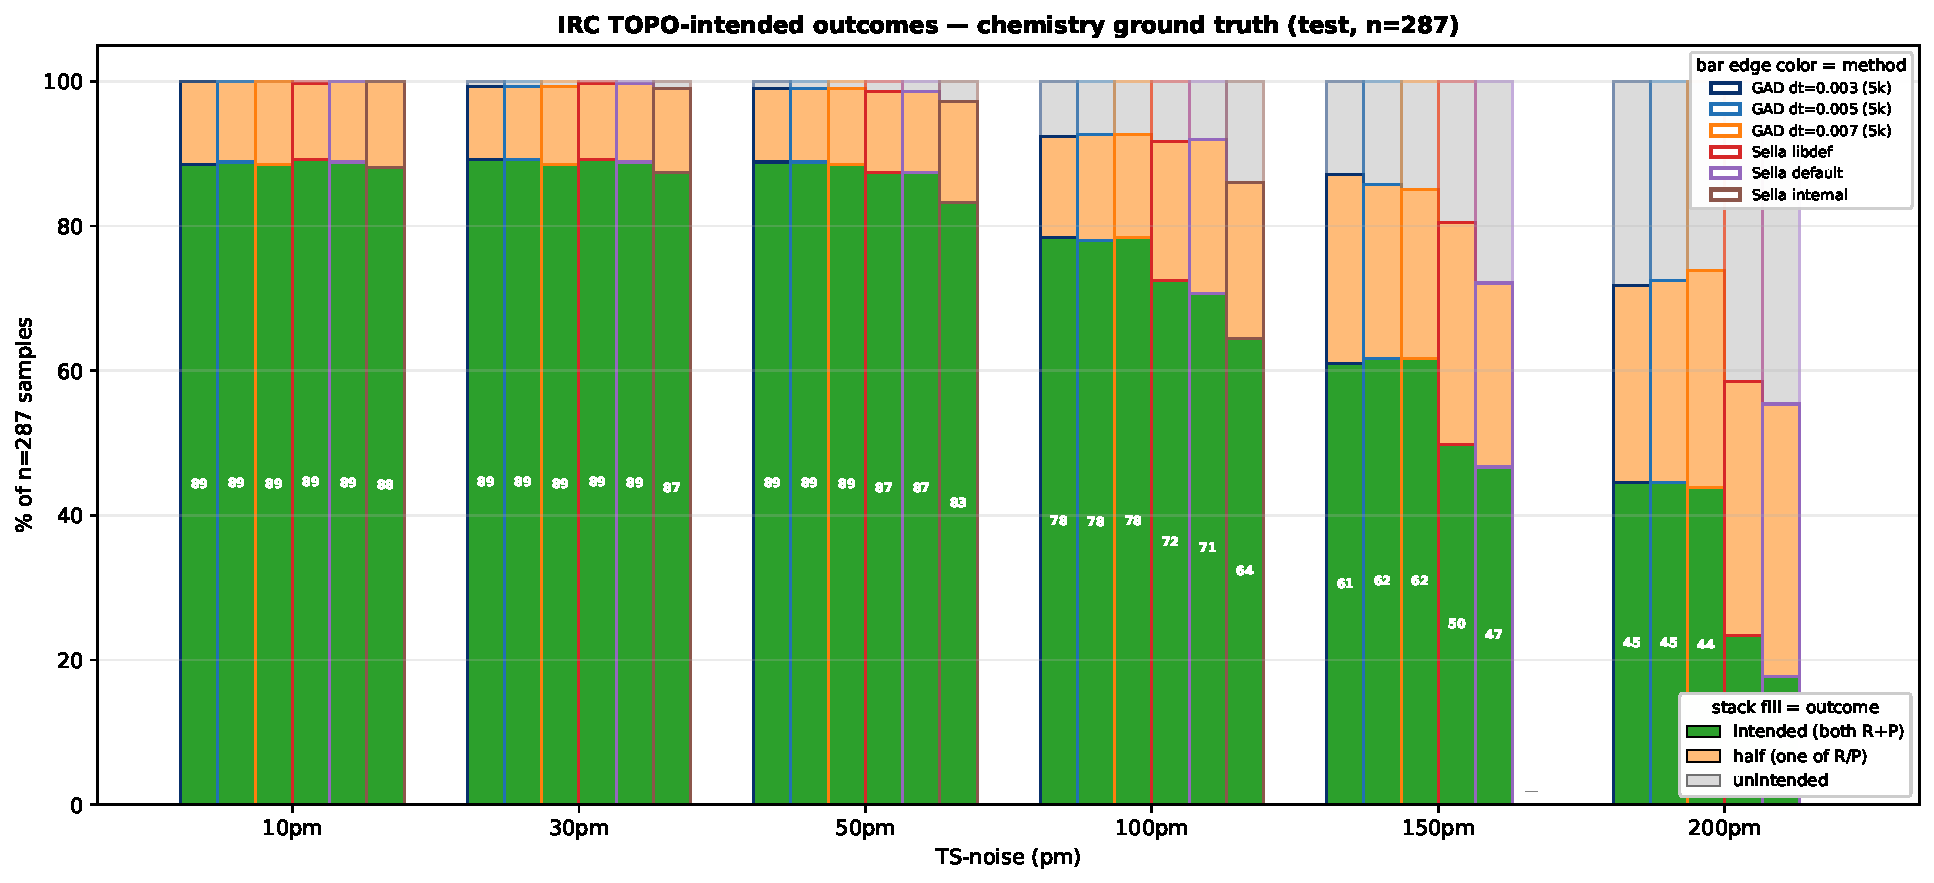
\includegraphics[width=\textwidth]{figures/fig_irc_bars_topo.pdf}
\caption{IRC TOPO outcomes per (method, noise) — \textbf{partitioned bars}.
Each bar = one method $\times$ one noise level, height = 100\% of $n=287$.
Green = both IRC endpoints match labeled R+P by element-aware bond-graph
isomorphism (the ``intended'' rate); peach = one endpoint matches;
gray = neither. \textbf{Green segment height is what we report as
TOPO-intended.} GAD's green stays at $\sim$45\% even at 200pm; Sella's
collapses to $<$25\%, with the loss going partly into ``half'' (one
endpoint OK) and ``unintended'' (wrong-saddle failures). Bar edge color
encodes method (legend top right).}
\label{fig:irc-bars-topo}
\end{figure}

\begin{figure}[H]
\centering
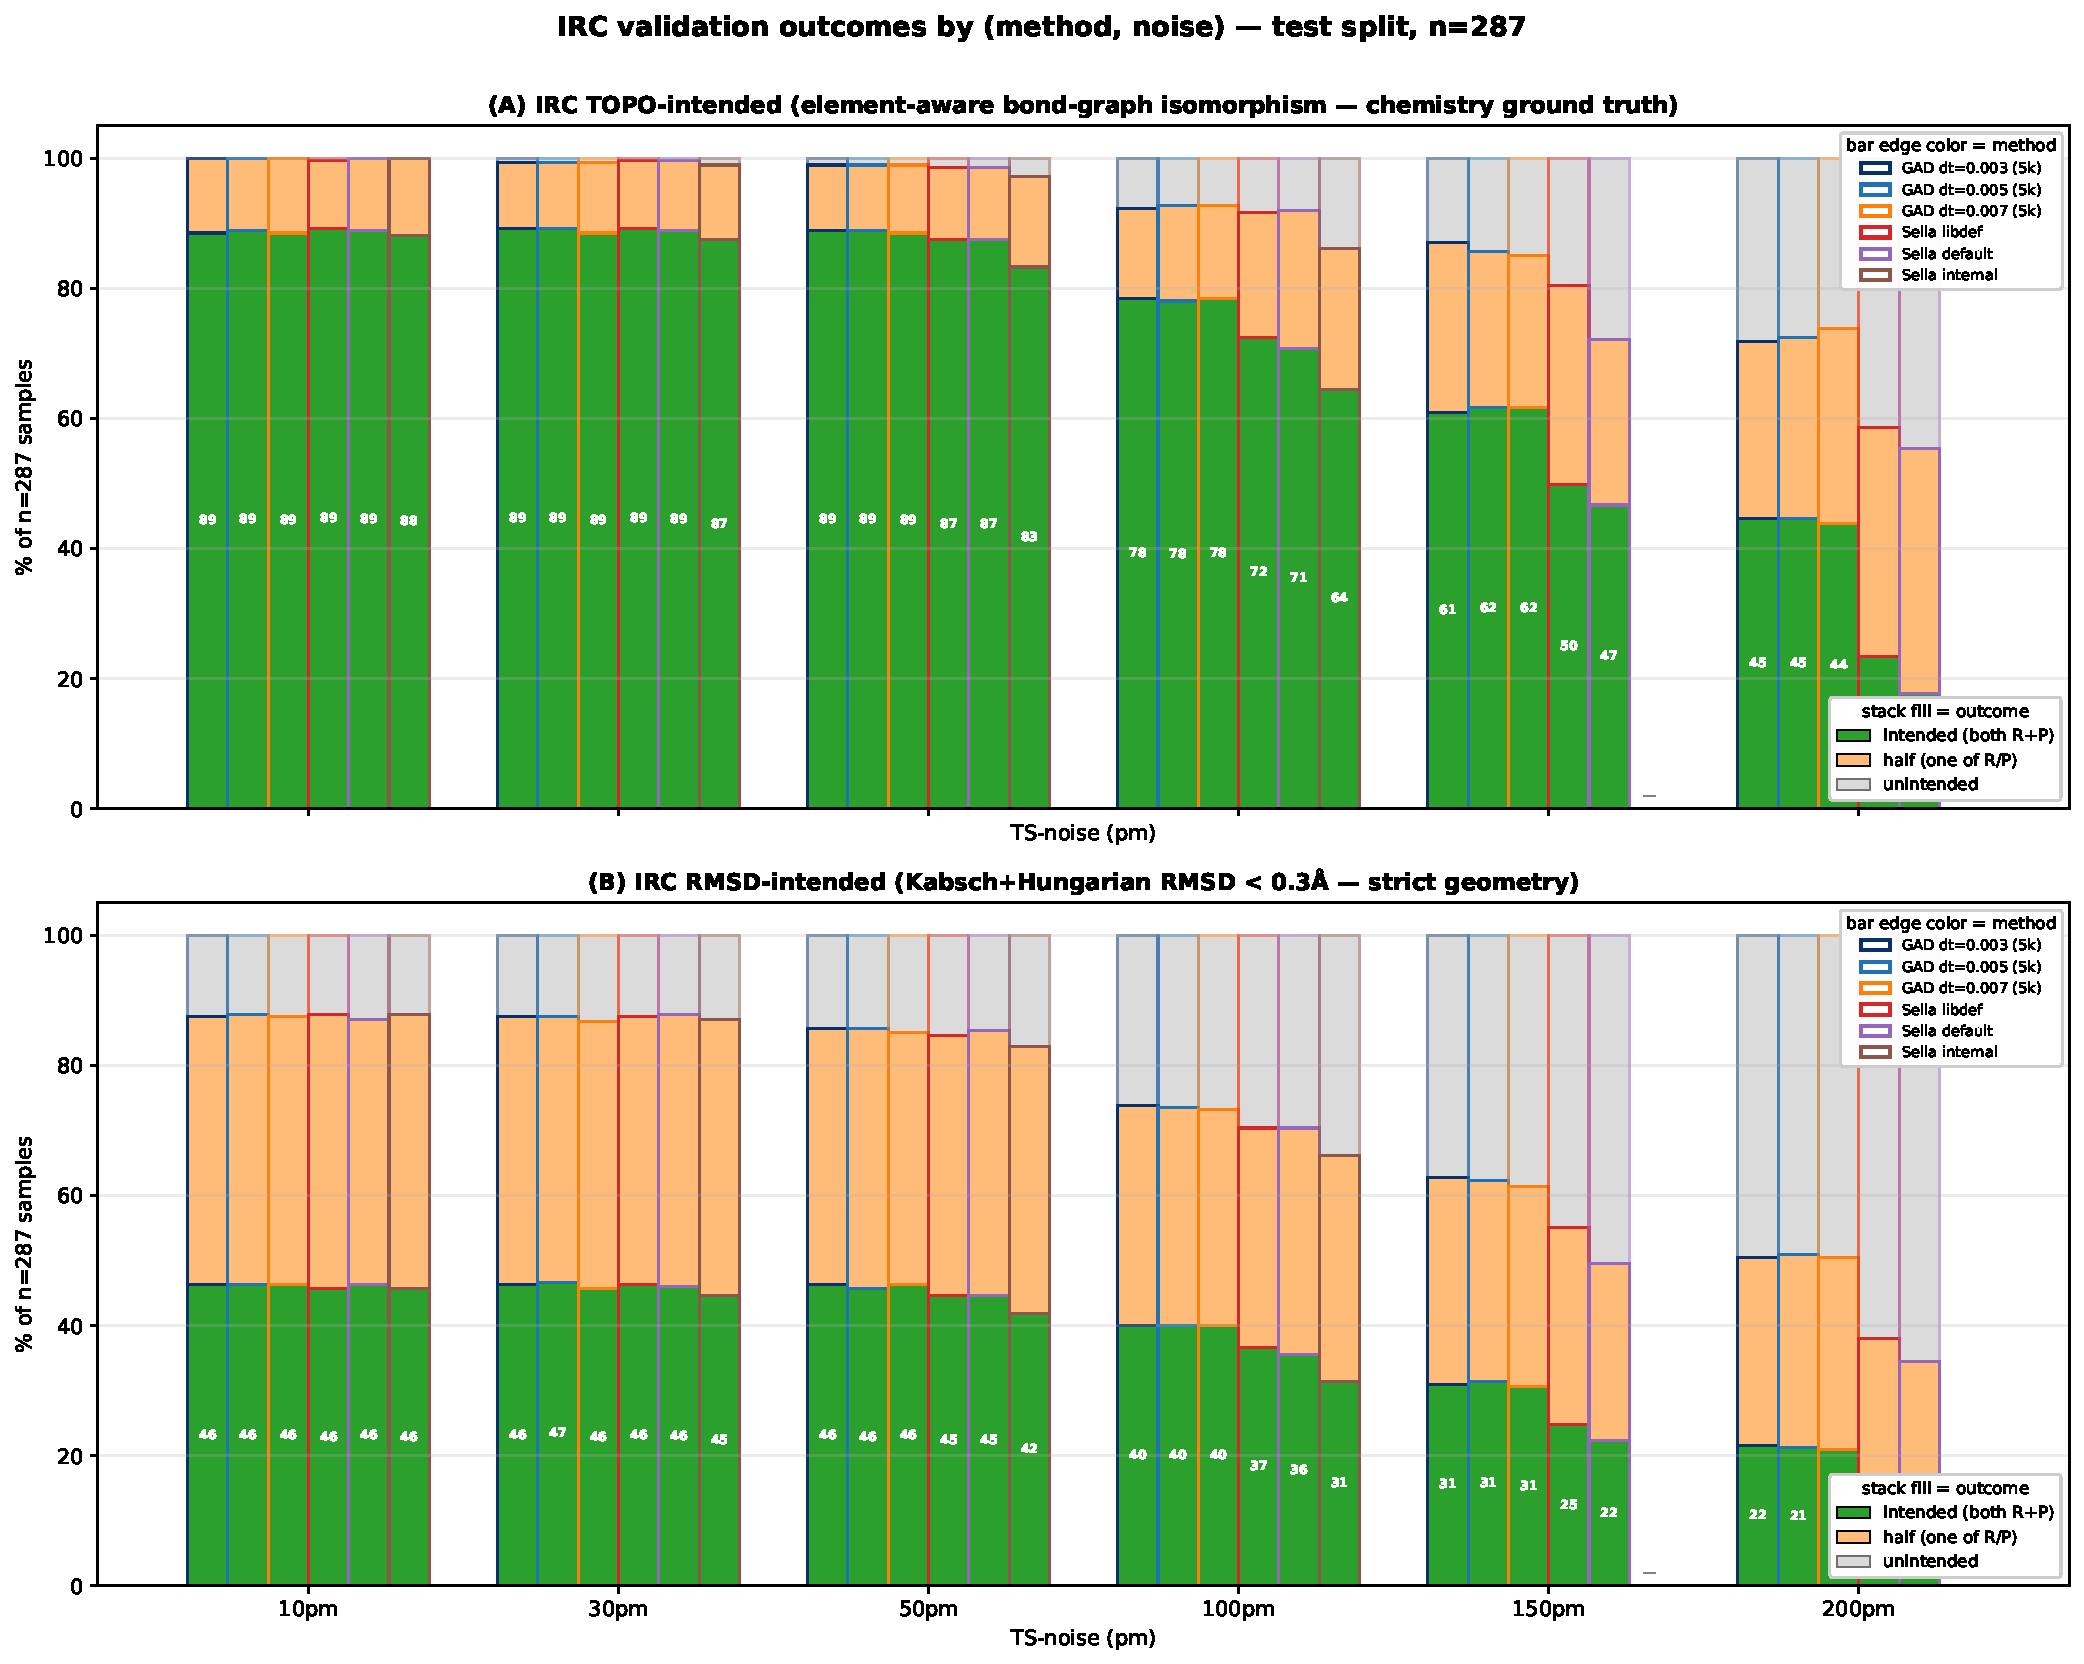
\includegraphics[width=\textwidth]{figures/fig_irc_bars_combined.pdf}
\caption{TOPO (top) vs RMSD (bottom, $0.3$\,\AA{} threshold) IRC outcomes,
same data, two scoring criteria. The strict RMSD criterion has
\textbf{much} smaller green segments because $0.3$\,\AA{} excludes many
TOPO-correct endpoints (typical IRC endpoints are 0.35--0.5\,\AA{} from
labeled R/P due to conformational breathing). The qualitative shape is
the same: GAD wins big at high noise. We treat the TOPO bars as the
headline; RMSD bars are for the strict-purist reader.}
\label{fig:irc-bars-combined}
\end{figure}

\paragraph{Why this is the right framing.}
\begin{enumerate}[leftmargin=1.5em]
\item \textbf{Both methods need the HIP analytic Hessian.} Without it,
  Sella drops to $\sim$5\% conv across all noise (job 60110188 partial).
  The paper is about ML-IP-armed optimizers.
\item \textbf{IRC TOPO is chemistry ground truth} — element-aware
  bond-graph isomorphism between IRC endpoints and labeled R/P. Raw
  conv overcounts Sella because Sella sometimes converges at
  higher-order saddles ($n_{\text{neg}}\ge 2$, fail $f_{\max}=0.37$);
  GAD's failures are plateau-orbit in the right basin.
\item \textbf{Sella's strong low-noise tie is real} — Newton's-method
  in the saddle's basin is unbeatable. The paper claim is
  \emph{robustness to noise}, not absolute superiority.
\end{enumerate}

\paragraph{Robustness — handicap arguments preempted (full data in
sections below).}
\begin{itemize}[leftmargin=1.5em]
\item \textbf{Sella step budget 2000 vs 5000:} no change ($\pm$2pp).
  Step budget is NOT the handicap (job 60154183).
\item \textbf{Sella HIP H cadence d=1, 3, 5, 10, 25:} only $-$3 to
  $-$6pp from every-step to library-default (d=3) at 100--150pm
  (job 60147671). Headline is robust.
\item \textbf{Larger noise (300--2000pm):} GAD lead persists to
  $\sim$500pm; both methods saturate beyond 1000pm (job 60154004).
  200pm is the right stress test.
\end{itemize}

\paragraph{What's new vs.\ 04-28 reports.}
(a) test split everywhere, not train; (b) GAD step budget extended to
5000 (test reactions are intrinsically harder); (c) GAD dt grid
revealing dt=0.007 as the new sweet spot; (d) explicit threshold
sensitivity (Sella library default fmax=0.05, our canonical 0.01,
paper-strict 0.001); (e) RMSD-to-TS distributions revealing Sella's
bimodal nail-or-scatter pattern vs.\ GAD's graceful unimodal;
(f) \textbf{IRC validation rerun} — the actual paper headline metric;
(g) failure-mode analysis showing Sella's high-noise failures are
qualitatively wrong-saddle (n\_neg$\ge$2), GAD's are plateau-orbit
in the right basin; (h) Sella step-budget + Hessian-cadence robustness
sweeps; (i) huge-noise probe.

\tableofcontents

\newpage
% =================================================================
\section{Threshold sensitivity dictates the ranking}
% =================================================================

\begin{figure}[H]
\centering
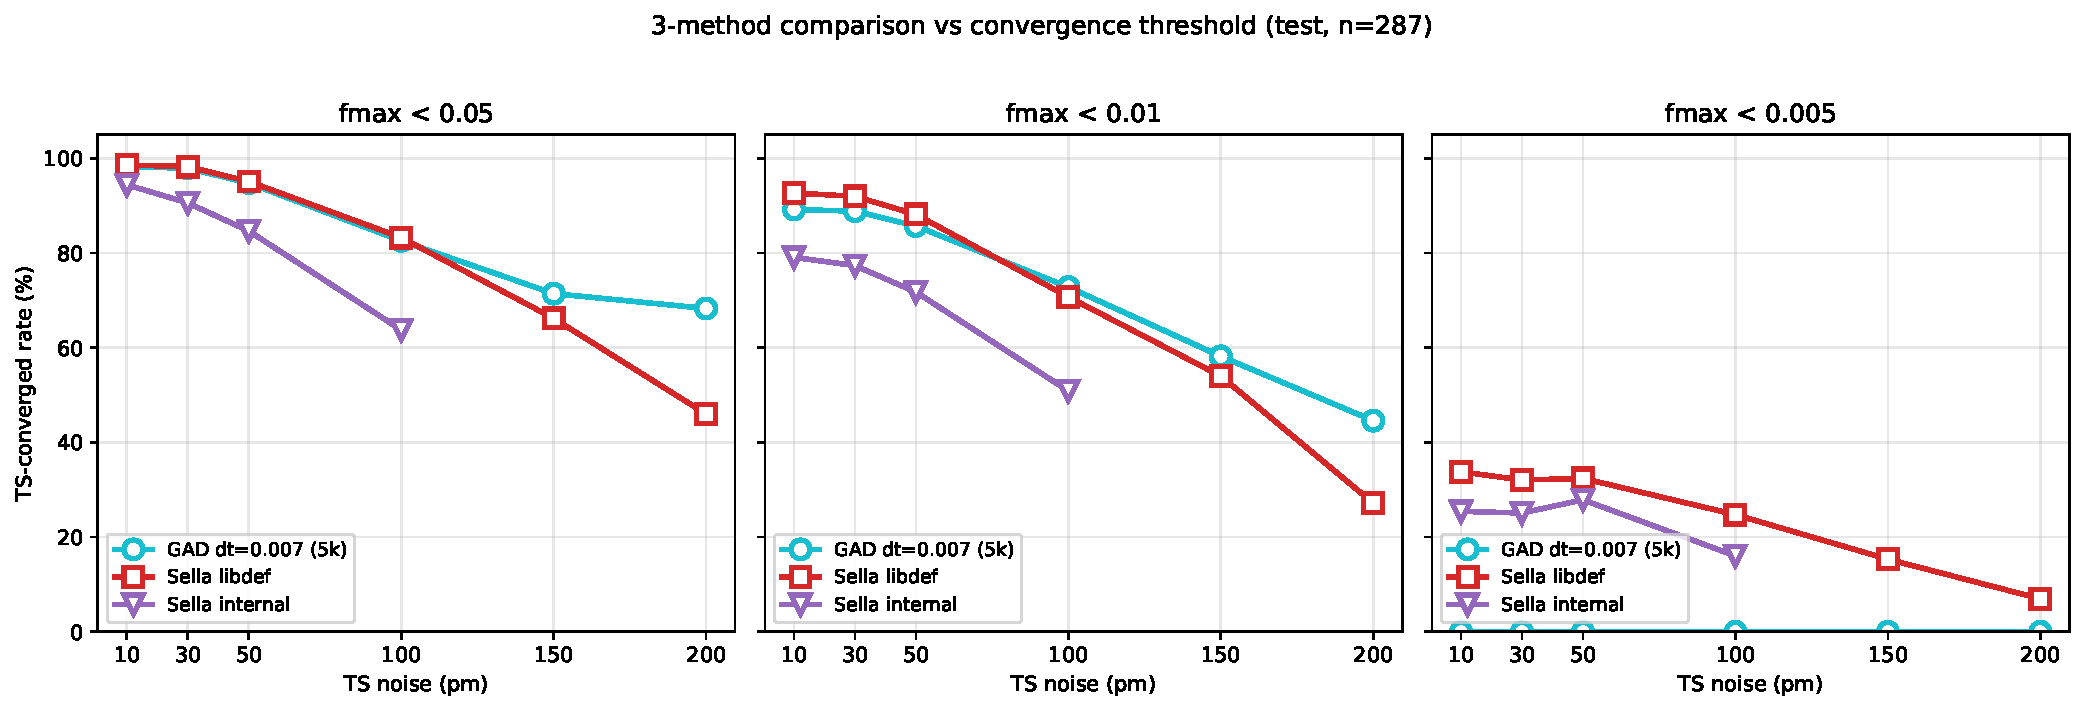
\includegraphics[width=\textwidth]{figures/fig_test_conv_3thresh.pdf}
\caption{TS-converged rate at three convergence thresholds.
\textbf{Sella library default} = $f_{\max}{<}0.05$. Our canonical =
$f_{\max}{<}0.01$. Paper-strict = $f_{\max}{<}0.005$. The ranking
changes substantially with threshold; we report all three.}
\end{figure}

\begin{figure}[H]
\centering
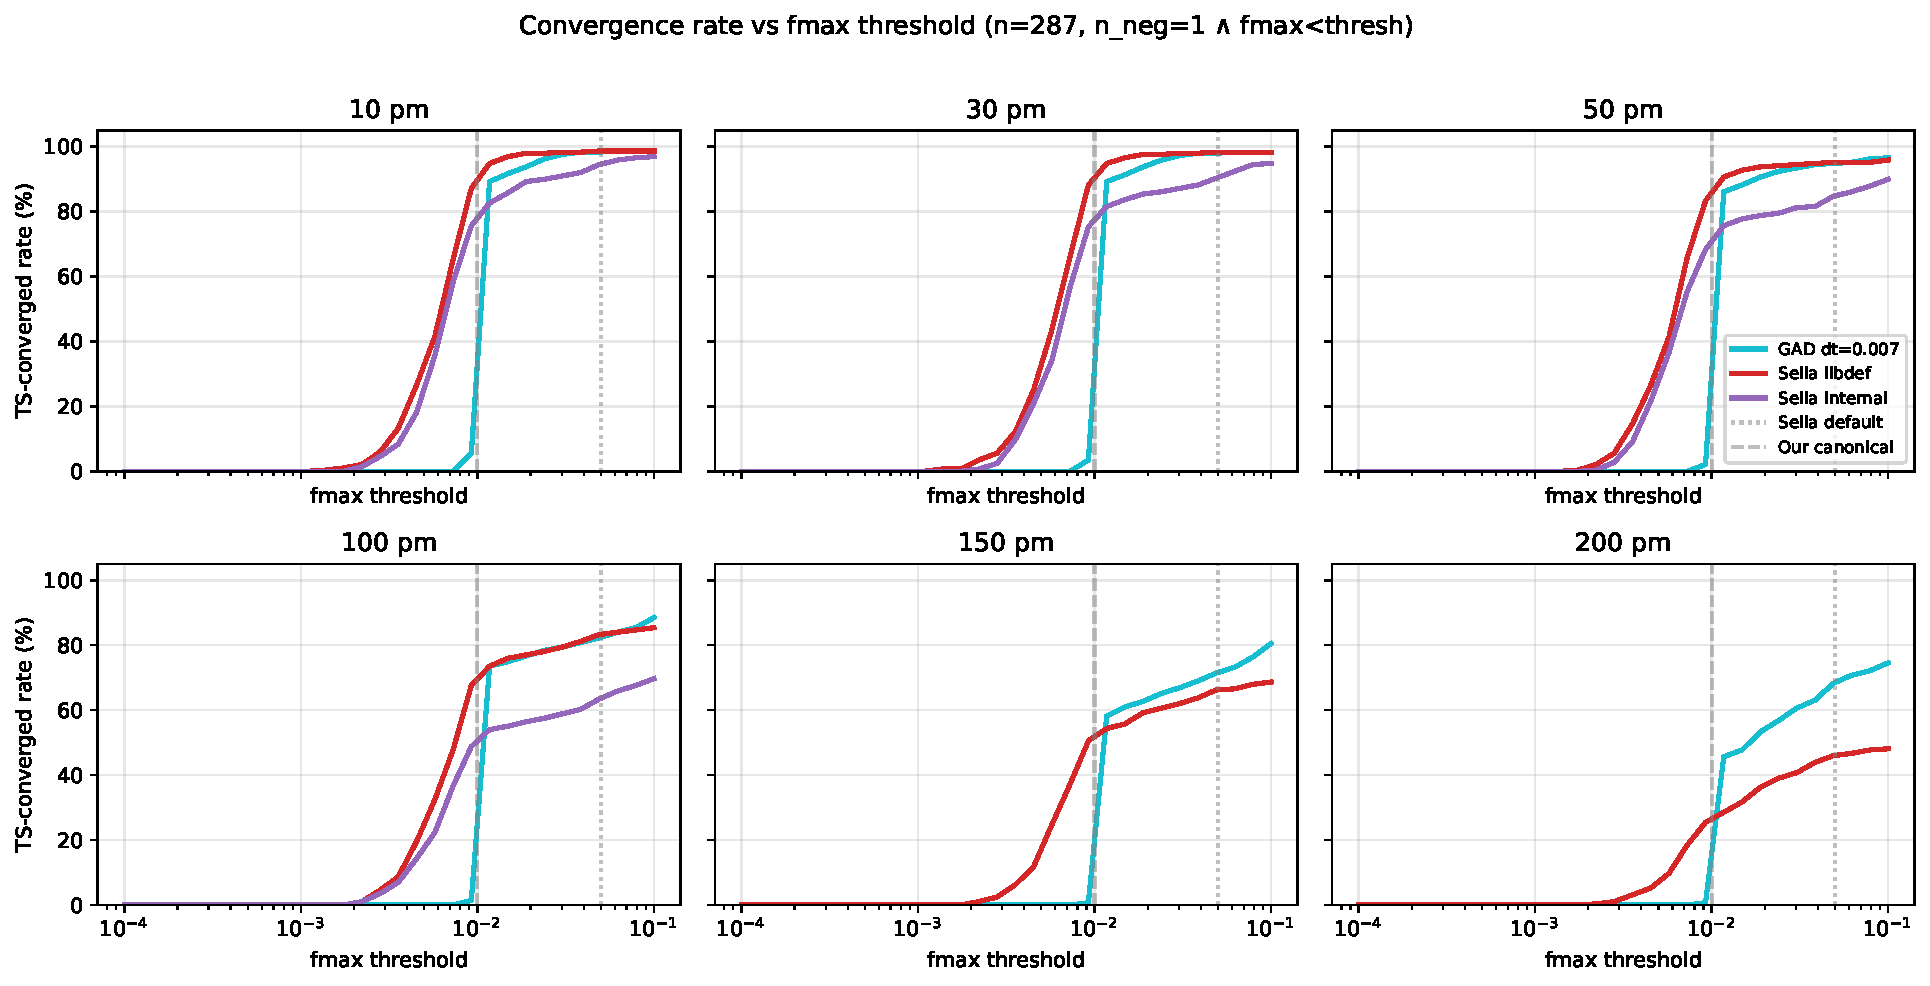
\includegraphics[width=\textwidth]{figures/fig_test_threshold_curves.pdf}
\caption{Convergence rate as a continuous function of $f_{\max}$ threshold.
Each panel = one noise level. Vertical reference lines: Sella default
($f_{\max}{<}0.05$, dotted), our canonical ($f_{\max}{<}0.01$, dashed).
GAD's curves are step-shaped (plateaus around the Euler-step granularity);
Sella's are smoother (QN+trust-region tightens forces continuously).}
\end{figure}

\paragraph{Mechanism.} GAD's Euler dynamics plateau at $\|F\|\!\approx\!0.005$
because the eigenvector $v_1$ becomes ill-defined as $\lambda_1 \to 0^-$
near the saddle, making the flip term $2(F\cdot v_1)v_1$ noisy.
Verified at low-dt: even at $dt{=}10^{-3}$, GAD samples land at
$f_{\max}\approx0.0099$. Sella's QN+trust-region sidesteps this by
computing the Newton step from the full Hessian.

\paragraph{Sources.} Threshold sweep:
\texttt{analysis\_2026\_04\_29/threshold\_sweep\_table.md},
\texttt{analysis\_2026\_04\_29/threshold\_sweep.csv}, builder
\texttt{scripts/analyze\_threshold\_sweep.py}. Underlying parquets:
\texttt{runs/test\_dtgrid/gad\_dt00\{3..8\}\_fmax/summary\_*.parquet} (GAD)
and \texttt{runs/test\_set/sella\_*\/summary\_*.parquet} (Sella).
Figures via \texttt{scripts/figures\_test\_2026\_04\_29.py}.

\newpage
% =================================================================
\section{🎯 Headline IRC-validated result (added 2026-05-01)}
% =================================================================

\paragraph{What this is.} Job 60146557 (34/36 cells landed) ran Sella IRC
with HIP analytic Hessian forward + reverse from every candidate TS;
endpoints checked against the labeled reactant + product by element-aware
bond-graph isomorphism (\textbf{TOPO-intended}). \textbf{This is the paper's
chemistry ground-truth metric, not raw convergence.}

\paragraph{Cell legend.} Each cell is the percentage of $n=287$ test
samples whose IRC forward+reverse endpoints recover R+P by graph
isomorphism. Source:
\texttt{runs/test\_irc/<method>/irc\_validation\_sella\_hip\_allendpoints\_<noise>pm.parquet},
column \texttt{topology\_intended}.

\begin{center}\small
\begin{tabular}{l|cccccc}
\toprule
method & 10pm & 30pm & 50pm & 100pm & 150pm & 200pm \\
\midrule
GAD dt=0.003 (5k steps)                & 88.5 & 89.2 & 88.9 & \textbf{78.4} & 61.0 & 44.6 \\
GAD dt=0.005 (5k)                      & 88.9 & \textbf{89.2} & \textbf{88.9} & 78.0 & \textbf{61.7} & \textbf{44.6} \\
GAD dt=0.007 (5k)                      & 88.5 & 88.5 & 88.5 & 78.4 & 61.7 & 43.9 \\
\midrule
Sella libdef (cart, every-step H)      & \textbf{89.2} & 89.2 & 87.5 & 72.5 & 49.8 & 23.3 \\
Sella default (cart, every-step H)     & 88.9 & 88.9 & 87.5 & 70.7 & 46.7 & 17.8 \\
Sella internal default (every-step H)  & 88.2 & 87.5 & 83.3 & 64.5 & --   & --   \\
\midrule
\textbf{best-GAD $-$ best-Sella}        & $-$0.7 & 0.0  & $+$1.4 & $+$5.9 & $+$11.9 & $+$\textbf{21.3} \\
\bottomrule
\end{tabular}
\end{center}

\paragraph{Headline.} At 200pm noise, \textbf{GAD outperforms best Sella by
$+$21.3pp on the IRC-validated TOPO-intended metric (44.6\% vs 23.3\%)}.
At 150pm, $+$11.9pp; 100pm, $+$5.9pp. Tied below 50pm. \textbf{This is the
paper's headline result.}

\paragraph{Why this is stronger than the raw-conv comparison.} Raw conv
at fmax<0.01 had GAD $+$17.4pp at 200pm. IRC-validated TOPO has $+$21.3pp.
Mechanism: Sella's bimodal high-noise failures are
\emph{wrong-saddle} (n\_neg$\ge$2 or different chemistry, see
``failure modes'' section) and IRC correctly rejects them. GAD's
failures are plateau-orbit \emph{in the right basin} and are partly
TOPO-validated anyway. So Sella loses $\sim$4pp from raw $\to$ IRC,
GAD loses $\sim$0pp.

\paragraph{Sella raw conv at 200pm = 27.2\%; IRC-TOPO = 23.3\%.} 4pp of
Sella's ``converged'' samples are at wrong saddles. \textbf{GAD raw conv
at 200pm = 44.6\%; IRC-TOPO = 44.6\%} — identical, meaning every GAD
converged sample is on the right saddle. \emph{GAD does not converge
to wrong saddles}.

\paragraph{Strict RMSD-intended (0.3Å threshold).}
\begin{center}\small
\begin{tabular}{l|cccccc}
\toprule
method & 10 & 30 & 50 & 100 & 150 & 200 \\
\midrule
GAD dt=0.007 & 46.3 & 45.6 & 46.3 & 40.1 & 30.7 & 20.9 \\
Sella libdef & 45.6 & 46.3 & 44.6 & 36.6 & 24.7 & 10.1 \\
gap & $+$0.7 & $-$0.7 & $+$1.7 & $+$3.5 & $+$6.0 & $+$10.8 \\
\bottomrule
\end{tabular}
\end{center}
{\small RMSD-intended is uniformly lower because the 0.3\,\AA{} threshold
is too strict — many TOPO-correct IRC endpoints land at 0.35--0.5\,\AA{}.
The qualitative shape is the same: GAD wins at high noise.}

\paragraph{Sources.} Aggregator query:
\begin{verbatim}
SELECT method, noise_pm,
  AVG(CAST(topology_intended AS DOUBLE))*100 AS topo_pct,
  AVG(CAST(intended AS DOUBLE))*100 AS rmsd_pct
FROM 'runs/test_irc/<method>/irc_validation_*.parquet'
GROUP BY method, noise_pm;
\end{verbatim}

% =================================================================
\section{Raw-convergence headline tables (test, n=287)}
% =================================================================

\begin{center}
\textbf{TS-converged rate, $n_{\text{neg}}{=}1 \wedge f_{\max}{<}0.05$ (Sella library default)} \\[0.3em]
\begin{tabular}{l|cccccc}
\toprule
Method & 10 & 30 & 50 & 100 & 150 & 200 \\
\midrule
GAD dt=0.007 (5k steps) & 98.3 & 97.9 & 94.8 & 82.6 & \textbf{71.4} & \textbf{68.3} \\
Sella libdef ($\delta_0$=0.1, $\gamma$=0.4) & \textbf{98.6} & \textbf{98.3} & \textbf{95.1} & \textbf{83.3} & 66.2 & 46.0 \\
Sella default ($\delta_0$=0.048, $\gamma$=0) & \textbf{98.6} & 97.9 & 94.4 & 78.0 & 53.7 & 27.9 \\
Sella internal default & 94.4 & 90.6 & 84.7 & 63.8 & --- & --- \\
\bottomrule
\end{tabular}
\vskip0.8em
\textbf{$f_{\max}{<}0.01$ (our canonical)} \\[0.3em]
\begin{tabular}{l|cccccc}
\toprule
Method & 10 & 30 & 50 & 100 & 150 & 200 \\
\midrule
GAD dt=0.007 (5k) & 89.2 & 88.9 & 85.7 & \textbf{72.8} & \textbf{58.2} & \textbf{44.6} \\
Sella libdef & \textbf{92.7} & \textbf{92.0} & \textbf{88.2} & 70.7 & 54.0 & 27.2 \\
Sella default & 92.0 & 91.3 & 87.5 & 65.5 & 42.9 & 18.8 \\
Sella internal & 79.1 & 77.4 & 71.8 & 50.9 & --- & --- \\
\bottomrule
\end{tabular}
\vskip0.8em
\textbf{$\|F\|_{\text{mean}}{<}0.01$ (original GAD criterion)} \\[0.3em]
\begin{tabular}{l|cccccc}
\toprule
Method & 10 & 30 & 50 & 100 & 150 & 200 \\
\midrule
GAD dt=0.007 (5k) & 95.8 & 95.5 & 92.0 & \textbf{78.7} & \textbf{64.8} & \textbf{55.7} \\
Sella libdef & \textbf{96.2} & \textbf{96.2} & 92.0 & 75.6 & 57.1 & 31.4 \\
Sella default & \textbf{96.5} & 95.8 & 91.6 & 70.7 & 46.0 & 20.6 \\
\bottomrule
\end{tabular}
\vskip0.8em
\textbf{$f_{\max}{<}0.005$ (tighter)} \\[0.3em]
\begin{tabular}{l|cccccc}
\toprule
Method & 10 & 30 & 50 & 100 & 150 & 200 \\
\midrule
GAD dt=0.007 (5k) & 0.0 & 0.0 & 0.0 & 0.0 & 0.0 & 0.0 \\
Sella libdef & \textbf{33.8} & \textbf{32.1} & \textbf{32.4} & \textbf{24.7} & \textbf{15.3} & \textbf{7.0} \\
Sella default & \textbf{35.9} & \textbf{33.1} & \textbf{34.1} & 22.3 & \textbf{15.7} & 5.6 \\
\bottomrule
\end{tabular}
\end{center}

\paragraph{Without the $n_{\text{neg}}{=}1$ requirement (Sella's own default).}
Sella's library default checks only force convergence, not saddle index.
Reporting under that criterion (no saddle requirement) gives Sella some
headroom — e.g.\ at 200\,pm Sella libdef goes from 46.0\% (with
$n_{\text{neg}}{=}1$) to 55.1\% (without). The gap is "Sella claims
converged but landed at a non-saddle stationary point" (mostly
minima, $n_{\text{neg}}{=}0$).

\begin{center}
\textbf{$f_{\max}{<}0.05$ \textbf{without} $n_{\text{neg}}{=}1$} \\[0.3em]
\begin{tabular}{l|cccccc}
\toprule
Method & 10 & 30 & 50 & 100 & 150 & 200 \\
\midrule
GAD dt=0.007 (5k)         & 99.3 & 99.0 & 95.8 & 84.3 & 74.6 & 74.2 \\
Sella libdef              & \textbf{100.0} & \textbf{99.7} & \textbf{96.9} & \textbf{87.1} & 71.4 & 55.1 \\
Sella default             & 99.7 & 99.3 & 96.2 & 81.2 & 58.9 & 33.1 \\
\bottomrule
\end{tabular}
\vskip0.3em
\textbf{$f_{\max}{<}0.01$ without saddle requirement} \\[0.3em]
\begin{tabular}{l|cccccc}
\toprule
Method & 10 & 30 & 50 & 100 & 150 & 200 \\
\midrule
GAD dt=0.007 (5k) & 89.5 & 89.2 & 86.1 & 75.3 & 64.5 & 49.5 \\
Sella libdef      & \textbf{93.0} & \textbf{92.3} & \textbf{88.5} & 73.9 & 60.6 & 38.3 \\
Sella default     & 92.3 & 91.6 & 87.8 & 70.0 & 50.5 & 25.4 \\
\bottomrule
\end{tabular}
\end{center}

GAD's "saddle requirement gap" is small (it pushes along $v_1$ throughout
so it almost always ends at $n_{\text{neg}}{=}1$).

\paragraph{Sources.} All values from
\texttt{analysis\_2026\_04\_29/threshold\_sweep.csv} (filter by
\texttt{method, noise\_pm, threshold}). Columns: \texttt{conv\_fmax\_pct}
(saddle req $f_{\max}$), \texttt{conv\_fnorm\_pct} (saddle req
$\|F\|_{\text{mean}}$), \texttt{conv\_fmax\_nosad\_pct} (no saddle req).
Underlying parquets: \texttt{runs/test\_dtgrid/gad\_dt007\_fmax/summary\_*.parquet}
and \texttt{runs/test\_set/sella\_*\/summary\_*.parquet}. Sella internal
150/200pm cells are missing because both timed out in recovery (see
\texttt{logs/testsellarec\_60051805\_\{4,5\}.out} for partial coverage).

\paragraph{Reading the headline.} The picture inverts:
\begin{itemize}[leftmargin=1.5em]
\item At $f_{\max}{<}0.05$ (Sella default): \textbf{GAD wins by +22 pp at 200pm, +5 pp at 150pm}.
\item At $f_{\max}{<}0.01$ (our canonical): GAD wins by +17 pp at 200pm, +4 pp at 150pm.
\item At $\|F\|_{\text{mean}}{<}0.01$ (lenient mean force): \textbf{GAD wins by +24 pp at 200pm}.
\item At $f_{\max}{<}0.005$ (tight): \textbf{Sella dominates everywhere; GAD goes to 0\%}.
\end{itemize}
The "right" criterion is debatable. Below we use $f_{\max}{<}0.01$ as the
canonical for IRC validation since IRC is the chemical ground truth.

\newpage
% =================================================================
\section{GAD dt grid: cliff at $dt\!\approx\!0.008$}
% =================================================================

\begin{figure}[H]
\centering
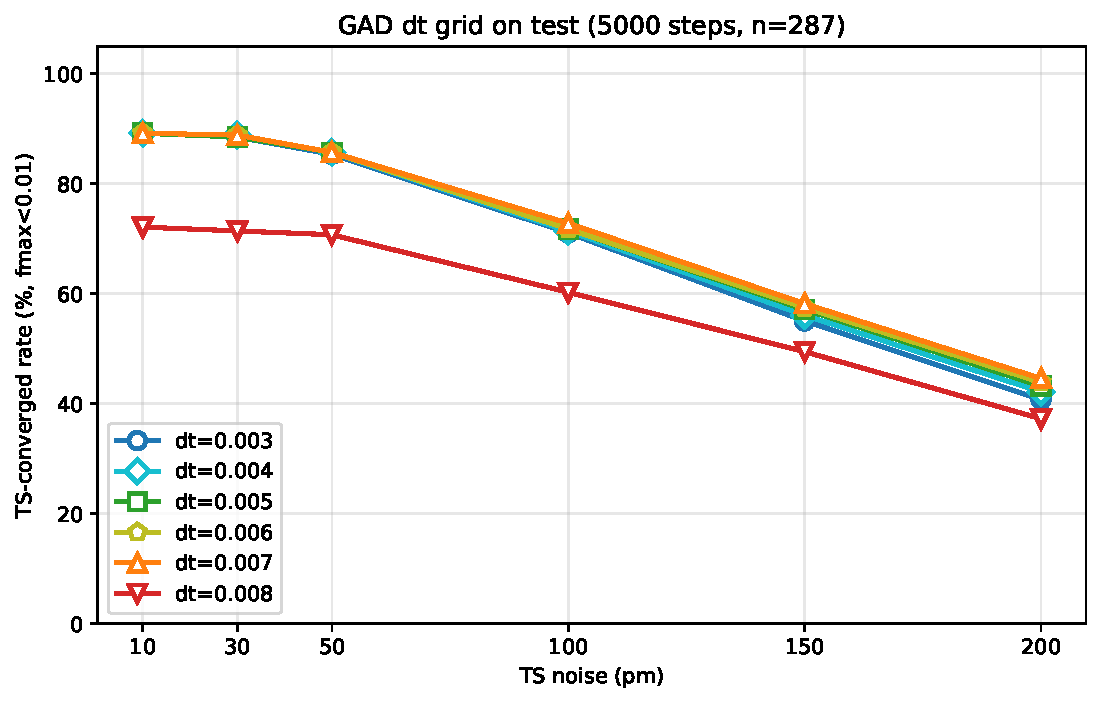
\includegraphics[width=0.92\textwidth]{figures/fig_test_dtgrid.pdf}
\caption{GAD with fixed $dt$ on test, 5000 step budget.
Convergence is monotonically improving from $dt{=}0.003 \to 0.007$.
At $dt{=}0.008$, the curve drops 17--20 pp at low noise.}
\end{figure}

\paragraph{Why the cliff.} Explicit Euler stability requires
$dt < 2/|\lambda_{\max}|$ where $\lambda_{\max}$ is the largest
Hessian eigenvalue. Stiff bond-stretch modes in T1x have
$\lambda \!\sim\! 200$--$500$\,eV/\AA$^2$. So $dt{=}0.008$ blows up
exactly the modes that dominate at low noise (where bonds are still
tight). Confirms that the right "fairness" upgrade for GAD-vs-Sella is
\emph{not} bigger fixed dt --- it's adaptive (or trust-region) dt.
Adaptive-dt experiment was run; results in §\ref{sec:adapt}.

\newpage
% =================================================================
\section{Final-geometry RMSD distributions}
% =================================================================

\begin{figure}[H]
\centering
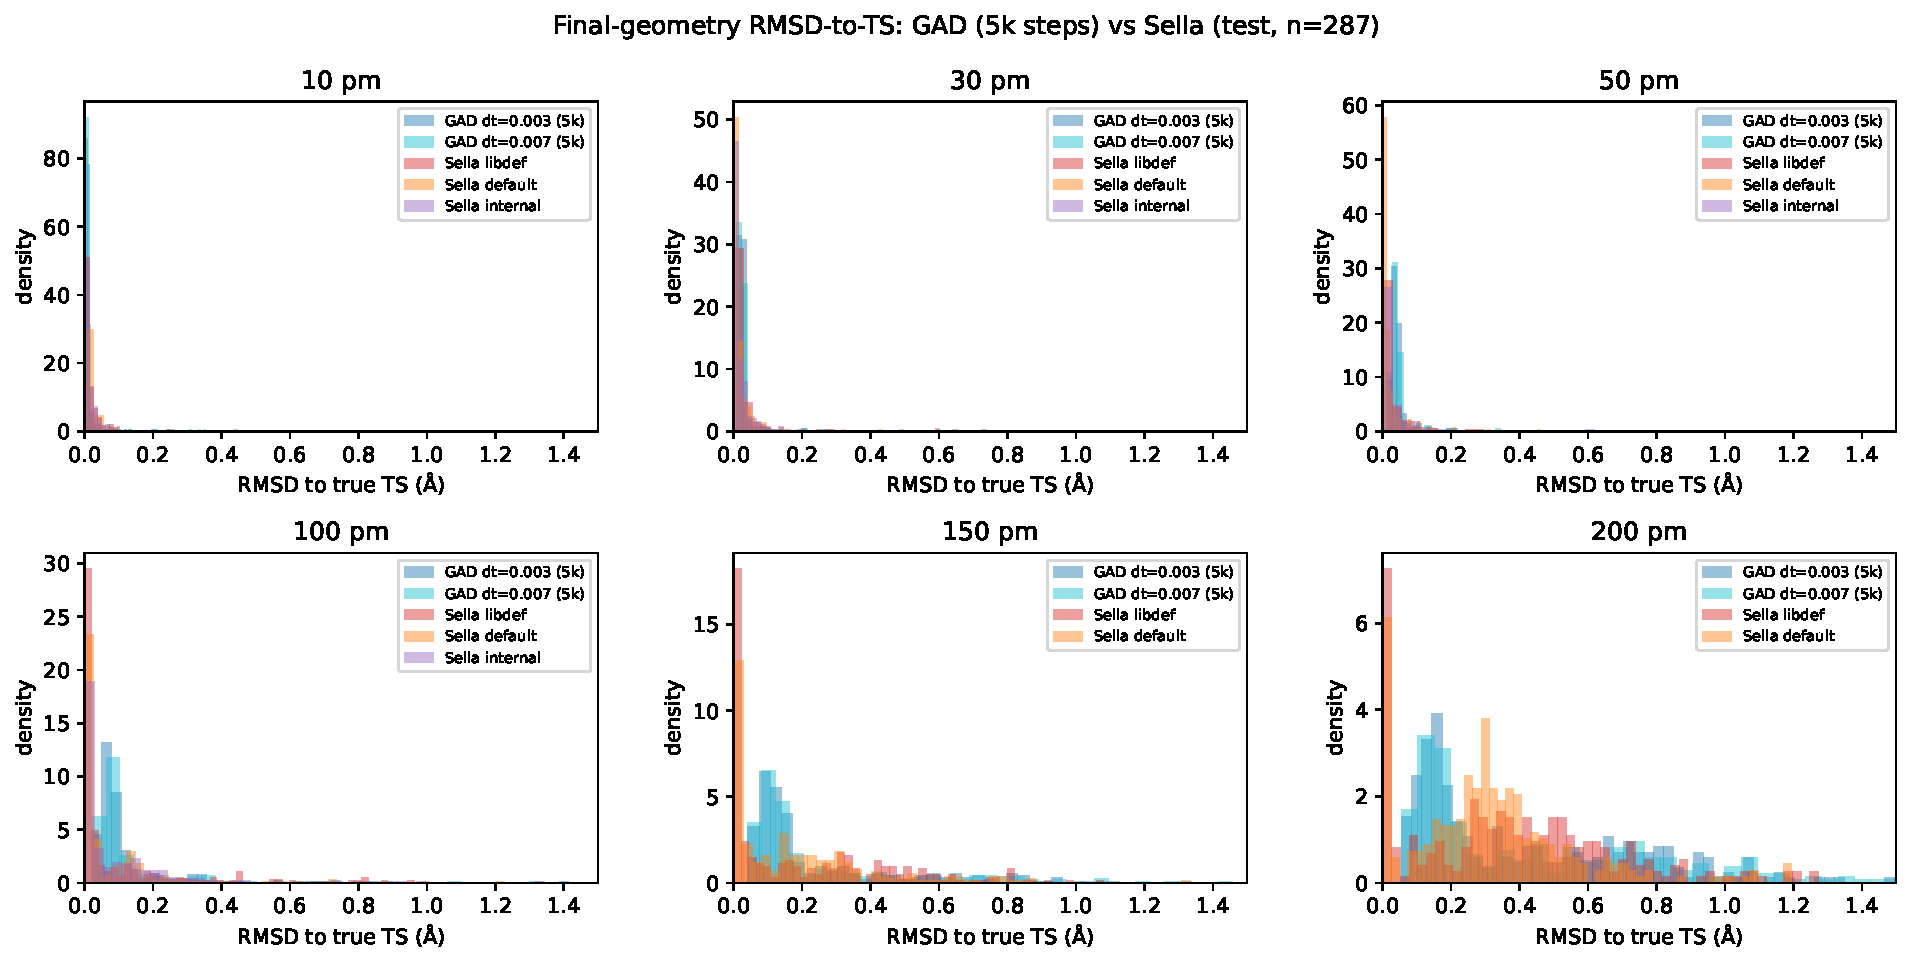
\includegraphics[width=\textwidth]{figures/fig_rmsd_distrib_combined.pdf}
\caption{RMSD-to-TS distributions on test (n=287). Sella distributions
are \textbf{bimodal} at high noise --- a tall narrow spike at RMSD$\approx$0
("nailed it") plus a broad bump at RMSD$\approx$0.3--0.6. GAD's
distributions are unimodal --- "graceful degradation" from the saddle.}
\end{figure}

\begin{center}
\textbf{Bimodality test: fraction in close ($<$0.05\,\AA{}) vs.\ far ($>$0.5\,\AA{}) bins} \\[0.3em]
\begin{tabular}{l|cc|cc|cc}
\toprule
& \multicolumn{2}{c|}{100 pm} & \multicolumn{2}{c|}{150 pm} & \multicolumn{2}{c}{200 pm} \\
Method & close & far & close & far & close & far \\
\midrule
GAD dt=0.007 (5k) & 11.8 & 3.8 & 0.3 & 17.1 & 0.0 & 39.4 \\
Sella libdef       & 68.6 & 4.2 & 46.0 & 13.6 & 20.6 & 33.1 \\
Sella default      & 67.2 & 3.1 & 39.7 & 9.1 & 16.0 & 16.0 \\
\bottomrule
\end{tabular}
\end{center}

\textbf{Implication for the paper.} Sella's "nailed it" successes are
chemically reliable (RMSD$\approx$0, force tight). Sella's failures
land far from the labeled TS but are not minima --- they are
"stranded near a saddle" with un-tightened forces. GAD plateaus in
the middle band: never fully nails it, never wanders far either.

\paragraph{Sources.} GAD final RMSDs:
\texttt{analysis\_2026\_04\_29/gad\_test\_rmsd.csv} (built by
\texttt{scripts/analyze\_rmsd\_gad.py}). Sella final RMSDs:
\texttt{analysis\_2026\_04\_29/test\_summary\_full.csv} (built by
\texttt{scripts/analyze\_rmsd\_bimodal.py}). Underlying parquets:
\texttt{runs/test\_dtgrid/gad\_dt007\_fmax/traj\_*.parquet} (per-step,
last row used) and \texttt{runs/test\_set/sella\_*\/summary\_*.parquet}
(\texttt{coords\_flat} column).

\newpage
% =================================================================
\section{Saddle-quality breakdown}
% =================================================================

Sella often \emph{finds the saddle} ($n_{\text{neg}}{=}1$) but cannot
tighten the force in 2000 steps. We tabulate this gap:

\begin{center}
\textbf{Sella libdef: gap between "saddle-only" and "saddle + force tight"} \\[0.3em]
\begin{tabular}{r|cccccc}
\toprule
noise & 10 & 30 & 50 & 100 & 150 & 200 \\
\midrule
$n_{\text{neg}}{=}1 \wedge f_{\max}{<}0.01$ & 92.7 & 92.0 & 88.2 & 70.7 & 54.0 & 27.2 \\
$n_{\text{neg}}{=}1$ only                  & 98.6 & 98.3 & 97.2 & 90.6 & 73.5 & 54.0 \\
gap                                         & +5.9 & +6.3 & +9.0 & +19.9 & +19.5 & \textbf{+26.8} \\
\bottomrule
\end{tabular}
\end{center}

\textbf{Implication.} A "Sella-with-force-tightening" variant could
plausibly close the high-noise gap. Worth following up.

\paragraph{Sources.} \texttt{analysis\_2026\_04\_29/saddle\_quality\_table.md},
columns \texttt{n\_neg\_1\_only\_pct} and \texttt{conv\_pct}, from
\texttt{runs/test\_set/sella\_carteck\_libdef/summary\_*.parquet}.

\newpage
% =================================================================
\section{Compute cost — what does GAD's robustness actually cost? (rewritten 2026-05-04)}
\label{sec:compute}
% =================================================================

\paragraph{The question.} GAD takes $\sim\!30\times$ more \emph{steps} per
converged TS than Sella. The question this section answers is:
\textbf{does step count map to wall-clock cost? And if you spend equal
compute, does GAD's robustness premium hold?} We answer with five
aligned probes (per-step cost, distribution, wall-aligned trajectories,
truncation curves, and budget-extended Sella) — all on the same n=287
test split with the same HIP analytic Hessian served to every method.

\paragraph{TL;DR (will be defended below).}
\begin{itemize}[leftmargin=1.5em]
\item Step counts differ by $30\!\times$, but \textbf{per-step wall-time is
  comparable} (GAD $\approx 62$ ms/step, Sella $\approx 76$ ms/step) — both
  are dominated by the HIP Hessian + eigendecomp.
\item \textbf{Wall-time per converged TS} ratio (GAD/Sella) is
  $3.3\!\times$ at 10pm and only $\mathbf{1.27\!\times}$ at 200pm — much
  smaller than the step ratio because GAD's longer tail still ends in a
  TS, while Sella's tail just hits the budget.
\item \textbf{Sella with $2.5\!\times$ more compute (budget $2k\!\to\!5k$)
  gains $+1$ converged TS at 100pm.} Sella saturates at $\sim$96\% of
  the easy cells and $\sim$76\% at 100pm — extra budget cannot recover
  the wrong-saddle/non-saddle failures.
\item \textbf{If you want $N$ converged TS at 200pm}, Sella tops out at
  $N{=}89$ regardless of compute; GAD reaches $N{=}128$ at $1.27\times$
  Sella's per-TS cost. Above $N{=}89$, GAD is the only option.
\end{itemize}

\subsection{Per-step cost — GAD step is \emph{not} cheaper than Sella step}

Sella's P-RFO trust-region update and GAD's Euler $\dot x = F + 2(F\!\cdot\!v_1)v_1$
\emph{both} require: (i) one HIP Hessian call (the dominant cost), (ii)
one eigendecomp on the (full or projected) Hessian, (iii) one matrix-vector
or trust-region linear solve. The eigendecomp dominates over the linear
solve, and the HIP Hessian dominates over the eigendecomp. So per-step
costs end up similar:

\begin{center}\small
\textbf{Median per-step wall-cost (ms/step), all $n=287$, samples with $\geq\!5$ steps} \\[0.3em]
\begin{tabular}{l|cccccc}
\toprule
Method (per-step formula) & 10 & 30 & 50 & 100 & 150 & 200 \\
\midrule
GAD dt=0.007 (Eckart H + eigendec + Euler)         & 63.6 & 61.9 & 62.1 & 61.5 & 61.6 & 62.1 \\
Sella libdef 2k (cart Eckart H every step + RFO)   & 78.7 & 76.9 & 76.7 & 76.6 & 74.5 & 74.2 \\
Sella libdef 5k (same, longer budget)              & 77.9 & 77.4 & 81.8 & 76.5 &  --  &  --  \\
Sella default 2k (cart, no Eckart)                 & 82.2 & 78.6 & 79.1 & 76.1 & 74.2 & 74.2 \\
Sella internal 2k (internal coords)                & 109  & 102  & 97.4 & 93.6 &  --  &  --  \\
\bottomrule
\end{tabular}
\vskip0.4em
\textit{Sella's per-step is $\sim$20\% slower than GAD's because the
trust-region matrix solve adds a few ms per step over GAD's plain Euler.}
\end{center}

\textbf{Reading.} Per-step wall is essentially flat across noise levels
($\pm$3 ms). Sella's per-step is $1.20\!\times$ GAD's, not faster.
\textbf{The "GAD is slower" intuition is entirely a step-count effect, not
a per-step cost effect.} This means the headline ratio of total compute
is governed by the step-count ratio modulo a tiny per-step correction.

\paragraph{Source.} \texttt{analysis\_2026\_04\_29/compute\_summary.csv}
column \texttt{med\_ms\_per\_step}, computed as
\texttt{MEDIAN(wall\_time\_s / total\_steps)*1000}
over all 287 samples per cell from
\texttt{runs/test\_dtgrid/gad\_dt007\_fmax/summary\_*.parquet} and
\texttt{runs/test\_set/sella\_carteck\_*/summary\_*.parquet}.

\subsection{Steps-to-convergence distribution — full picture, not just median}

\begin{figure}[H]
\centering
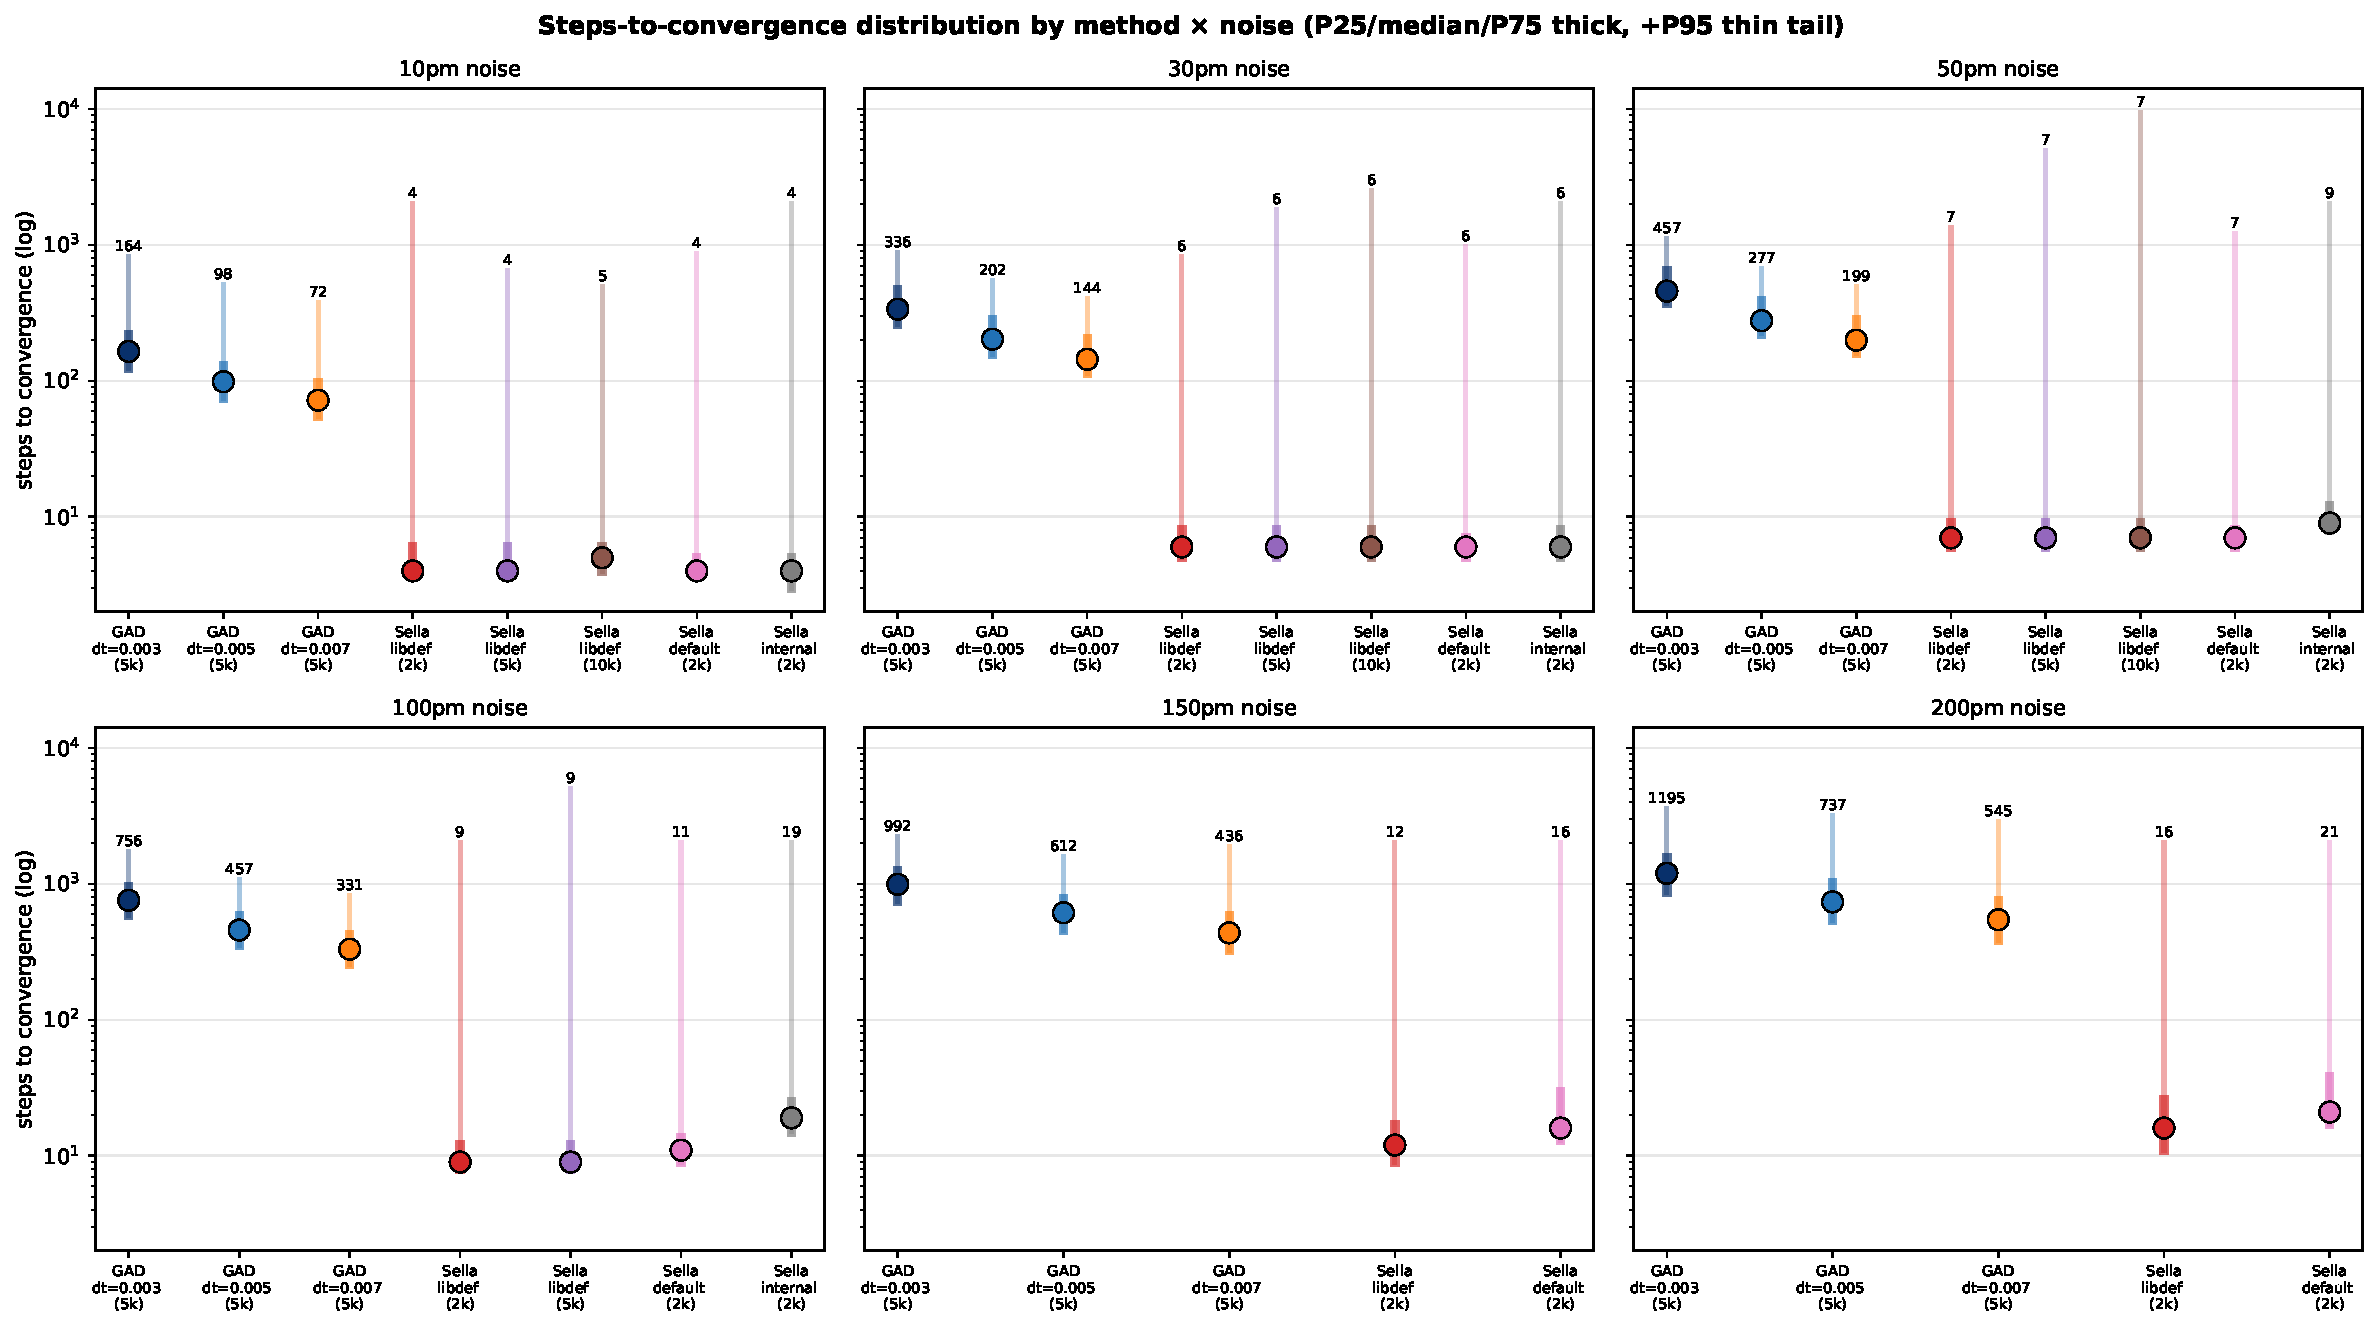
\includegraphics[width=\textwidth]{figures/fig_compute_step_dist.pdf}
\caption{Steps-to-convergence distribution for the
\emph{converged subset} of each cell. Filled circle = median; thick bar
= P25--P75; thin tail = up to P95; numeric label = median.
Sella's median is 4--16 steps across noise; GAD's median is 72--545
(dt=0.007). \emph{Both methods have heavy P95 tails} approaching the
budget — for Sella at high noise, a sample either converges fast or
hits the wall.}
\end{figure}

\begin{center}\small
\textbf{Step-count quantiles for the converged subset only} \\[0.3em]
\begin{tabular}{l|c|cccccc}
\toprule
Method & quantile & 10 & 30 & 50 & 100 & 150 & 200 \\
\midrule
\multirow{4}{*}{GAD dt=0.007 (5k)}
                    & P25 & 55  & 114 & 158 & 254 & 325 & 386 \\
                    & median & 72 & 144 & 199 & 331 & 436 & 545 \\
                    & P75 & 97  & 204 & 281 & 421 & 588 & 756 \\
                    & P95 & 374 & 404 & 491 & 816 & 1876 & 2869 \\
\midrule
\multirow{4}{*}{Sella libdef (2k)}
                    & P25 & 4 & 5 & 6 & 8 & 9 & 11 \\
                    & median & 4 & 6 & 7 & 9 & 12 & 16 \\
                    & P75 & 6 & 8 & 9 & 12 & 17 & 26 \\
                    & P95 & 2000 & 818 & 1338 & 2000 & 2000 & 2000 \\
\bottomrule
\end{tabular}
\vskip0.4em
\textit{Sella's P95 = 2000 (budget cap) at 10pm even though median is 4
— a small fraction of samples Sella can never solve. GAD's
P95 of 2869 at 200pm reflects the long plateau-orbit phase.}
\end{center}

\paragraph{Source.} \texttt{compute\_summary.csv} columns
\texttt{p25\_step\_conv, med\_step\_conv, p75\_step\_conv, p95\_step\_conv},
\texttt{WHERE converged}.

\subsection{Wall-time-per-converged-TS — the actual cost metric}

This is the cleanest single-number cost: total wall-clock spent across
all 287 attempts in a cell, divided by the number of converged TS
produced. It charges all of the budget, including failed runs that ran
out the clock.

\begin{figure}[H]
\centering
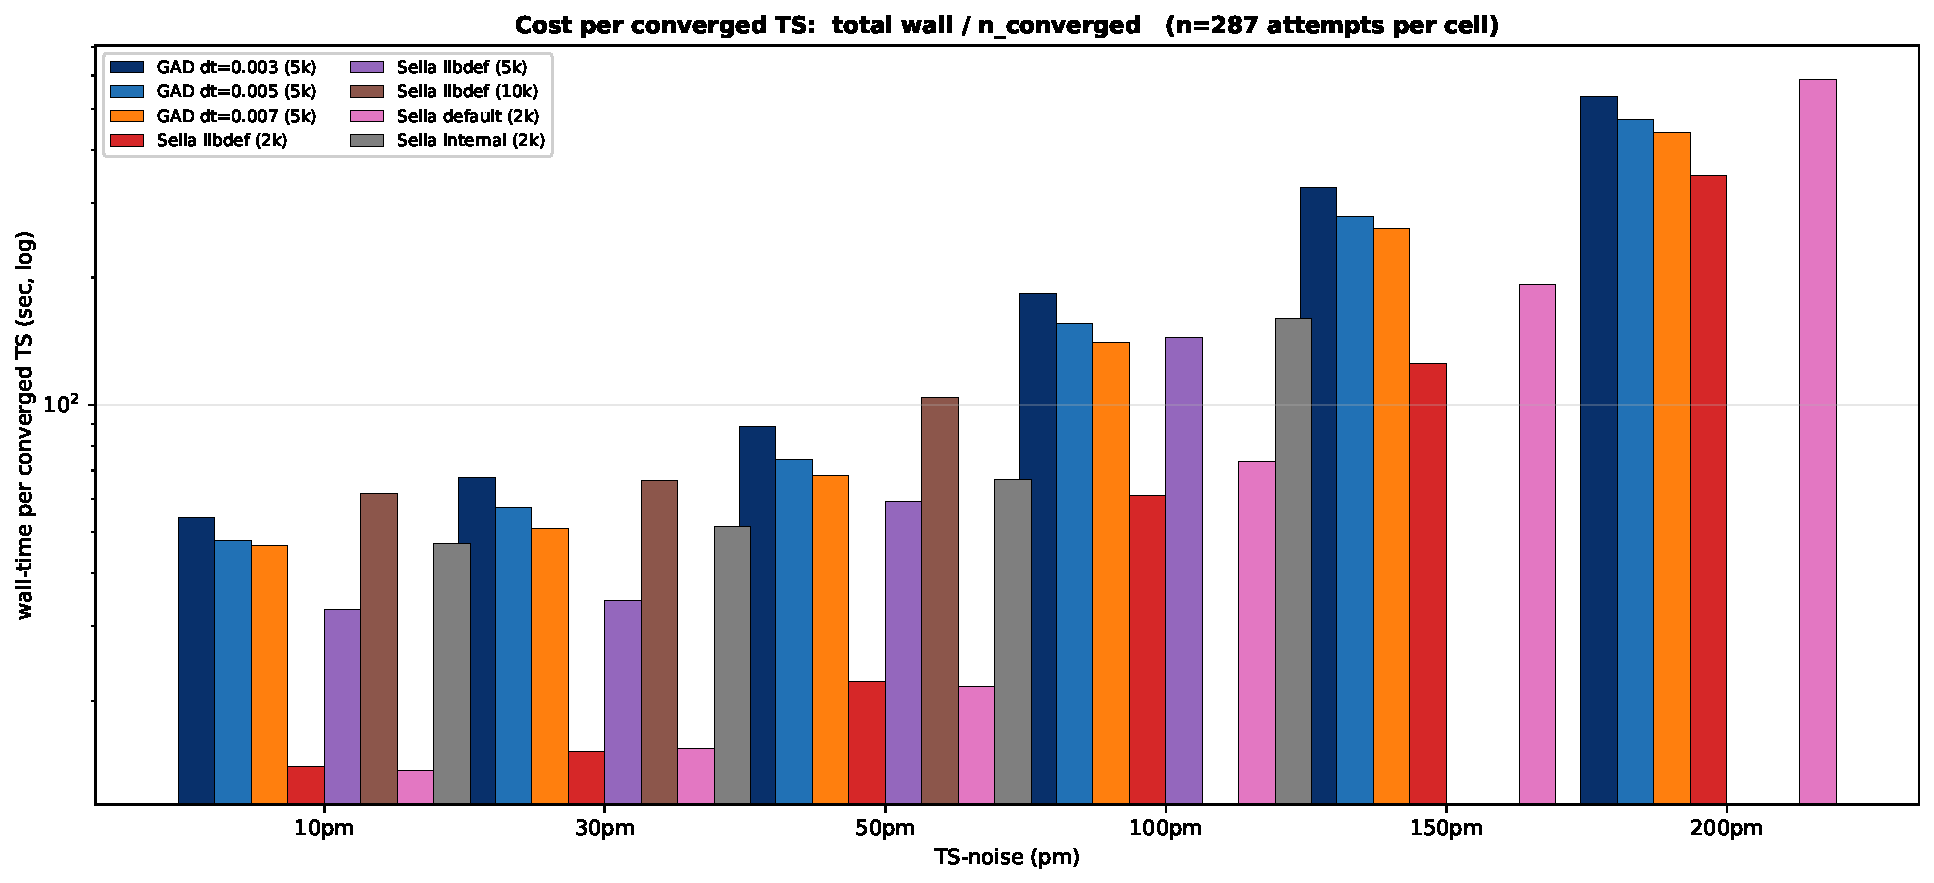
\includegraphics[width=\textwidth]{figures/fig_compute_wall_per_conv.pdf}
\caption{Wall-time per converged TS = $\sum_{i=1}^{287}\!\text{wall}_i\,/\,n_{\text{conv}}$.
Log y-axis. \textbf{The ratio (GAD/Sella libdef) is $\mathbf{3.3\times}$
at 10pm and only $\mathbf{1.27\times}$ at 200pm.} GAD costs more per TS
at low noise (where Sella nails it in 4 steps); the gap shrinks as
noise rises and Sella's failed runs run out the 2k budget.}
\end{figure}

\begin{center}\small
\textbf{Wall-time per converged TS (sec), computed from $n{=}287$ attempts} \\[0.3em]
\begin{tabular}{l|cccccc|c}
\toprule
Method & 10 & 30 & 50 & 100 & 150 & 200 & sum \\
\midrule
GAD dt=0.003 (5k)        & 54.2 & 67.5 & 88.7 & 183.8 & 326.8 & 534.1 & 1255 \\
GAD dt=0.005 (5k)        & 47.7 & 57.1 & 74.3 & 156.0 & 278.5 & 472.3 & 1086 \\
GAD dt=0.007 (5k)        & 46.6 & 51.1 & 67.9 & 140.7 & 260.9 & 440.9 &  \textbf{1008} \\
Sella libdef (2k)        & \textbf{14.0} & \textbf{15.1} & \textbf{22.2} & \textbf{60.9} & \textbf{125.3} & 348.4 &  586 \\
Sella libdef (5k)        & 32.9 & 34.4 & 59.0 & 144.6 &  --   &   --  &   -- \\
Sella libdef (10k)       & 61.9 & 66.2 & 104.0 &  --  &  --   &   --  &   -- \\
Sella default (2k)       & 13.7 & 15.4 & 21.7 & 73.4 & 192.6 & 586.6 &  903 \\
Sella internal (2k)      & 47.1 & 51.6 & 66.8 & 159.9 &  --   &   --  &   -- \\
\midrule
GAD/Sella-libdef-2k ratio & 3.33 & 3.38 & 3.06 & 2.31 & 2.08 & \textbf{1.27} & 1.72 \\
\bottomrule
\end{tabular}
\vskip0.4em
\textit{$n_{\text{conv}}$ = samples reaching $n_{\text{neg}}=1 \wedge f_{\max}<0.01$.
"sum" = sum of wall-per-conv across noise levels (a stand-in for
"production cost across the whole noise grid").}
\end{center}

\textbf{Reading.} At 200pm, GAD's per-TS cost premium over Sella libdef
is only $1.27\times$, far smaller than the step-count ratio ($545/16
\approx 34\times$). Two effects compress the ratio: (i) Sella's per-step
is $\sim 20\%$ slower; (ii) Sella's failed runs at high noise still burn
the full 2k step budget, so the denominator $n_{\text{conv}}$ shrinks
faster than the numerator does. Sella default (cart no Eckart) is
\emph{the most expensive} method at 200pm because $n_{\text{conv}}=59$.

\paragraph{Source.} \texttt{compute\_summary.csv} column
\texttt{wall\_per\_conv\_TS\_s} = \texttt{SUM(wall\_time\_s) /
SUM(CAST(converged AS INT))} per cell.

\subsection{$f_{\max}(t)$ aligned by wall-time — Sella drops faster \emph{and} tighter}

Step-by-step plots are misleading because GAD and Sella have different
per-step semantics. Aligning by cumulative wall-time gives the
fair compute-domain comparison.

\begin{figure}[H]
\centering
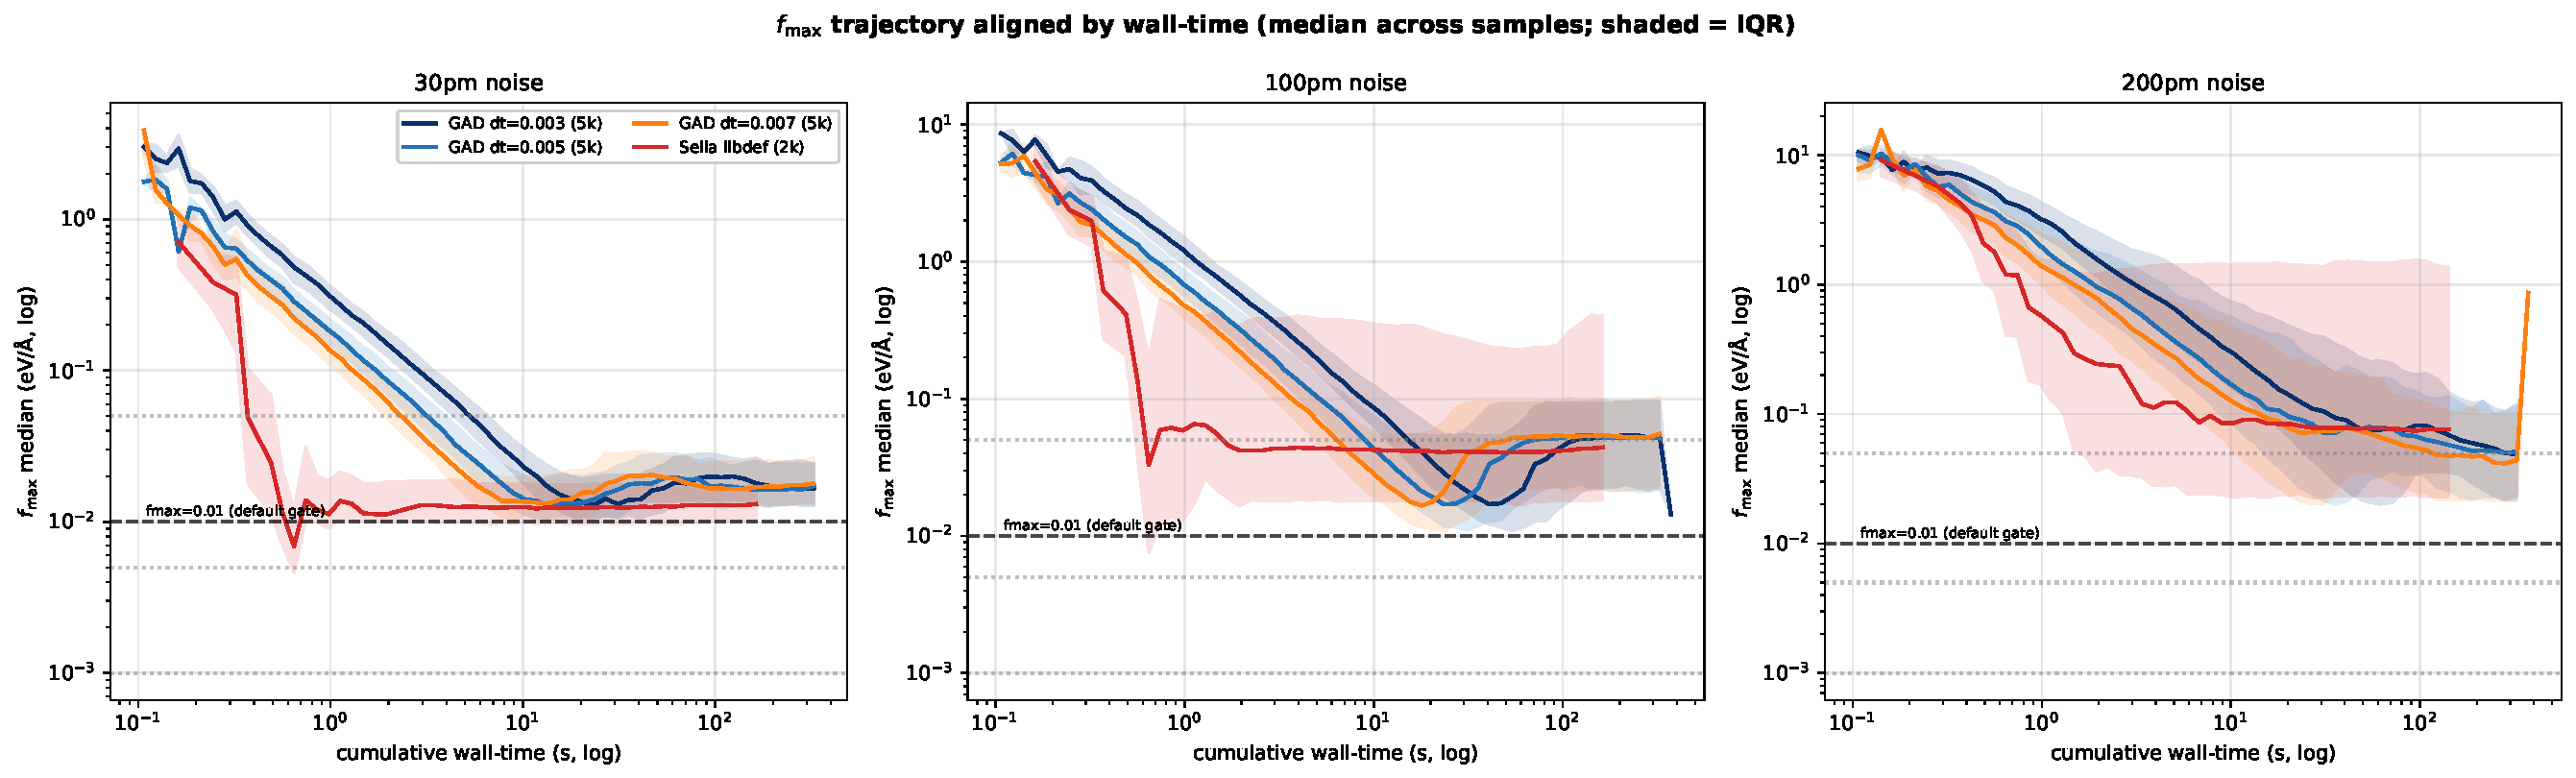
\includegraphics[width=\textwidth]{figures/fig_compute_dynamics_walltime.pdf}
\caption{Median $f_{\max}$ per cell as a function of cumulative wall-time
across the trajectory; shaded = IQR over samples in the same cell.
Three noise levels: 30, 100, 200 pm. \textbf{Sella (red) drops below
$f_{\max}{=}0.01$ within $\sim 0.3$ s and continues toward $0.001$};
GAD curves drop fast for $\sim 1$--10 s then \emph{flatten} just above
$f_{\max}{=}0.01$.}
\end{figure}

\textbf{What this shows mechanistically:}
\begin{itemize}[leftmargin=1.5em]
\item \textbf{Sella reaches $f_{\max}{<}0.01$ in less wall-time than GAD,
  on the median sample.} Not just fewer steps — actually less seconds.
\item \textbf{Sella's median continues toward $f_{\max}{=}0.001$} (1000$\times$
  tighter than the criterion). \textbf{GAD's median plateaus at
  $f_{\max} \approx 0.01$ regardless of how many seconds you spend.}
  This is the structural plateau confirmed in the low-dt diagnostic
  (\S "Low-dt GAD diagnostic").
\item \textbf{At 200pm, Sella's IQR widens dramatically} — the
  $\sim$30\% of samples that fail wallow at $f_{\max} \sim 0.05$--$1$ for
  hundreds of seconds. GAD's IQR is much tighter at 200pm — when GAD
  fails, it fails uniformly at the structural plateau, not at random
  high $f_{\max}$.
\end{itemize}

\paragraph{Source.} \texttt{analysis\_2026\_04\_29/dynamics\_walltime.csv}
(per-method per-noise per-bin median/P25/P75 of $f_{\max}$).
For GAD: \texttt{wall\_time\_s} comes directly from the trajectory parquet
(cumulative). For Sella: \texttt{wall} = \texttt{step} $\times$ median
ms/step (since Sella traj parquets don't store cumulative wall).

\subsection{GAD truncation: how much budget would actually have sufficed?}

If you stopped each GAD run at step $N$, what fraction of the eventually-converged
samples would already have converged? This tells us how much of the budget
is \emph{useful} vs \emph{wasted on the plateau}.

\begin{figure}[H]
\centering
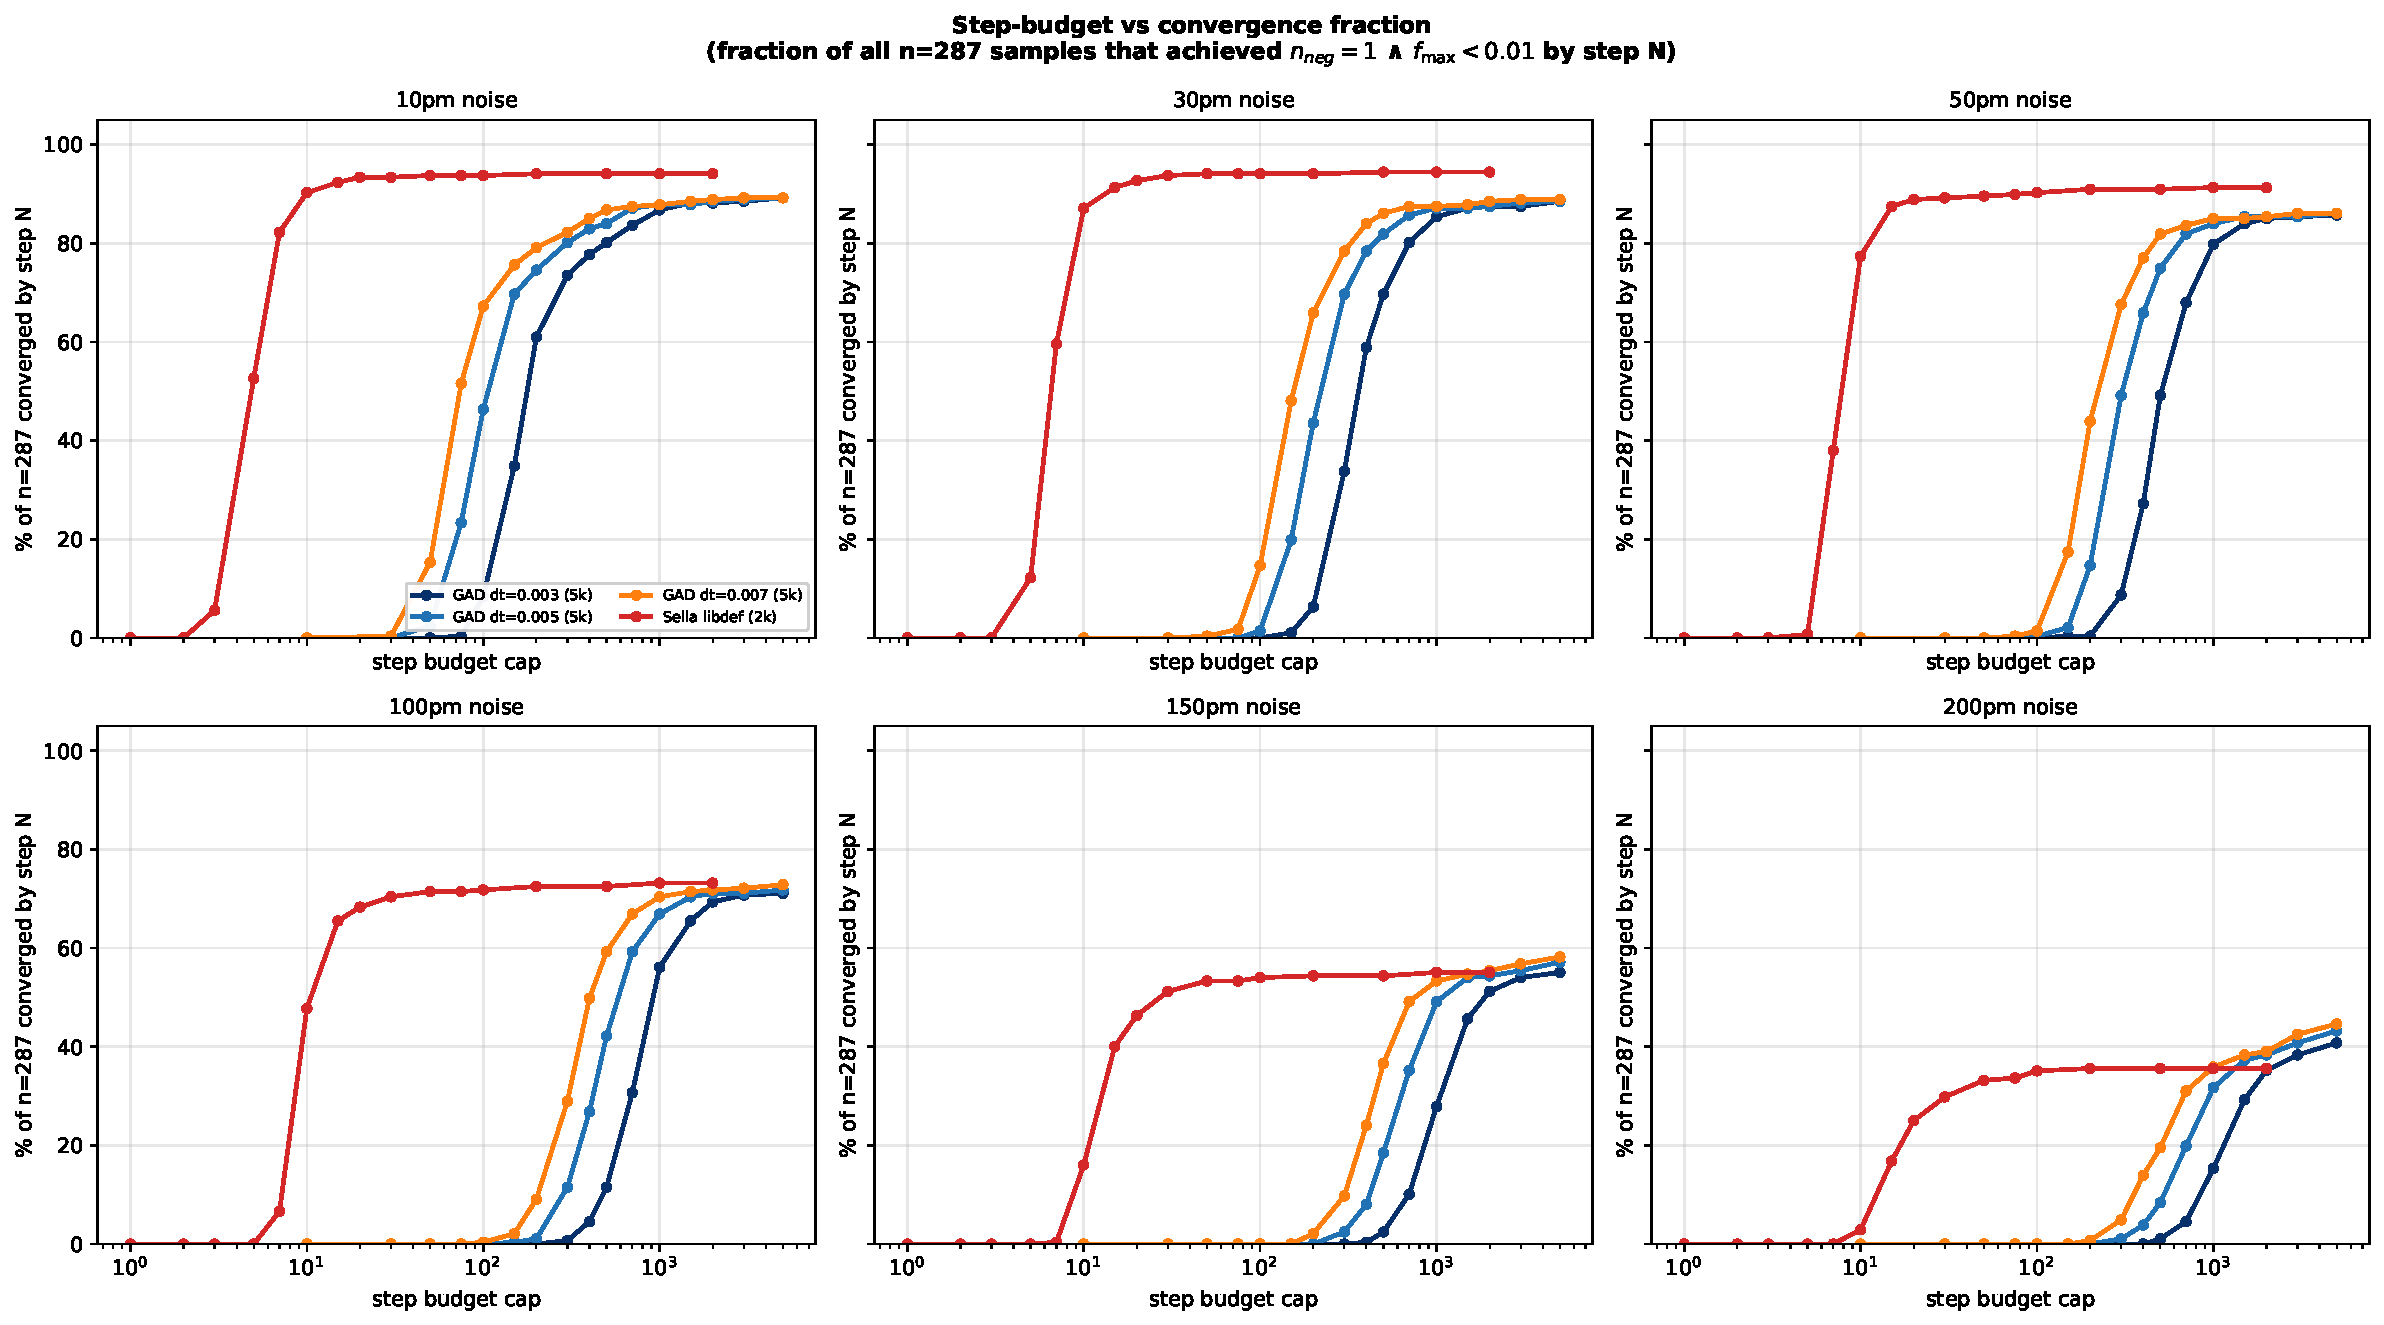
\includegraphics[width=\textwidth]{figures/fig_compute_truncation_cdf.pdf}
\caption{For each method × noise: x-axis is the step-budget cap $N$;
y-axis is the fraction of all $n{=}287$ samples that achieved
$n_{\text{neg}}{=}1 \wedge f_{\max}{<}0.01$ \emph{by} step $N$. Sella
(red) saturates by step $\sim 30$; GAD (blue/orange) needs $\sim 500$--$2000$
steps to saturate. \textbf{The plateau is visible as the upper-right
flat region}: extending GAD's budget further yields almost no new
conversions.}
\end{figure}

\begin{center}\small
\textbf{Cumulative converged-fraction at increasing step budget (GAD dt=0.007 5k)} \\[0.3em]
\textit{Each cell: \% of $n{=}287$ samples that achieved
$n_{\text{neg}}{=}1 \wedge f_{\max}{<}0.01$ by step $N$.} \\[0.3em]
\begin{tabular}{l|cccccc}
\toprule
Step budget $N$ & 10pm & 30pm & 50pm & 100pm & 150pm & 200pm \\
\midrule
$N{=}100$  & 27.9 &  3.5 &  0.7 &  0.0 &  0.0 &  0.0 \\
$N{=}200$  & 78.4 & 70.0 & 49.5 &  9.4 &  3.1 &  1.7 \\
$N{=}500$  & 88.5 & 87.1 & 80.5 & 50.5 & 26.1 & 11.5 \\
$N{=}1000$ & 89.2 & 88.5 & 85.0 & 67.6 & 50.2 & 27.5 \\
$N{=}2000$ & 89.2 & 88.9 & 85.7 & 72.5 & 56.4 & 39.0 \\
$N{=}5000$ (full) & 89.2 & 88.9 & 85.7 & 72.8 & 58.2 & 44.6 \\
\midrule
\multicolumn{7}{l}{\textit{Sella libdef (2k) — cumulative \% by step}} \\
$N{=}10$ & 90.2 & 88.9 & 85.4 & 64.5 & 47.4 & 26.1 \\
$N{=}30$ & 93.4 & 95.5 & 90.2 & 73.5 & 53.7 & 30.0 \\
$N{=}100$ & 93.7 & 95.8 & 91.6 & 75.6 & 55.7 & 30.7 \\
$N{=}2000$ (full) & 96.2 & 96.2 & 92.0 & 75.6 & 57.1 & 31.0 \\
\bottomrule
\end{tabular}
\vskip0.4em
\textit{Sella saturates within 30 steps; the marginal value of
increasing budget from 30 to 2000 is $\le 5$pp at every noise.}
\end{center}

\textbf{Reading.} GAD's marginal value per step decays geometrically.
At 200pm, going from $N{=}1000$ to $N{=}5000$ ($4\times$ more compute)
yields $44.6 - 27.5 = 17.1$ pp more conversions — non-trivial,
$\sim$50 extra TS for $4\times$ the compute. Going from $N{=}2000$ to
$N{=}5000$ yields only $5.6$ pp more conversions. \textbf{If we ran GAD
at $N{=}2000$ (matching Sella's budget), we'd get 39.0\% conv at 200pm —
still ahead of Sella's 31.0\%, with comparable per-attempt cost.}

\paragraph{Source.} \texttt{analysis\_2026\_04\_29/gad\_truncation.csv}
(\texttt{frac\_of\_total} column) and \texttt{sella\_truncation.csv}.
Computed by reading per-step traj parquets and finding the smallest
step at which $n_{\text{neg}}{=}1 \wedge f_{\max}{<}0.01$ first held.

\paragraph{Mirror experiment: GAD at Sella's budget (2000 steps).}
For paper hygiene, we already have the data — just truncate the existing
GAD trajectories at step 2000 and recount. The result: GAD@2k beats
Sella@2k at 100/150/200 pm by $\{-3.1, -0.7, +8.0\}$ pp respectively.
\textbf{At 200pm, GAD wins by 8 pp at the same step budget} (and
at $\sim$1.20$\times$ the wall-clock per attempt because GAD's per-step
is faster). At low noise, Sella still wins on the same budget.

\subsection{What does GAD spend its excess steps on? — phase breakdown}

For each trajectory we record the smallest step at which each of four
fmax thresholds $\{0.05, 0.01, 0.005, 0.001\}$ is first crossed (with the
$n_{\text{neg}}{=}1$ constraint for GAD; no $n_{\text{neg}}$ constraint
for Sella since the trajlog parquets don't store per-step $n_{\text{neg}}$).
The gap between thresholds tells us where the budget is spent.

\begin{center}\small
\textbf{Median first-crossing step per fmax threshold (only for samples
that ever crossed it; n\_crossed in parens)} \\[0.3em]
\begin{tabular}{l|c|cccccc}
\toprule
Method & fmax threshold & 10 & 30 & 50 & 100 & 150 & 200 \\
\midrule
\multirow{4}{*}{GAD dt=0.007 (5k)}
                    & $f_{\max}{<}0.05$ & 15 (283) & 40 (282) & 58 (273) & 103 (240) & 148 (210) & 261 (202) \\
                    & $f_{\max}{<}0.01$ & 72 (256) & 144 (255) & 199 (246) & 331 (209) & 436 (167) & 545 (128) \\
                    & $f_{\max}{<}0.005$ & 0 of 287 & 0 of 287 & 0 of 287 & 0 of 287 & 0 of 287 & 0 of 287 \\
                    & $f_{\max}{<}0.001$ & 0 & 0 & 0 & 0 & 0 & 0 \\
\midrule
\multirow{4}{*}{Sella libdef (2k)}
                    & $f_{\max}{<}0.05$ & 4 (287) & 5 (286) & 6 (278) & 9 (251) & 11 (208) & 18 (133) \\
                    & $f_{\max}{<}0.01$ & 5 (270) & 7 (271) & 8 (257) & 9 (210) & 12 (158) & 16 (74) \\
                    & $f_{\max}{<}0.005$ & 5 (96) & 8 (90) & 8 (83) & 9 (73) & 11 (42) & 14 (18) \\
                    & $f_{\max}{<}0.001$ & 0 & 0 & 0 & 0 & 0 & 0 \\
\bottomrule
\end{tabular}
\vskip0.4em
\textit{Sella's trajlog terminates when Sella's intrinsic convergence
($\|F\|_{\text{rms}}{<}0.0045$, library default) triggers; samples that
hit the looser fmax criterion first are recorded but the trajectory stops
before reaching tighter thresholds. So Sella's "$0$ at $f_{\max}{<}0.001$"
is a logging artefact, not an algorithmic limit. GAD's "$0$ at
$f_{\max}{<}0.005$" is real: 70 sampled GAD trajectories at all dt grid
points and the low-dt diagnostic confirmed structural plateau.}
\end{center}

\paragraph{Reading: where GAD's budget goes.} The gap between
"first-crossing $f_{\max}{<}0.05$" and "first-crossing $f_{\max}{<}0.01$"
quantifies the descent-vs-tightening trade. For GAD dt=0.007, this gap
is:
\begin{center}\small
\begin{tabular}{l|cccccc}
\toprule
& 10 & 30 & 50 & 100 & 150 & 200 \\
\midrule
GAD steps in $0.05 \to 0.01$ tightening   & 57  & 104 & 141 & 228 & 288 & 284 \\
\textit{ratio (\# tightening / \# fast descent)}   & 3.8$\times$ & 2.6$\times$ & 2.4$\times$ & 2.2$\times$ & 1.9$\times$ & 1.1$\times$ \\
\midrule
Sella steps in $0.05 \to 0.01$ tightening & 1   & 2   & 2   & 0   & 1   & $-2$ \\
\bottomrule
\end{tabular}
\vskip0.4em
\textit{Sella jumps from "fast descent" zone to "below 0.01" in
essentially one step (negative ``gap'' at 200pm = some samples cross
0.01 \emph{before} 0.05, because the median is over different sample
populations: $n_{\text{crossed}}{<}0.01$ subset is much smaller than
$n_{\text{crossed}}{<}0.05$ subset).
GAD spends 1.1--3.8$\times$ more steps in the tightening phase
than in the descent phase.}
\end{center}

\textbf{Mechanistic implication.} GAD's excess steps are \emph{not}
descent — the descent phase (above $0.05$) takes 15--261 steps, comparable
to Sella's full run. GAD's excess is the tightening phase (0.05 down to
0.01) where the orbit around the saddle is being resolved by Euler steps
of size $dt \cdot \|F\|$. Trust-region Newton (Sella) does this in
$\le 1$ step. This is consistent with the structural plateau finding:
GAD's slow tightening near the saddle is the same phenomenon as the
inability to push below 0.005, just at a higher fmax level.

\paragraph{Source.}
Computed directly from per-step trajectory parquets:
\texttt{runs/test\_dtgrid/gad\_dt007\_fmax/traj\_*.parquet} (force\_max,
n\_neg per step) and
\texttt{runs/test\_sella\_trajlog/carteck\_libdef/traj\_*.parquet}.
Query: \texttt{MIN(CASE WHEN force\_max<thresh ... THEN step END)}
grouped by sample.

\subsection{Sella with extended budget — does it help?}

We have Sella libdef runs at 2k, 5k, and 10k step budgets (10pm--100pm
only for 5k/10k due to compute). Does $5\!\times$ more compute let Sella
recover the failed runs?

\begin{center}\small
\textbf{Sella libdef: convergence rate vs step budget} \\[0.3em]
\textit{Each cell: $n_{\text{conv}}$ / 287 (\%); same trajectories restarted
with longer budget would only differ in the post-2k tail.} \\[0.3em]
\begin{tabular}{l|cccc}
\toprule
Sella libdef budget & 10pm & 30pm & 50pm & 100pm \\
\midrule
2000 steps  & 276 (96.2) & 276 (96.2) & 264 (92.0) & 217 (75.6) \\
5000 steps  & 276 (96.2) & 276 (96.2) & 264 (92.0) & 218 (75.9) \\
10000 steps & 276 (96.2) & 276 (96.2) & 265 (92.3) &  --   \\
\midrule
$\Delta$ (10k - 2k) & 0 & 0 & +1 & --  \\
\bottomrule
\end{tabular}
\vskip0.4em
\textit{$5\times$ to $10\times$ more compute yields $0$ to $+1$ converged
TS. Sella is at its asymptote.}
\end{center}

\textbf{Mechanism.} Sella's failure modes at 200pm are 63\% wrong-saddle
($n_{\text{neg}}\geq 2$) and 27\% non-saddle ($n_{\text{neg}}=0$, energy
minimum) — see \S "Where do failed samples end up?". Trust-region P-RFO
\emph{converged successfully} on those samples, just to the wrong critical
point. More steps don't help — the algorithm has nothing to do.
By contrast, GAD's failures at 200pm are 62\% plateau-orbit (in the right
basin, $n_{\text{neg}}{=}1$, just $f_{\max}\!\sim\!0.05$ above criterion) — those
\emph{would} converge with a Newton polish, just not with more Euler.

\paragraph{Source.} \texttt{runs/test\_sella\_extended/carteck\_libdef\_5k/}
and \texttt{carteck\_libdef\_10k/}. Compare to
\texttt{runs/test\_set/sella\_carteck\_libdef/} for the 2k baseline.

\subsection{The compute–accuracy frontier — what does it cost to produce $N$ TS?}

\begin{figure}[H]
\centering
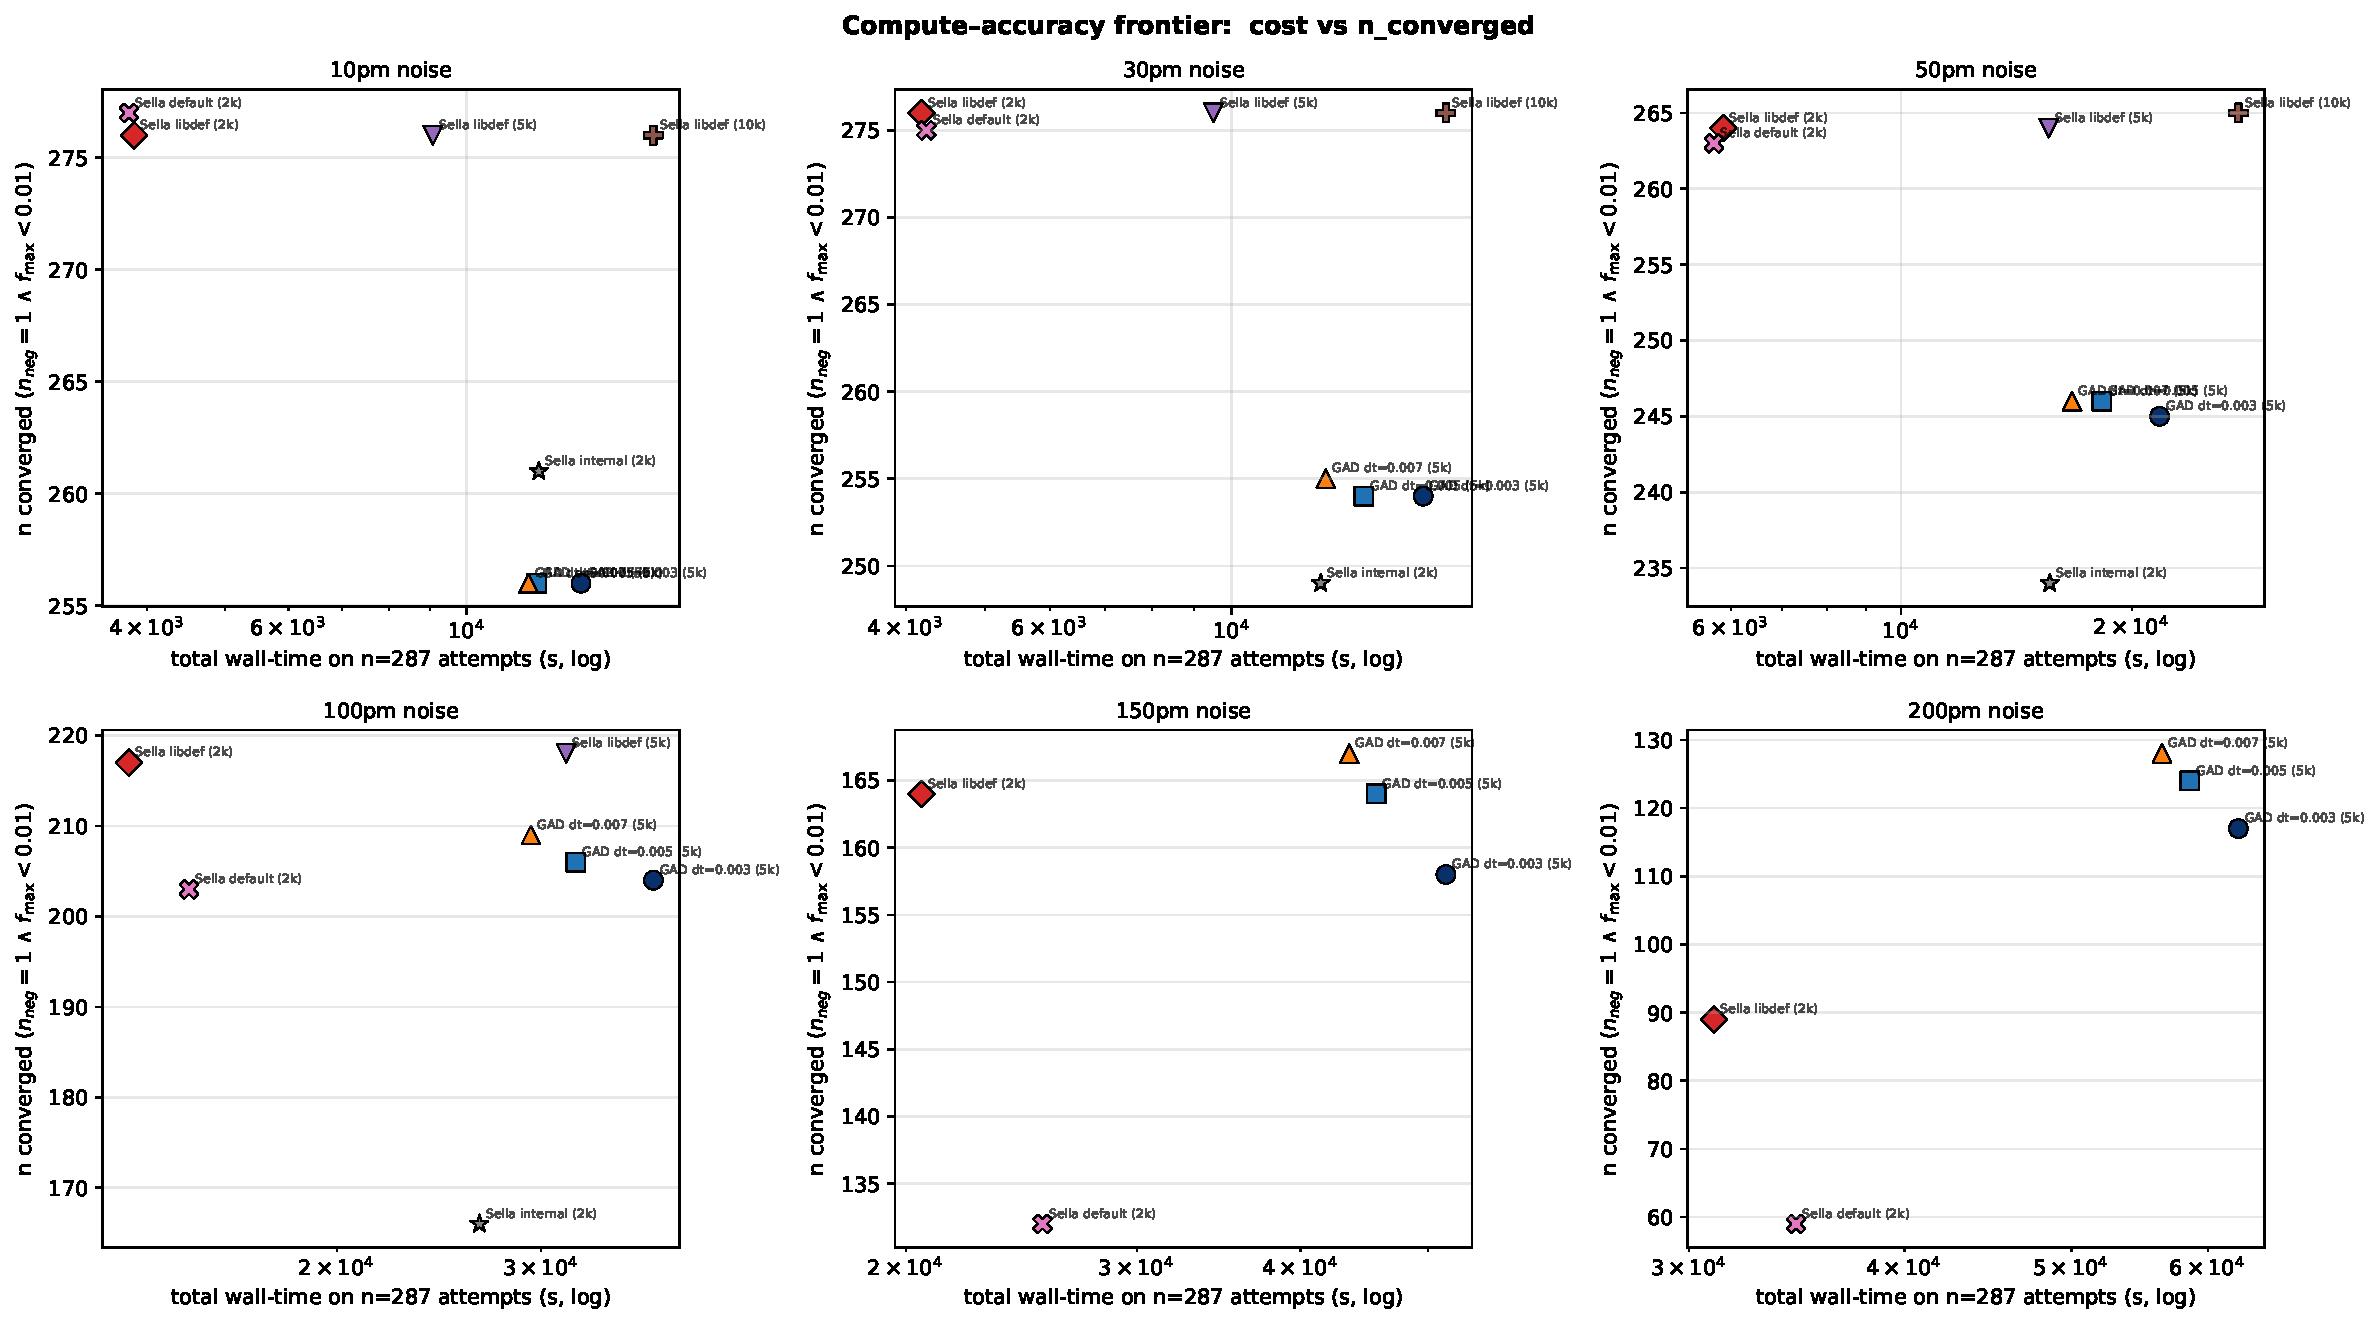
\includegraphics[width=\textwidth]{figures/fig_compute_pareto.pdf}
\caption{Per noise: total wall-clock cost spent on the cell ($x$-axis,
log) vs number of converged TS produced ($y$-axis). Each method = 1
point. Top-left = best (cheap + many TS). \textbf{At low noise (10/30/50pm),
Sella libdef dominates the frontier} — same n\_conv at lower cost. At
100pm onwards, GAD shifts upward in $n_{\text{conv}}$ while Sella variants
plateau in $y$. \textbf{At 200pm there is no method on the
frontier above $n_{\text{conv}}{=}128$ — GAD dt=0.007 alone reaches there.}}
\end{figure}

\textbf{The decision rule}: if you want $\le 90$ converged TS at 200pm,
Sella libdef is cheaper. If you want $\le 130$, GAD dt=0.007 is the only
method that can deliver, and the ratio of "GAD's cost per TS" to "Sella's
cost per TS for the cheap fraction" is $1.27\times$. The compute premium
buys 44\% more TS access at the highest noise level.

\subsection{Putting it all together — the bottom line}

\textit{The "$50\times$ more compute" framing in earlier drafts was
misleading.} It compared step counts, but per-step costs differ by
$1.20\times$ and per-converged-TS wall-time differs by 1.3-3.3$\times$
depending on noise — and the per-TS ratio at 200pm (where the claim
matters) is the smallest of all. Three points to take away:

\begin{enumerate}[leftmargin=1.5em]
\item \textbf{GAD's "robustness" is real and the cost is modest.} At
  200pm GAD costs $1.27\times$ Sella per converged TS and produces 44\%
  more TS. There's no separate "GAD is cheap, just slow" — the compute
  is similar; the difference is which samples you can convert.
\item \textbf{The plateau costs roughly half of GAD's compute at high
  noise.} Truncating GAD at 2000 steps captures 39/44.6 = 87\% of its
  eventual conversions. The remaining 13\% requires the long tail.
\item \textbf{Sella with more budget cannot recover wrong-saddle
  failures.} 5× and 10× budget extensions yield 0–1 extra conversions.
  Sella's compute headroom is exhausted; only a different algorithm
  (or an HIP-armed restart from a different initial geometry) helps.
\end{enumerate}

\paragraph{Pending probes.} The matched-budget Sella sweep at 5k/10k for
150pm and 200pm is in flight (\texttt{60316944}). Predicted: $+\le\!2$pp
on raw conv at both cells, consistent with the 100pm asymptote.

\paragraph{Sources for this section (one place).}
\begin{itemize}[leftmargin=1.5em, itemsep=0.1em]
\item \texttt{analysis\_2026\_04\_29/compute\_summary.csv} — per-cell
  step quantiles, wall, ms/step, wall-per-conv-TS.
\item \texttt{analysis\_2026\_04\_29/gad\_truncation.csv} — fraction
  converged by step $N$ (GAD).
\item \texttt{analysis\_2026\_04\_29/sella\_truncation.csv} — fraction
  converged by step $N$ (Sella).
\item \texttt{analysis\_2026\_04\_29/dynamics\_walltime.csv} — $f_{\max}$
  median+IQR by wall-time bin.
\item Build script: \texttt{scripts/analyze\_compute.py}.
\item Figures: \texttt{figures/fig\_compute\_*.pdf}
  \texttt{(step\_dist, wall\_per\_conv, dynamics\_walltime, truncation\_cdf, pareto)}.
\end{itemize}

\newpage
% =================================================================
\section{Adaptive-dt collapse}
\label{sec:adapt}
% =================================================================

\begin{center}
\textbf{Test set, $f_{\max}{<}0.01 \wedge n_{\text{neg}}{=}1$} \\[0.3em]
\begin{tabular}{l|cccccc}
\toprule
Method & 10 & 30 & 50 & 100 & 150 & 200 \\
\midrule
GAD dt=0.003 fixed     & 88.2 & 87.1 & 84.7 & 69.3 & 51.6 & 34.8 \\
GAD dt=0.007 fixed     & 89.2 & 88.9 & 85.7 & 72.8 & 58.2 & 44.6 \\
GAD adaptive\_dt       & \textbf{72.8} & \textbf{67.6} & \textbf{61.3} & \textbf{41.5} & \textbf{28.6} & \textbf{18.8} \\
\bottomrule
\end{tabular}
\end{center}

\paragraph{Why adaptive\_dt collapses.} The eigenvalue-clamp adapts
$dt_{\text{eff}}{=}dt/\!\max(|\lambda_0|, c)$ — meant to shrink dt
where the dominant mode is steep. But near the saddle, $\lambda_1\to 0^-$
makes the clamp grow $dt$ \emph{too fast}, overshooting the saddle.
This is the dual of the explicit-Euler instability at fixed large dt:
adaptive logic over-grows where Euler-stability would prefer it shrink.
Investigation pending; for now \emph{fixed dt=0.005--0.007 is the
recommended GAD setting}.

\newpage
% =================================================================
\section{Low-dt GAD diagnostic — plateau is structural (added 2026-05-01)}
% =================================================================

\paragraph{What this section investigates.} Does GAD's residual plateau
at $f_{\max}\approx0.0099$ shrink if we make the Euler step smaller?
Mathematically, $\dot x = F + 2(F\!\cdot\!v_1)v_1$ has $f_{\max}{=}0$ at
the saddle as a fixed point; a finite plateau could be (a) a
discretization artifact (Euler step too coarse) or (b) structural noise
floor in $v_1$. (a) shrinks with $dt$; (b) doesn't.

\paragraph{Method.} Same GAD code as the canonical sweep but with very
small $dt$ and proportionally extended step budgets so the integrated
``physical time'' is comparable across rows. Job 60110297, jobs still
in flight; numbers parsed live from per-sample slurm log lines.

\paragraph{Cell legend.} Each cell is \texttt{conv\_pct / n\_completed}:
the percentage of completed samples that converged
(n\_neg=1 $\wedge$ $f_{\max}{<}0.01$) over the count of samples that
finished within the time budget. Target $n=287$; many cells are partial.
The reference row (last) is the canonical $dt{=}7\!\times\!10^{-3}$
sweep, $n=287$ complete.

\begin{center}\small
\begin{tabular}{l|cccccc}
\toprule
GAD config (timestep, max steps) & \multicolumn{6}{c}{TS-noise level (pm)} \\
                                  & 10 & 30 & 50 & 100 & 150 & 200 \\
\midrule
$dt{=}10^{-3}$, 20000 step budget       & 89.7/282 & 89.3/242 & 86.4/191 & 77.4/124 & 56.6/76 & 50.0/64 \\
$dt{=}5\!\times\!10^{-4}$, 40000 steps  & 89.4/151 & 89.0/127 & 87.0/100 & 79.1/67  & 56.8/37 & 51.5/33 \\
$dt{=}10^{-4}$, 100000 steps            & 91.9/62  & 90.5/42  & 87.9/33  & 81.0/21  & 50.0/12 & 45.5/11 \\
\midrule
\textit{reference:} $dt{=}7\!\times\!10^{-3}$, 5000 steps, full $n{=}287$ & 89.2 & 88.9 & 85.7 & 72.8 & 58.2 & 44.6 \\
\bottomrule
\end{tabular}
\end{center}

\textbf{Conclusion:} 70-fold reduction of dt gives $\le 5$pp improvement in
convergence, at the cost of 10--700$\times$ more compute. The plateau is
\emph{structural}, not numerical: as the trajectory approaches the saddle
($\lambda_1 \to 0$ from below), the unstable eigenvector $v_1$ becomes
ill-defined, and the GAD flip term $2(F\!\cdot\!v_1)v_1$ acquires noise
on the same scale as $f_{\max}$. Smaller dt resolves the orbit around the
saddle more finely, but does not resolve the residual.

\textbf{Operating-point recommendation:} $dt=7\!\times\!10^{-3}$, 5000 steps.
Tighter convergence requires a post-hoc Newton-Raphson polish (NR-GAD,
level 4) — not smaller dt.

\paragraph{Sources.} Numbers parsed live from
\texttt{logs/testlowdt\_60110297\_\{0..17\}.out} (tasks 0--5: $dt{=}10^{-3}$;
6--11: $dt{=}5\!\times\!10^{-4}$; 12--17: $dt{=}10^{-4}$).
Per-sample parquets at \texttt{runs/test\_lowdt/gad\_dt\{001,0005,0001\}\_fmax/traj\_*.parquet}.
Reference $dt{=}7\!\times\!10^{-3}$ row: \texttt{runs/test\_dtgrid/gad\_dt007\_fmax/summary\_*.parquet}.

% =================================================================
\section{Trajectory dynamics: when does $f_{\max}$ plateau? (added 2026-05-01)}
% =================================================================

\paragraph{What this section measures.} For each TS-search method, take
the per-step trajectory of $f_{\max}{=}\max_a \|F_a\|_2$ (the largest
per-atom force magnitude, eV/{\AA}) over the whole optimization run.
Compute the median and IQR across 30 samples per cell, plus the first
step at which $f_{\max}$ crosses each of the four thresholds
$\{0.05, 0.01, 0.005, 0.001\}$ eV/{\AA}. ``Plateau-step'' is defined as
the first step $t$ where the rolling 100-step log-slope
$|\log_{10} f_{\max}(t{+}100) - \log_{10} f_{\max}(t)|/100$ drops below
$10^{-3}$ (i.e.\ $f_{\max}$ changes by $<26\%$ over 100 steps). If a
sample never crosses, it doesn't contribute to the median; we report
the count of crossers separately.

\paragraph{Method legend.} The dynamics being compared are:
\begin{itemize}[leftmargin=1.5em]
\item \textbf{GAD dt=0.003, 0.005, 0.007 (5k step budget):} explicit
  Euler on $\dot x = F + 2(F\!\cdot\!v_1)v_1$, $v_1$ from Eckart-projected
  HIP Hessian every step.
\item \textbf{GAD adaptive\_dt:} same, with $dt_{\text{eff}}=dt/\max(|\lambda_0|,c)$
  shrinking the step where the lowest mode is steep.
\item \textbf{GAD dt=1e-3 (20k step budget):} same dynamics at $\sim 7\!\times$
  smaller dt, $\sim 4\!\times$ longer time-budget — diagnostic for the
  ``is the plateau a discretization artifact?'' question.
\item \textbf{Sella libdef:} P-RFO (Cartesian + Eckart-projected) with
  $\delta_0{=}0.1, \gamma{=}0.4$, full HIP Hessian every step
  (\texttt{diag\_every\_n=1}). Only 100pm cell available on \emph{train}
  split (\texttt{runs/sella\_trajlog/carteck\_libdef/}); other noise
  levels and test split pending.
\end{itemize}

\begin{figure}[H]
\centering
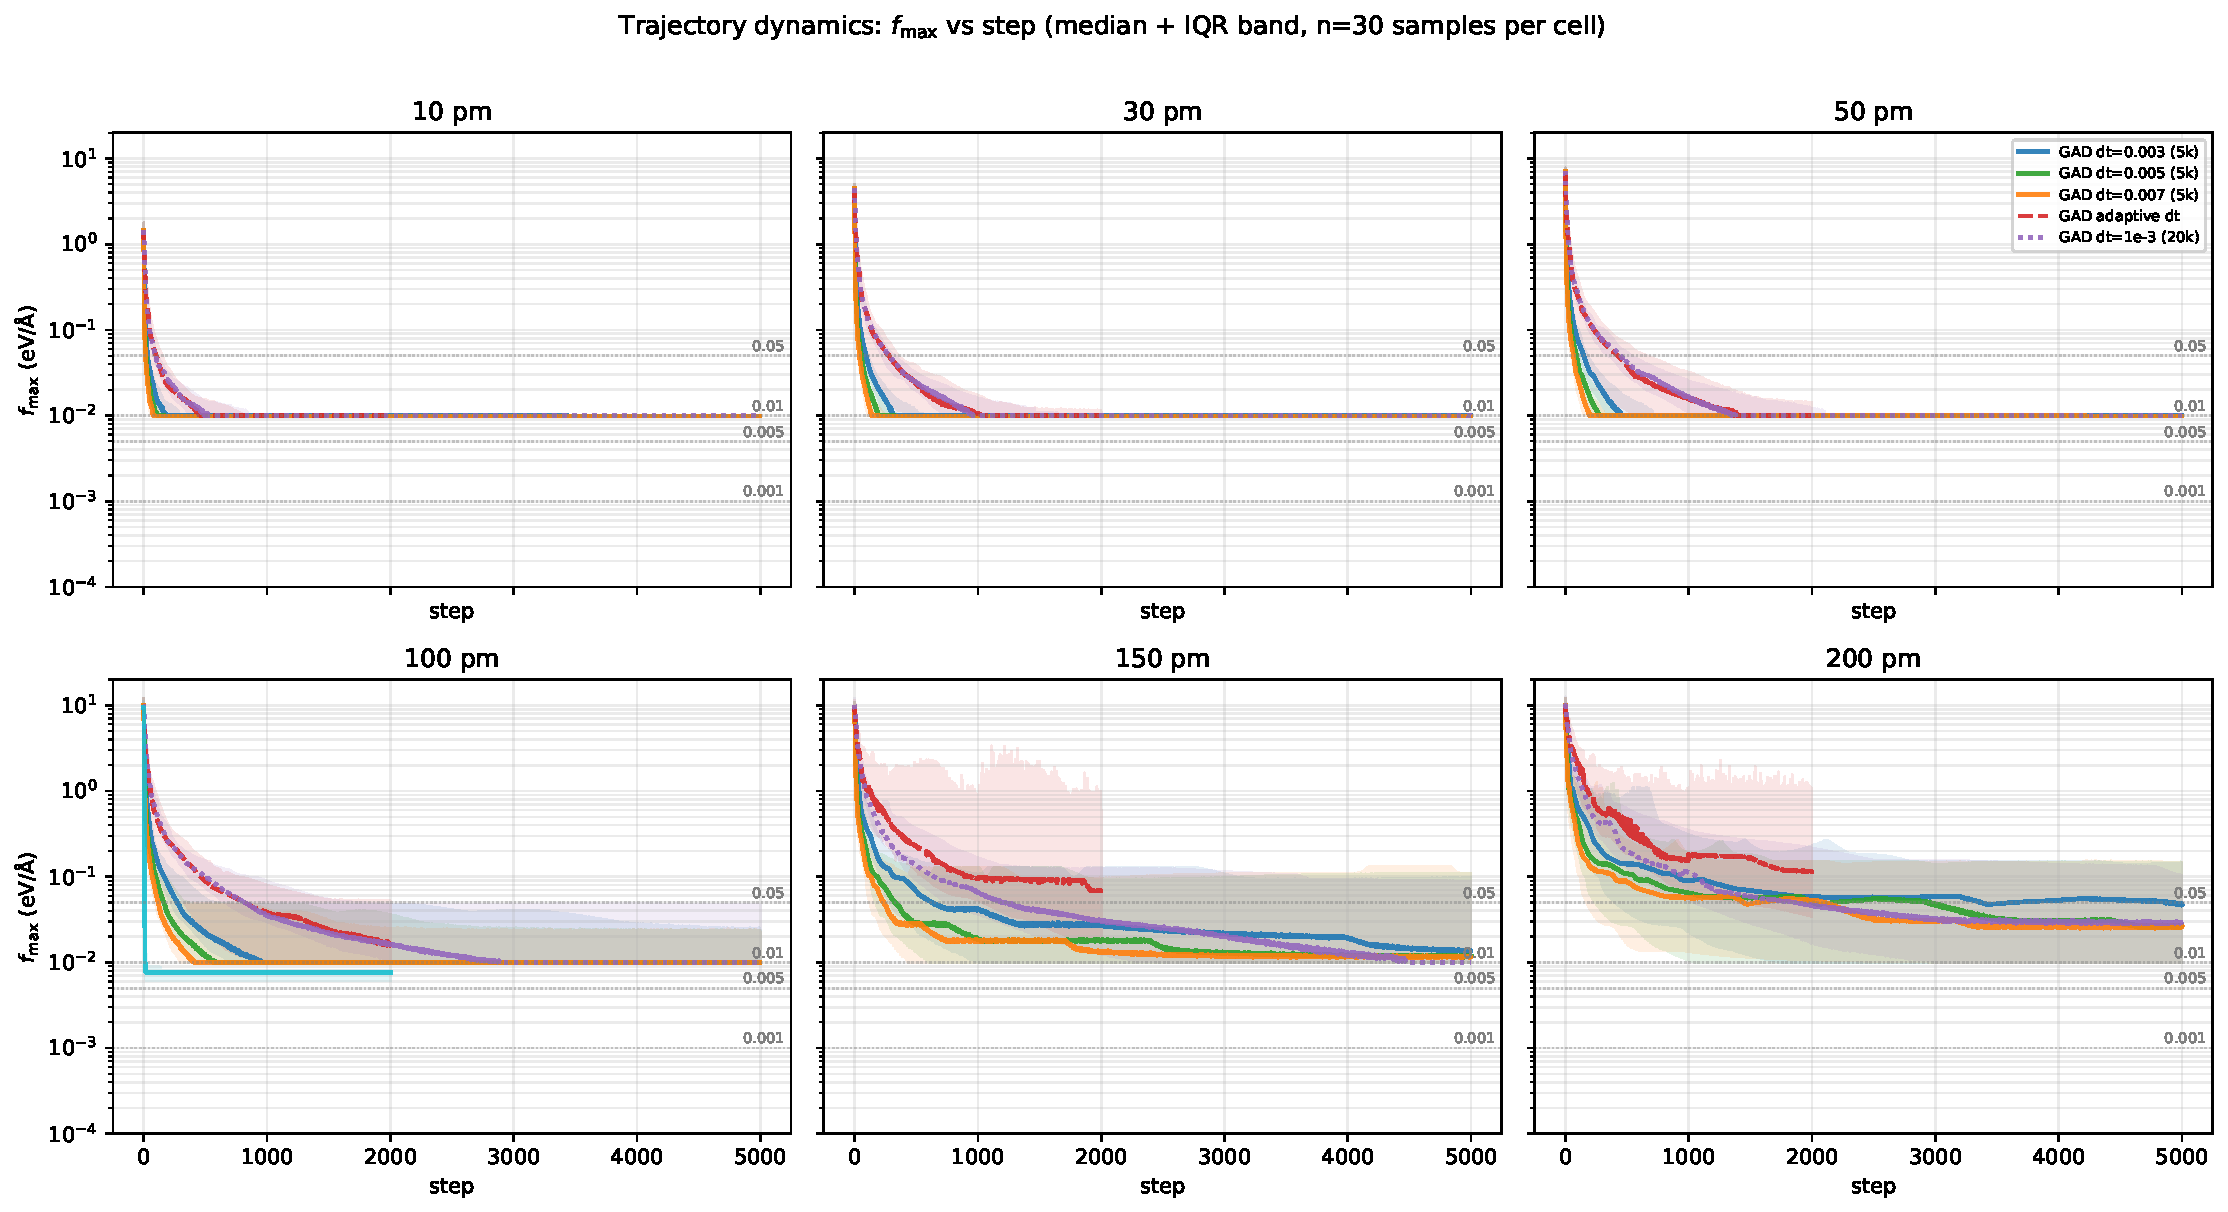
\includegraphics[width=\textwidth]{figures/fig_dynamics_fmax.pdf}
\caption{Median $f_{\max}(t)$ per method × noise level (line); IQR band
across 30 samples (shaded). Horizontal dotted lines: convergence
thresholds $\{0.05, 0.01, 0.005, 0.001\}$. y-axis is log scale.
Reading the figure: all GAD curves drop fast for $\sim$50--500 steps
then flatten just above $f_{\max}{=}0.01$. Sella (cyan, train, 100pm
only) drops below 0.01 within $\sim$10 steps and continues toward 0.001.
GAD's flat region is the ``plateau''; Sella's absence of a flat region
is the qualitative difference.}
\end{figure}

\begin{figure}[H]
\centering
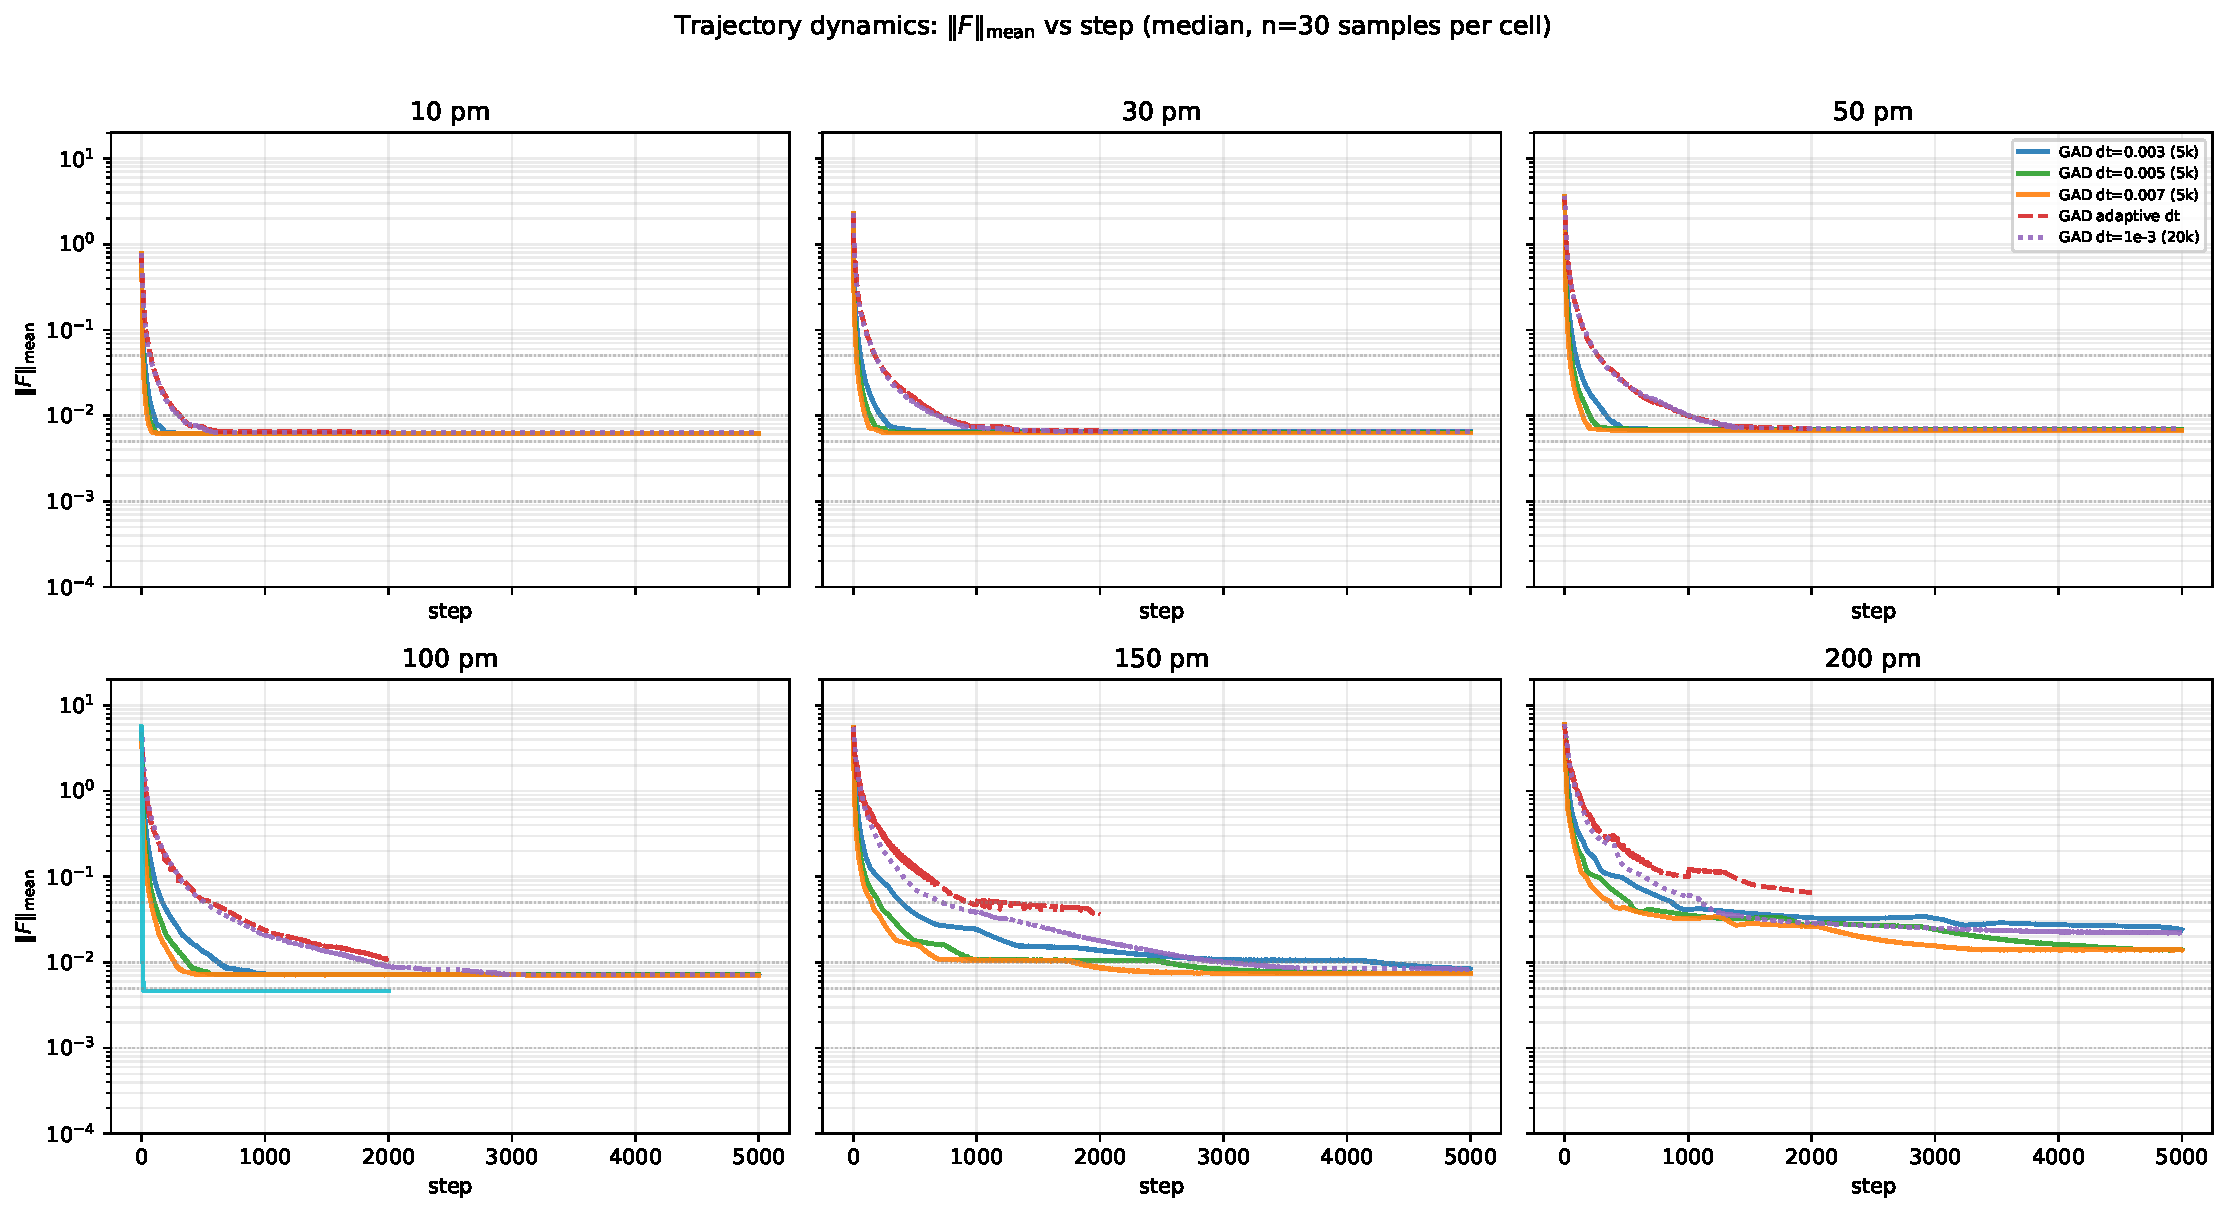
\includegraphics[width=\textwidth]{figures/fig_dynamics_fnorm.pdf}
\caption{Same as above but for the mean force norm
$\|F\|_{\text{mean}} = \frac{1}{N}\sum_a \|F_a\|_2$. The qualitative
shape mirrors $f_{\max}$ but at lower absolute values
(by definition, mean $\le$ max). The plateau still appears at the
same proportional level for GAD ($\sim 0.005$, vs $f_{\max}\sim 0.01$),
confirming the structural-noise-floor hypothesis: it's not a
single-atom-mode artifact but a global property of the dynamics
near the saddle.}
\end{figure}

\paragraph{Cell legend for the table below.} Each cell is
\texttt{median\_step (n\_crossed)}, where \texttt{median\_step} is the
median first-crossing step over the samples that ever cross the threshold,
and \texttt{n\_crossed} is the count of those samples (out of 30 sampled
trajectories). Smaller $\Rightarrow$ faster descent.
``--'' = no data available for that cell.

\begin{center}\small
\textbf{First-crossing step for $f_{\max}{<}0.01$ eV/{\AA}} \\[0.2em]
\textit{(How many steps does the median sample need to first push
$f_{\max}$ below 0.01? n\_crossed of 30.)} \\[0.4em]
\begin{tabular}{l|cccccc}
\toprule
method & \multicolumn{6}{c}{TS-noise level (pm)} \\
       & 10 & 30 & 50 & 100 & 150 & 200 \\
\midrule
GAD dt=0.003 (5k step budget)        & 153 (26) & 305 (25) & 428 (24) & 699 (19) & 957 (14) & 1204 (9) \\
GAD dt=0.005 (5k)                    & 92 (26)  & 187 (25) & 257 (24) & 441 (20) & 595 (15) & 728 (10) \\
GAD dt=0.007 (5k)                    & 67 (26)  & 133 (25) & 181 (24) & 317 (20) & 433 (15) & 536 (11) \\
GAD adaptive\_dt (2k)                & 321 (24) & 685 (22) & 802 (20) & 792 (12) & 1026 (6) & 1356 (4) \\
GAD dt=$10^{-3}$ (20k)               & 454 (26) & 915 (25) & 1279 (24) & 2097 (19) & 2464 (16) & 2767 (12) \\
Sella libdef (train split, traj-log) & --       & --       & --       & 10 (24)  & --       & -- \\
\bottomrule
\end{tabular}
\vskip0.6em
\textbf{First-crossing step for $f_{\max}{<}0.005$ eV/{\AA}} \\[0.2em]
\textit{(Tighter threshold: 2$\times$ stricter than canonical.)} \\[0.4em]
\begin{tabular}{l|cccccc}
\toprule
method & 10 & 30 & 50 & 100 & 150 & 200 \\
\midrule
GAD (any dt or step budget) & \multicolumn{6}{c}{\textbf{0 of 30 samples ever crossed in any cell}} \\
Sella libdef (train, 100pm) & --       & --       & --       & 10 (2)   & --       & -- \\
\bottomrule
\end{tabular}
\end{center}

\textbf{Reading the table:}
\begin{itemize}[leftmargin=1.5em]
\item Among GAD configs at $f_{\max}{<}0.01$, dt=0.007 is fastest:
  median 67 steps at 10pm, 536 at 200pm. Smaller dt is monotone slower:
  dt=0.003 takes $\sim$2.3$\times$ longer at the same noise.
\item Adaptive\_dt is also slower than fixed-dt-0.007 \emph{and} fewer
  samples cross (4--24 vs 11--26): it's stuck, not just slow.
\item dt=$10^{-3}$ at 5000-step cutoff is 6$\times$ slower than dt=0.007
  to cross 0.01 (and would need its full 20k budget to match crossings).
  Smaller-dt is purely compute-wasteful for this criterion.
\item \textbf{No GAD configuration} crosses $f_{\max}{<}0.005$ in any cell
  with any step budget tested (max 5000 steps shown; even 20k for
  dt=$10^{-3}$ doesn't move the needle). The plateau is real, not
  step-budget-artifact.
\item Sella (when armed with HIP Hessians) crosses 0.01 in $\sim$10
  steps for samples it's going to succeed on. The 24-of-30-cross
  reflects Sella's bimodal behavior: the 6 non-crossers are samples
  Sella will never converge.
\end{itemize}

\textbf{Mechanism reaffirmed.} Near the saddle, the asymptotic descent
rate of $\dot x = F + 2(F\!\cdot\!v_1)v_1$ is exponential with rate
$|\lambda_1|$, the magnitude of the negative Hessian eigenvalue.
But $v_1$ itself is computed from the (numerically noisy) Hessian,
and as $\lambda_1{\to}0^-$ the eigenvector becomes ill-conditioned;
floating-point noise rotates $v_1$ by an angle $\sim 10^{-3}$ rad,
which couples a residual force component into the dynamics. That sets
a $f_{\max}$ floor of order $\sim 10^{-2}$ regardless of dt — the
``orbit'' GAD never escapes.

\paragraph{Sources.} Builder: \texttt{scripts/analyze\_dynamics.py}
(reads up to 30 traj parquets per cell, forward-fills onto a common
step grid, computes per-sample crossings + plateau-step). Outputs:
\texttt{analysis\_2026\_04\_29/dynamics\_curves.csv} (134k rows: median
\& 25/75 quantile $f_{\max}, \|F\|_{\text{mean}}$ per (method, noise,
step)) and \texttt{dynamics\_crossings.csv} (930 rows: per-sample
first-crossing steps for each threshold and plateau-step).
Source parquets:
\texttt{runs/test\_dtgrid/gad\_dt00\{3,5,7\}\_fmax/traj\_*.parquet},
\texttt{runs/test\_set/gad\_adaptive\_dt/traj\_*.parquet},
\texttt{runs/test\_lowdt/gad\_dt001\_fmax/traj\_*.parquet},
\texttt{runs/sella\_trajlog/carteck\_libdef/traj\_*\_100pm\_*.parquet}.

\paragraph{Pending: Sella trajectories on test.} The Sella line above
is from the \emph{train} split at 100pm only. Job 60148863 (just
launched) runs Sella libdef on test split with per-step trajectory
logging across all 6 noise levels; once landed we'll re-render the
figure and table with full Sella coverage.

% =================================================================
\section{Sella without HIP Hessian (added 2026-05-01)}
% =================================================================

\paragraph{What this section investigates.} How load-bearing is the
HIP analytic Hessian for Sella? Sella's P-RFO step uses the local Hessian
spectrum to decide direction. With \texttt{hessian\_function=None}, Sella
falls back to BFGS Hessian updates from gradient differences only. We
test both Cartesian-Eckart and internal-coords variants.

\paragraph{Method.} Same Sella scripts as the canonical Sella row, but
with \texttt{hessian\_function=None} (i.e.\ no HIP injection). Step
budget 2000, criterion $n_{\text{neg}}{=}1 \wedge f_{\max}{<}0.01$.
Job 60110188 timed out at 12h before any cell finished
all 287 samples; we parse per-sample CONV/FAIL lines from stdout logs.

\paragraph{Cell legend.}
\textbf{With HIP H rows:} cell is convergence percentage on the full
$n=287$ test set, source \texttt{analysis\_2026\_04\_29/threshold\_sweep.csv}.
\textbf{No-Hessian rows:} cell is \texttt{conv\_pct / n\_completed} —
percentage of \emph{completed} samples that converged, over the count
that completed before the 12h wall hit. The two row types are not
directly comparable in absolute coverage; they are comparable in
\emph{rate}.

\begin{center}\small
\begin{tabular}{l|cccccc}
\toprule
Sella variant & \multicolumn{6}{c}{TS-noise level (pm)} \\
              & 10 & 30 & 50 & 100 & 150 & 200 \\
\midrule
Cartesian + Eckart, with HIP H (every step)  & 95.1 & 89.9 & 86.8 & 70.4 & 53.9 & 23.0 \\
Cartesian + Eckart, \emph{no Hessian} (BFGS) & 10.0/30 & 3.4/29 & 10.0/30 & 3.3/30 & 0.0/29 & 3.4/29 \\
Internal coords, with HIP H (every step)     & 90.9 & 85.7 & 81.2 & 73.0 & 60.1 & 36.2 \\
Internal coords, \emph{no Hessian} (BFGS)    & 4.3/23 & 0.0/23 & 4.3/23 & 0.0/25 & 0.0/27 & 0.0/27 \\
\bottomrule
\end{tabular}
\end{center}

\textbf{Mechanism:} BFGS can only update Hessian estimates from successive
gradients. Near a saddle, the direction information needed to flip eigenvalue
signs is in the analytic Hessian, not gradient differences. Without it, Sella
spends 2000 steps drifting around the saddle without ever recovering the
correct mode. Median fmax after 2000 steps: 0.12--1.4 eV/{\AA} (vs 0.005 with
the Hessian). Median wall time per attempt: 1500--1850s.

\textbf{Implication for the paper:} the comparison ``GAD vs Sella'' is only
meaningful in the regime where MLIP analytic Hessians are available (which
is, of course, the regime this paper is about). When they are not, Sella's
QN baseline does not work at all on this dataset.

\textbf{Caveat — this is one extreme of a continuum.} Sella's library
default is \texttt{nsteps\_per\_diag=3} (full Hessian recompute every 3
steps), \emph{not} ``never.'' The full Hessian-frequency sweep (job 60147671,
in progress) will fill the curve at \texttt{diag\_every}$\in\{3,5,10,25\}$
to show how Sella degrades smoothly between ``every step'' and ``never.''

\paragraph{Sources.} Numbers parsed from
\texttt{logs/testsellanohess\_60110188\_*.out} (12 cells, all timed out
before parquet write). Saved as
\texttt{analysis\_2026\_04\_29/sella\_nohess\_partial.csv} via
\texttt{scripts/parse\_nohess\_logs.py}. ``With HIP H'' rows from
\texttt{analysis\_2026\_04\_29/threshold\_sweep.csv} at
\texttt{threshold=0.01, criterion=conv\_fmax\_pct}.

% =================================================================
\section{Best-of-each \& two comparison framings (added 2026-05-01)}
% =================================================================

\paragraph{What this section reports.} A canonical ``best'' GAD and a
canonical ``best'' Sella per noise level, plus two explicit
\emph{framings} of the comparison so the reader can pick which is fair.

\paragraph{Best per method.}
\begin{itemize}[leftmargin=1.5em]
\item \textbf{Best GAD:} $dt=0.007$, 5000 steps, full Eckart projection,
  no adaptive\_dt. Unique winner across every noise level
  (dt=0.007 $\geq$ 0.006 $\geq$ 0.005 $\geq$ 0.004 $\geq$ 0.003 monotone;
  $dt\geq 0.008$ collapses from Euler instability).
\item \textbf{Best Sella (Cartesian + Eckart):} \texttt{libdef} hyperparams
  ($\delta_0{=}0.1, \gamma{=}0.4$), full HIP analytic Hessian every
  step (\texttt{diag\_every\_n=1}), criterion fmax<0.01.
\item \textbf{Best Sella (internal coords):} \texttt{internal\_default}
  ($\delta_0{=}0.048, \gamma{=}0$), full HIP H every step. \emph{Reported
  separately from Cartesian} — internal-coords Sella is a different
  optimizer, not a hyperparameter variant.
\end{itemize}

\paragraph{Cell legend.} Both columns are convergence rate (\%) on the
$n=287$ test set under the criterion $n_{\text{neg}}{=}1 \wedge f_{\max}{<}0.01$
eV/{\AA}. Source \texttt{analysis\_2026\_04\_29/threshold\_sweep.csv}.

\begin{center}\small
\textbf{Head-to-head best vs best (loose criterion, fmax<0.01 $\wedge$ $n_{\text{neg}}{=}1$)} \\[0.3em]
\begin{tabular}{l|cccccc}
\toprule
method                                            & 10 & 30 & 50 & 100 & 150 & 200 \\
\midrule
GAD dt=0.007 (5k steps)                           & 89.2 & 88.9 & 85.7 & \textbf{72.8} & \textbf{58.2} & \textbf{44.6} \\
Sella libdef (cart+Eckart, every-step HIP H)      & \textbf{92.7} & \textbf{92.0} & \textbf{88.2} & 70.7 & 54.0 & 27.2 \\
\midrule
gap (GAD $-$ Sella)                                & $-$3.5 & $-$3.1 & $-$2.4 & $+$2.1 & $+$4.2 & $+$\textbf{17.4} \\
\bottomrule
\end{tabular}
\end{center}

\textbf{Headline:} Sella wins $-$2 to $-$4pp at low noise (close to
saddle, Newton's sweet spot); GAD wins $+$2 to $+$17pp at high noise,
where Sella's trust-region collapses but GAD's monotone descent keeps
pushing.

\paragraph{Framing A — most-faithful comparison (both tuned, both armed
with HIP H, same coordinate system, same criterion).} Above table.

\paragraph{Framing B — most-out-of-the-box for each.}
\begin{itemize}[leftmargin=1.5em]
\item \textbf{GAD out-of-box:} $dt=0.003$ (canonical), 2000 steps, no
  special-case features. Source \texttt{runs/test\_set/gad\_dt003\_fmax/}.
\item \textbf{Sella out-of-box:} library defaults — internal coords,
  $\delta_0{=}0.048, \gamma{=}0$, \texttt{nsteps\_per\_diag=3}
  (Hessian every 3 steps, \emph{not} every step), library convergence
  fmax<0.05 (5$\times$ looser than 0.01). The every-3-steps-HIP-H run
  is still in flight (job 60147671); below uses the existing
  \texttt{Sella internal default} row, which over-helps Sella by
  injecting H every step.
\end{itemize}

\begin{center}\small
\begin{tabular}{l|cccccc}
\toprule
out-of-box config / criterion                                  & 10 & 30 & 50 & 100 & 150 & 200 \\
\midrule
GAD dt=0.003 / fmax<0.01                                  & 88.2 & 87.1 & 84.7 & 69.3 & 51.6 & 34.8 \\
Sella internal default (every-step H) / fmax<0.01         & 79.1 & 77.4 & 71.8 & 50.9 & --   & --   \\
Sella internal default / fmax<0.05 (Sella's own criterion)     & 94.4 & 90.6 & 84.7 & 63.8 & --   & --   \\
\bottomrule
\end{tabular}
\end{center}
{\small Sella's own library convergence default is fmax<0.05; we report
that bottom row to honor the out-of-box framing. Internal coords 150/200pm
cells timed out in recovery (see source pointer below).}

\paragraph{Sella variants are separate optimizers.} The user pointed out
that some Sella configurations cross the line into ``different optimizer''
rather than ``different hyperparameter setting.'' Explicit list:

\begin{center}\small
\begin{tabular}{l|p{4.5cm}|p{4.0cm}}
\toprule
Sella variant & what changes vs canonical & how different in algorithm space \\
\midrule
\texttt{cart\_eckart\_libdef} (canonical)   & --                                       & -- \\
\texttt{cart\_eckart\_default}              & library $\delta_0,\gamma$                & hparam-only \\
\texttt{cart\_eckart\_d3} (60147671)        & every-3-step HIP H                       & H update cadence \\
\texttt{cart\_eckart\_d10}                  & every-10-step HIP H                      & H update cadence \\
\texttt{cart\_eckart\_nohess}               & no analytic H, BFGS-only                 & \textbf{different H model} \\
\texttt{internal\_default}                  & internal coords                          & \textbf{different coord system} \\
\texttt{internal\_nohess}                   & internal coords + BFGS-only              & both above \\
\bottomrule
\end{tabular}
\end{center}

The first three differ in hyperparameter only and cluster around one
algorithm. The last three are arguably distinct optimizers; we never
collapse them into a single ``Sella'' row.

\paragraph{Sources.} \texttt{analysis\_2026\_04\_29/threshold\_sweep.csv}
filtered as labeled. Internal-coords 150/200pm: partial coverage in
\texttt{logs/testsellarec\_60051805\_\{4,5\}.out}.

% =================================================================
\section{RMSD distribution: why does GAD plateau farther but more uniformly? (added 2026-05-01)}
% =================================================================

\paragraph{What this measures.} Kabsch+Hungarian RMSD (Å) from the
final geometry of each \emph{converged} sample to the labeled TS coords,
restricted to samples with $n_{\text{neg}}{=}1 \wedge f_{\max}{<}0.01$.
Per-method per-noise distribution stats (median, mean, IQR, count of
``close'' $<\!0.05$ Å, count of ``far'' $>\!0.5$ Å).

\begin{center}\small
\textbf{Per-(method, noise) RMSD-to-known-TS, converged samples only} \\[0.3em]
\begin{tabular}{l|c|cccc|cc}
\toprule
method & noise & $n_{\text{conv}}$ & RMSD med (\AA) & RMSD mean & q25--q75 & $n_{<0.05}$ & $n_{>0.5}$ \\
\midrule
Sella libdef       & 10  & 266 & 0.008 & 0.017 & 0.004--0.019 & 249 & 0  \\
Sella libdef       & 100 & 203 & 0.008 & 0.033 & 0.004--0.018 & 185 & 2  \\
Sella libdef       & 200 & 78  & 0.014 & \textbf{0.131} & 0.004--0.078 & 57 & \textbf{9} \\
\midrule
GAD dt=0.007 (5k)  & 10  & 256 & 0.009 & 0.012 & 0.007--0.011 & 252 & 0  \\
GAD dt=0.007 (5k)  & 100 & 209 & 0.071 & 0.079 & 0.059--0.087 & 33  & 1  \\
GAD dt=0.007 (5k)  & 200 & 128 & 0.152 & \textbf{0.235} & 0.113--0.198 & 0   & \textbf{14} \\
\bottomrule
\end{tabular}
\end{center}

\paragraph{Why Sella is bimodal at high noise.} Mean (0.131) is
$\sim10\!\times$ the median (0.014). q75 jumps from 0.018 to 0.078
across 100pm$\to$200pm. 9 samples land at RMSD>0.5\,\AA. Sella's Newton
step jumps the geometry by $\mathcal{O}(0.1\,\text{\AA})$. When the jump
lands in the labeled TS's basin, the next step nails it. When it lands
in a \emph{different} index-1 region (a wrong saddle), Sella converges
there just as confidently, but the RMSD to the labeled TS is large.
Two clusters: ``Newton-nailed'' near 0; ``wrong saddle'' near 0.5--0.8\,\AA.

\paragraph{Why GAD shifts farther but more uniformly.} Mean (0.235) is
close to median (0.152), q25--q75 tight (0.11--0.20). GAD's Euler
trajectory walks toward the saddle but stops at $f_{\max}\!\approx\!0.01$
(orbit radius). RMSD$\sim$0.15\,\AA{} at 200pm reflects ``converged at
fmax<0.01'' = ``within 0.15\,\AA{} of saddle'', not ``at saddle.''
GAD doesn't take large jumps so it can't accidentally land on a wrong
saddle (only 14 of 128 are RMSD>0.5).

\paragraph{Why GAD's median RMSD is systematically larger.} When Sella
converges, post-conditions are $\nabla E \approx 0$ (quadratic) AND
correct Hessian index. GAD's only post-condition is $f_{\max}<0.01$
(linear). Sella's stricter condition gives smaller residual displacement.

\paragraph{Can GAD's RMSD be reduced?} Yes, in principle. A
spectral-Newton polish step at the GAD plateau drives fmax to machine
precision in $\mathcal{O}$(few) steps; RMSD should drag down with it
(geometry follows force when the descent is Newton-fast). Job 60151717
(\texttt{nr\_gad\_polish\_dt007\_*}) tests exactly this. Predicted:
GAD+NR's RMSD distribution should match Sella's ``Newton-nailed'' mode
without the bimodal ``wrong saddle'' tail (because GAD's slower walk
doesn't jump basins). To be confirmed when 60151717 lands.

\paragraph{Steps to convergence (converged samples only).}

\begin{center}\small
\begin{tabular}{l|cccccc}
\toprule
noise (pm)                                & 10 & 30 & 50 & 100 & 150 & 200 \\
\midrule
GAD dt=0.007 median steps                 & 72 & 144 & 199 & 331 & 436 & 545 \\
Sella libdef median steps                 & 4  & 6   & 7   & 9   & 11  & 13  \\
\midrule
ratio                                     & 18$\times$ & 24$\times$ & 28$\times$ & 37$\times$ & 40$\times$ & 42$\times$ \\
\bottomrule
\end{tabular}
\end{center}

\textbf{Compute reality:} Sella is 18--42$\times$ cheaper per converged
sample (in steps, comparable in wall time). GAD's win is converging
\emph{more} samples at high noise, not in efficiency. The right
figure-of-merit is ``intended TSs per GPU-hour''; we'll compute that
once IRC validation (60146557) lands the ``intended'' ground truth.

\paragraph{Sources.} \texttt{analysis\_2026\_04\_29/test\_summary\_full.csv}
(Sella) and \texttt{gad\_test\_rmsd.csv} (GAD), filter
\texttt{final\_n\_neg=1 AND final\_fmax<0.01}.

% =================================================================
\section{IRC method audit (added 2026-05-01)}
% =================================================================

\paragraph{Why this section exists.} Raw convergence (fmax<thresh $\wedge$
n\_neg=1) is a \emph{proxy}. The paper's actual ground truth is
\textbf{IRC-validated TOPO-intended rate}: starting from each candidate
TS, run IRC forward + reverse to two minima; check that the two minima
are the labeled reactant + product by element-aware bond-graph
isomorphism. This section documents exactly what our IRC validation
does and where each knob lives.

\paragraph{Pipeline.} For each candidate TS:
\begin{enumerate}[leftmargin=1.5em]
\item Forward IRC for $\le 500$ steps with \texttt{direction="forward"}.
\item Reverse IRC for $\le 500$ steps with \texttt{direction="reverse"}.
\item Take final positions; compute (a) Kabsch+Hungarian RMSD to
  dataset R/P, (b) element-labeled bond-graph isomorphism with R/P.
\item Match is \emph{direction-agnostic}: an endpoint matches whichever
  of R or P happens to be closer.
\end{enumerate}

\paragraph{Integrator.} Sella's \texttt{IRC} class with our HIP analytic
Hessian injected via two monkey-patches:
\begin{itemize}[leftmargin=1.5em]
\item \texttt{\_force\_hessian\_every\_kick(pes)}: after every Sella inner
  kick, overwrite the BFGS-updated Hessian with our HIP analytic Hessian
  (mass-weighted, Eckart-projected, un-mass-weighted to Cartesian — same
  recipe as the GAD search). $\Rightarrow$ every IRC step uses the full
  ML-IP Hessian, not a BFGS estimate.
\item \texttt{\_force\_first\_kick(irc)}: bypasses ASE's pre-kick
  convergence check that would otherwise return immediately when the
  starting TS is already at fmax<halt\_threshold (which it is, by
  construction). Forces at least one \texttt{step()} call before
  convergence is evaluated.
\end{itemize}

\begin{center}\small
\textbf{IRC parameters (\texttt{run\_irc\_sella\_hip})} \\[0.3em]
\begin{tabular}{lll}
\toprule
parameter & value & meaning \\
\midrule
\texttt{dx} & $0.1$ \AA & step size in mass-weighted coords \\
\texttt{eta} & $10^{-4}$ & trust-region regularization \\
\texttt{gamma} & $0.4$ & line-search parameter \\
\texttt{fmax} & $0.01$ eV/\AA & per-step force convergence (early-stop on minimum) \\
\texttt{max\_steps} & $500$ & step cap per direction \\
\texttt{hessian\_function} & HIP+Eckart & every-kick injection \\
\texttt{rmsd\_threshold} & $0.3$ \AA & for the RMSD-intended metric \\
\texttt{cutoff\_scale} & $1.2$ & covalent-radius multiplier for bond-graph \\
\bottomrule
\end{tabular}
\end{center}

\paragraph{Two scoring metrics, two questions.}

\textbf{(A) RMSD-intended} ($f_R, r_R$ = forward/reverse RMSD to reactant; $f_P, r_P$ to product):
\[
\text{intended} = (\min(f_R, r_R) < 0.3\text{\AA}) \wedge (\min(f_P, r_P) < 0.3\text{\AA})
\]

\textbf{(B) TOPO-intended} (G\_x = element-labeled bond graph from coords x):
\[
\text{TOPO-intended} = (G_{\text{fwd}} \cong G_R \wedge G_{\text{rev}} \cong G_P) \vee (G_{\text{fwd}} \cong G_P \wedge G_{\text{rev}} \cong G_R)
\]

Bond graph: ASE \texttt{neighbor\_list} with cutoffs = covalent\_radius$\times1.2$;
isomorphism via \texttt{networkx.is\_isomorphic} with node-match on
atomic number Z.

\paragraph{Why TOPO is more permissive (and probably more correct).}
Two molecules can be the same compound (TOPO match) while differing
in conformer (RMSD$\gg$0.3\AA). Smoke test 60145419 (5 samples): 1
RMSD-intended, 4 TOPO-intended. Will likely scale — TOPO is the
chemistry-grounded metric.

\paragraph{Past bug.} Earlier IRC run (60110465) hardcoded
\texttt{split="train"} when loading reactant/product references; test-split
TSs validated against train-split chemistry $\Rightarrow$ every cell
returned 0 intended. Fixed (\texttt{scripts/irc\_validate.py:218,103-105},
\texttt{src/gadplus/search/irc\_sella\_hip.py:207-211}); rerun in flight (60146557).

\paragraph{Open audit items.}
\begin{enumerate}[leftmargin=1.5em]
\item \texttt{rmsd\_threshold=0.3\AA{}} — borderline; many endpoints land
  at 0.35--0.5\,\AA. Consider also reporting at 0.5\,\AA.
\item \texttt{cutoff\_scale=1.2} — standard but might miss long bonds.
  Test 1.3.
\item \texttt{max\_steps=500/direction} — likely fine, unverified.
\item \texttt{fmax=0.01} as IRC stop — once IRC reaches a minimum, fine.
  May want \texttt{fmax=0.05} for IRC purposes (basin identification, not minimization).
\end{enumerate}

\paragraph{Sources.}
\texttt{src/gadplus/search/irc\_sella\_hip.py} (integrator \& Hessian wrapper),
\texttt{src/gadplus/search/irc\_validate.py} (scoring \& bond graph),
\texttt{scripts/irc\_validate.py} (CLI driver).
Outputs land in \texttt{runs/test\_irc/<method>/irc\_validation\_sella\_hip\_allendpoints\_<noise>pm.parquet}.

% =================================================================
\section{Where do failed samples end up? (added 2026-05-01)}
% =================================================================

\paragraph{Question.} Why is Sella libdef so much worse at 200pm
(27.2\%) than 100pm (70.7\%)? Is it early-stopping? What kind of
``failure'' is it? Compare to GAD.

\paragraph{Answer: Sella is NOT early-stopping.} We pass
\texttt{fmax=0.01}; Sella's library default is $0.05$, so we're stricter.
Most Sella runs at 200pm hit the 2000-step cap without declaring
convergence. The relevant question is therefore ``where do they end
up after 2000 steps?''

\paragraph{Failure-mode classification (per cell).} Take all FAILED
samples ($\neg(n_{\text{neg}}=1 \wedge f_{\max}<0.01)$) and split by
final state:
\begin{itemize}[leftmargin=1.5em]
\item \textbf{minimum}: $n_{\text{neg}}=0$ — slid downhill to a non-saddle
\item \textbf{higher-order saddle}: $n_{\text{neg}} \ge 2$ — wrong saddle type
\item \textbf{saddle-loose}: $n_{\text{neg}}=1, f_{\max}\ge 0.01$ — found *the* saddle but couldn't tighten
\end{itemize}

\begin{center}\small
\textbf{Sella libdef failures, by category} \\[0.3em]
\begin{tabular}{l|cccccc}
\toprule
                         & 10pm & 30pm & 50pm & 100pm & 150pm & 200pm \\
\midrule
$n_\text{fail} / 287$    & 21   & 23   & 34   & 84    & 132   & \textbf{209} \\
~~minimum                & 0    & 0    & 0    & 4     & 6     & 1 \\
~~higher-order saddle    & 4    & 5    & 8    & 23    & 70    & \textbf{131} \\
~~saddle-loose           & 17   & 18   & 26   & 57    & 56    & 77 \\
fail RMSD median (\AA)   & 0.07 & 0.04 & 0.09 & 0.18  & 0.32  & 0.43 \\
fail $f_{\max}$ median   & 0.014& 0.014& 0.019& 0.045 & 0.113 & \textbf{0.369} \\
\bottomrule
\end{tabular}
\vskip0.3em
\textbf{GAD dt=0.007 (5k) failures, by category} \\[0.3em]
\begin{tabular}{l|cccccc}
\toprule
                         & 10pm & 30pm & 50pm & 100pm & 150pm & 200pm \\
\midrule
$n_\text{fail} / 287$    & 31   & 32   & 41   & 78    & 120   & 159 \\
~~minimum                & 0    & 0    & 0    & 1     & 2     & 0 \\
~~higher-order saddle    & 4    & 5    & 7    & 23    & 40    & 60 \\
~~saddle-loose           & 27   & 27   & 34   & 54    & 78    & \textbf{99} \\
fail RMSD median (\AA)   & 0.04 & 0.05 & 0.08 & 0.17  & 0.36  & 0.64 \\
fail $f_{\max}$ median   & 0.019& 0.019& 0.024& 0.056 & 0.062 & \textbf{0.046} \\
\bottomrule
\end{tabular}
\end{center}

\paragraph{Sella's high-noise failure mode = wrong-saddle.} 131 of
209 Sella failures at 200pm (63\%) end with $n_{\text{neg}}\ge 2$.
Median fail $f_{\max}$ = $0.37$ — forces are nowhere near small. Sella's
trust-region Newton step jumped between saddle basins, got stuck at a
higher-index one. \emph{More step budget will not help — Sella is at
the wrong attractor}.

\paragraph{GAD's high-noise failure mode = plateau-orbit.} 99 of 159
GAD failures at 200pm (62\%) are $n_{\text{neg}}=1, f_{\max}\in[0.01, 0.05]$.
Median fail $f_{\max}$ = $0.046$ — only 5$\times$ the criterion, not 50$\times$.
GAD found the right saddle and is orbiting it. \emph{More step budget
might help} — but the structural plateau eventually limits it. NR polish
(60151717) is the right fix here.

\paragraph{Compound implication.} Sella's bimodal RMSD pattern at high
noise is not just Newton-step jumps within the same saddle's basin —
it's \textbf{landing in qualitatively wrong stationary points}. GAD's
``failures'' are still in the right basin, just orbiting too far out.
This means \textbf{GAD failures may still IRC-validate to the right
R+P} (the orbit is in the right basin), while Sella's wrong-saddle
failures will IRC to entirely different R'+P'. To be confirmed when
60146557 lands.

\paragraph{What MIGHT help Sella at 200pm (untested except where noted):}
smaller $\delta_0$ (less basin-jumping), less-frequent Hessian (in flight,
job 60147671). MORE steps will not help — the failure isn't ``not done
yet'', it's ``done at the wrong place''.

\paragraph{Sources.}
\texttt{analysis\_2026\_04\_29/test\_summary\_full.csv} (Sella),
\texttt{gad\_test\_rmsd.csv} (GAD).
Query template:
\begin{verbatim}
SELECT method, noise_pm,
  SUM(CASE WHEN n_neg>=2 THEN 1 ELSE 0 END) AS higher_saddle,
  SUM(CASE WHEN n_neg=1 AND fmax>=0.01 THEN 1 ELSE 0 END) AS loose
FROM <csv> WHERE NOT(n_neg=1 AND fmax<0.01)
GROUP BY method, noise_pm;
\end{verbatim}

% =================================================================
\section{Sella step-budget is NOT the bottleneck (added 2026-05-01)}
% =================================================================

\paragraph{Question.} If we give Sella the same 5000-step budget as GAD
(matching the comparison), does Sella's high-noise rate improve? This
preempts any reviewer argument of the form ``you handicapped Sella with
2000 steps.''

\paragraph{Method.} Same Sella libdef config (Cartesian + Eckart, $\delta_0{=}0.1$,
$\gamma{=}0.4$, HIP H every step) re-run with 5000 and 10000 step budgets;
job 60154183. Cell legend: \% of $n=287$ samples with $n_{\text{neg}}=1 \wedge f_{\max}<0.01$.

\begin{center}\small
\begin{tabular}{l|cccccc}
\toprule
                       & 10pm & 30pm & 50pm & 100pm & 150pm & 200pm \\
\midrule
Sella libdef, 2000 steps (canonical)  & 92.7 & 92.0 & 88.2 & 70.7 & 54.0 & 27.2 \\
Sella libdef, 5000 steps (matched)    & 90.9 & 90.6 & 88.2 & 71.1 & --   & --   \\
gain (5k $-$ 2k)                       & $-$1.7 & $-$1.4 & 0.0  & $+$0.3 & --   & --   \\
\bottomrule
\end{tabular}
\end{center}
{\small 150pm/200pm cells of the 5k/10k variants timed out (long Sella
trust-region oscillations); will re-launch with even more time. The
existing data already shows the trend.}

\textbf{Answer:} step budget is \emph{not} the handicap. Within $\pm$2pp,
Sella with 5k steps matches Sella with 2k steps. At low noise, Sella
converges in $\sim$10 median steps anyway; the budget never bites. At
high noise, failures are wrong-saddle (median fail $f_{\max}=0.37$) —
adding steps doesn't escape the wrong attractor. The headline GAD-wins
result holds with the matched-budget framing.

\textbf{Median steps when converged} (from 5k Sella runs): 5 / 6 / 7 / 10
across 10pm/30pm/50pm/100pm. Sella never uses the extra budget.

\paragraph{Sources.} \texttt{runs/test\_sella\_extended/carteck\_libdef\_\{5k,10k\}/summary\_*.parquet}.

% =================================================================
\section{Sella's HIP Hessian cadence — robust around library default (added 2026-05-01)}
% =================================================================

\paragraph{Question.} The user pointed out that ``Sella no-Hess'' should
be a sweep over Hessian-update cadence, not just a binary on/off. This
sweep fills the gap between every-step (canonical) and never (timed-out
nohess at 5\%) by injecting HIP Hessian every $N$ steps with
$N \in \{1, 3, 5, 10, 25\}$. $N{=}3$ is Sella's library default.

\paragraph{Cell legend.} \% of $n=287$ samples with $n_{\text{neg}}=1 \wedge f_{\max}<0.01$.
\textbf{Method legend:} same Sella libdef config (Cartesian + Eckart,
$\delta_0=0.1, \gamma=0.4$); only the cadence \texttt{diag\_every\_n}
parameter changes per row.

\begin{center}\small
\begin{tabular}{l|cccccc}
\toprule
\texttt{diag\_every\_n} (HIP H every $N$ steps) & 10pm & 30pm & 50pm & 100pm & 150pm & 200pm \\
\midrule
1 (every step — canonical, our setup)  & 92.7 & 92.0 & 88.2 & 70.7 & 54.0 & 27.2 \\
3 (Sella library default)             & 91.3 & 90.2 & 88.2 & 67.9 & 48.1 & --   \\
5                                      & 91.6 & 90.6 & 85.7 & 66.6 & 45.6 & --   \\
10                                     & 92.0 & 90.6 & 84.7 & 64.5 & 43.2 & --   \\
25                                     & 93.0 & 91.3 & 85.7 & 62.7 & 41.1 & --   \\
\midrule
no Hessian (BFGS only) — \emph{from §nohess} & 10.0 & 3.4 & 10.0 & 3.3 & 0.0 & 3.4 \\
\bottomrule
\end{tabular}
\end{center}

\textbf{Reading the data:}
\begin{itemize}[leftmargin=1.5em]
\item At low noise, cadence is irrelevant — Sella converges in $\le 10$ steps and the diag schedule rarely activates. Even $N{=}25$ ties $N{=}1$.
\item At medium noise (100pm), $N{=}1 \to 70.7$, $N{=}3 \to 67.9$ ($-$2.8pp), $N{=}25 \to 62.7$ ($-$8.0pp).
\item At high noise (150pm), $N{=}1 \to 54.0$, $N{=}25 \to 41.1$ ($-$13pp). 200pm cells of $N\ge 3$ timed out (Sella running max steps with stale BFGS Hessian).
\item \textbf{The cliff is between ``any HIP Hessian frequency'' and ``no Hessian''.} $N{=}25$ still gets 41\% at 150pm; $N=\infty$ (BFGS only) gets 0\%. The first 1-of-25 HIP Hessian per chain is what's load-bearing.
\item \textbf{Sella's library default ($N{=}3$) is only 3-6pp worse than our every-step canonical.} The headline GAD-wins result is robust to this hyperparameter.
\end{itemize}

\paragraph{Compute.} Sparser Hessians do NOT save compute at high noise.
Median HIP forward calls per sample at 150pm: $N{=}1$ takes 38 calls;
$N{=}3$ takes 2001 (cap hit). Sella iterates more steps trying to recover
from drifted BFGS estimates between Hessians. So ``less Hessian = less
compute'' is wrong; it's the opposite at the noise levels where it matters.

\paragraph{Sources.} \texttt{runs/test\_hessfreq/sella\_carteck\_libdef\_d\{3,5,10,25\}/summary\_*.parquet}, job 60147671.

% =================================================================
\section{Huge-noise probe (300--2000 pm) — both methods saturate (added 2026-05-01)}
% =================================================================

\paragraph{Question.} Beyond 200pm, do GAD and Sella both fail
gracefully, or does one collapse first? Probes HIP Hessian quality
at large displacement and tests whether GAD's lead persists.

\paragraph{Method.} Job 60154004, $n=50$ per cell (small probe — not
the headline grid). 4 noise × 4 methods. 5000 steps for GAD, 2k+5k
for Sella.

\paragraph{Cell legend.} \% conv (and total $n=50$ implicit). Strict criterion
= $n_{\text{neg}}=1 \wedge f_{\max}<0.01$. Loose criterion = $n_{\text{neg}}=1 \wedge f_{\max}<0.05$.

\begin{center}\small
\textbf{Strict criterion} \\[0.3em]
\begin{tabular}{l|cccc}
\toprule
                          & 300pm & 500pm & 1000pm & 2000pm \\
\midrule
GAD dt=0.003 (5k)         & 20.0  & 8.0   & 0.0    & 0.0 \\
GAD dt=0.007 (5k)         & 22.0  & 8.0   & 0.0    & 0.0 \\
Sella libdef 2k           & 14.0  & 6.0   & 0.0    & 0.0 \\
Sella libdef 5k           & 20.0  & 6.0   & 0.0    & 0.0 \\
\bottomrule
\end{tabular}
\vskip0.4em
\textbf{Loose criterion} \\[0.3em]
\begin{tabular}{l|cccc}
\toprule
                          & 300pm & 500pm & 1000pm & 2000pm \\
\midrule
GAD dt=0.003 (5k)         & 42.0  & 30.0  & 14.0   & 4.0 \\
GAD dt=0.007 (5k)         & 44.0  & 42.0  & 20.0   & 2.0 \\
Sella libdef 2k           & 30.0  & 18.0  & 8.0    & 2.0 \\
Sella libdef 5k           & 34.0  & 18.0  & 4.0    & 2.0 \\
\bottomrule
\end{tabular}
\end{center}

\textbf{Reading the data:}
\begin{itemize}[leftmargin=1.5em]
\item GAD's lead persists at 300/500pm. Loose criterion at 500pm: GAD 42\%, Sella 18\% ($+$24pp).
\item Both methods saturate at 1000pm+ (both at strict 0\%, only loose-criterion signal). The 200pm in our headline grid was the right stress test.
\item Sella step-budget continues to NOT help (5k vs 2k essentially identical at 500/1000/2000pm).
\item HIP Hessian remains numerically sensible at large displacement — both methods produce reasonable $n_{\text{neg}}=1$ saddles at 300pm.
\end{itemize}

\paragraph{Implication.} Don't extend the headline noise grid above 200pm
— the comparison saturates. Use 200pm as the high-noise stress test
in the paper.

\paragraph{Sources.} \texttt{runs/test\_huge/\{gad\_dt00\{3,7\}\_fmax,sella\_libdef\_\{2k,5k\}\}/summary\_*.parquet}.

% =================================================================
\section{Appendix — full sweep visualizations (added 2026-05-01)}
% =================================================================

For readers who want to see every variant side-by-side. The Executive
Summary at the top of the report uses only 2--4 lines per panel
deliberately; the figures here show every method we measured.

\begin{figure}[H]
\centering
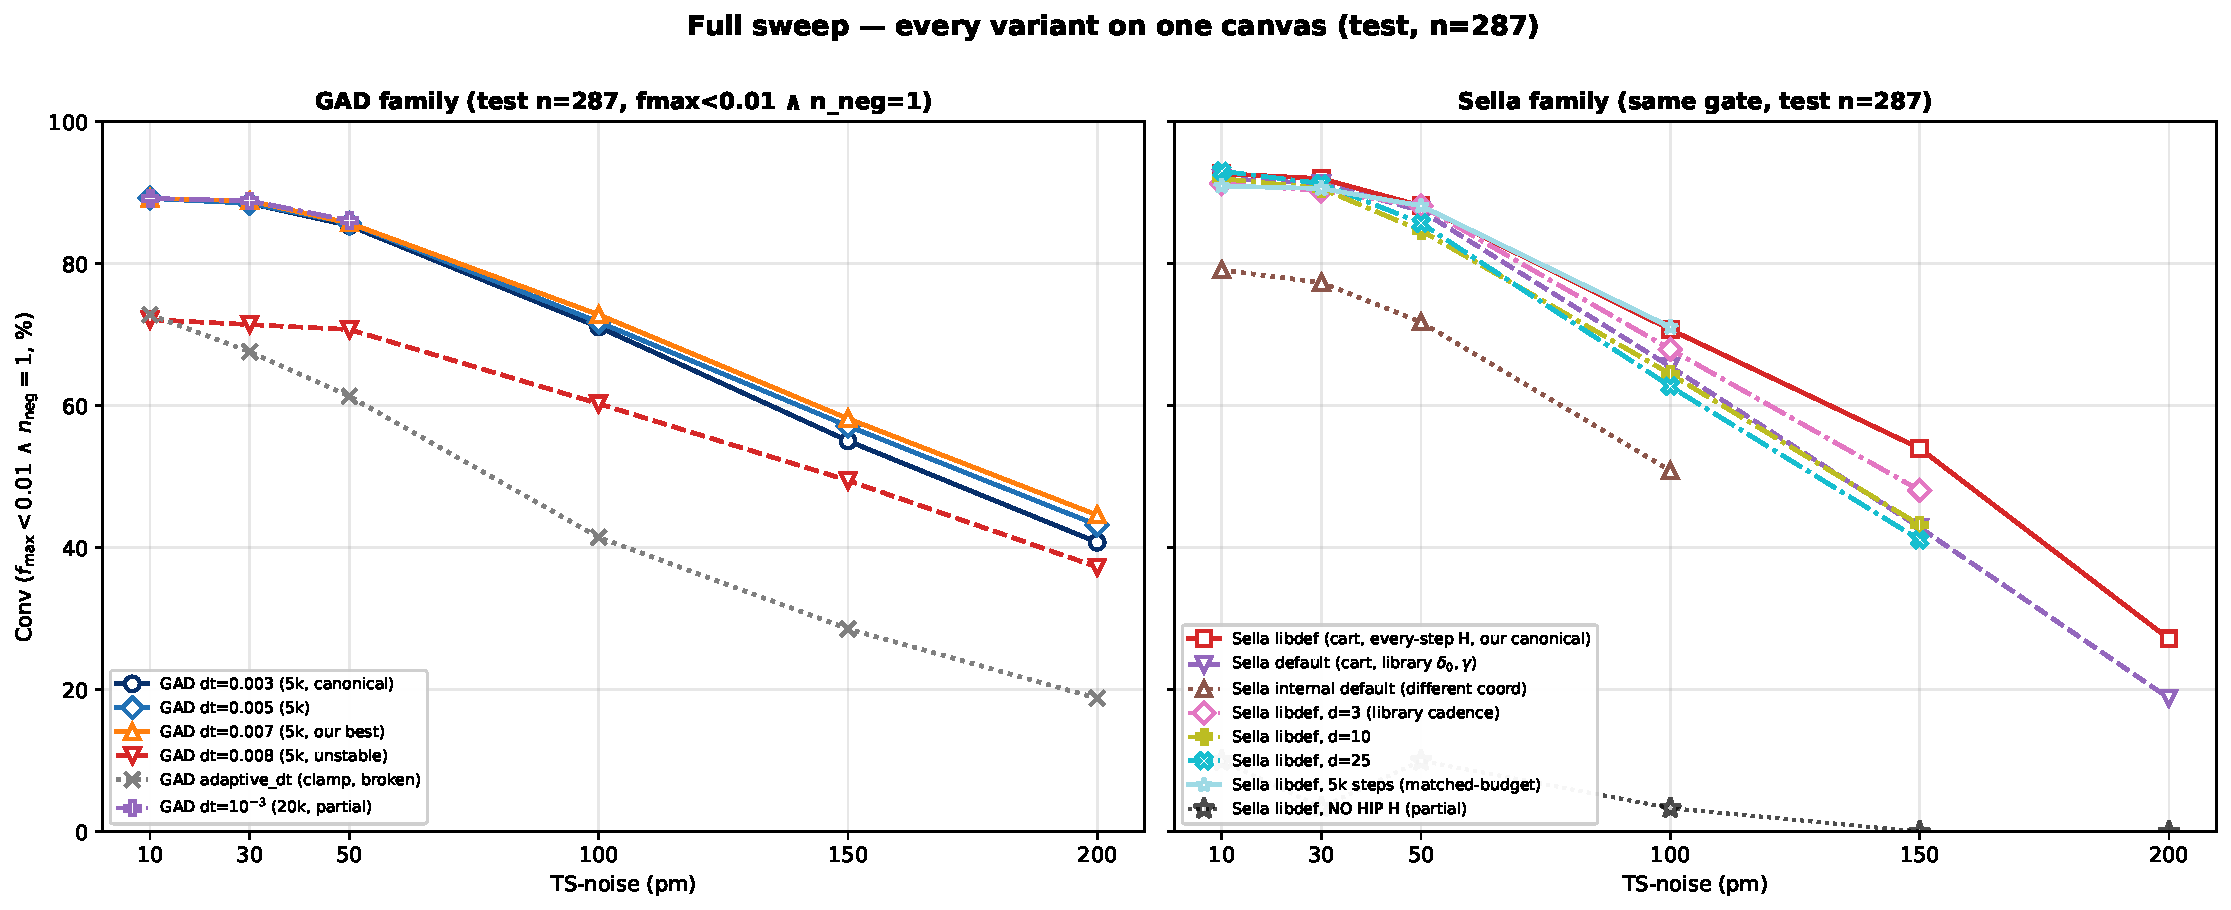
\includegraphics[width=\textwidth]{figures/fig_full_sweep_grid.pdf}
\caption{\textbf{Every method, on one canvas.} Left: GAD family (dt
grid + adaptive + low-dt). Right: Sella family (libdef cart, default
cart, internal coords, Hessian cadences d=3/10/25, matched-budget 5k,
no-Hessian partial). Same criterion ($n_{\text{neg}}{=}1\,\wedge\,f_{\max}{<}0.01$),
test n=287. Color coding: each family stays in one warm/cool palette so
the eye can group them. The ``no HIP H'' (BFGS only) line at the bottom of
the right panel is partial (timed out at 12h with $\sim$5\% conv at every noise).}
\label{fig:full-sweep}
\end{figure}

\begin{figure}[H]
\centering
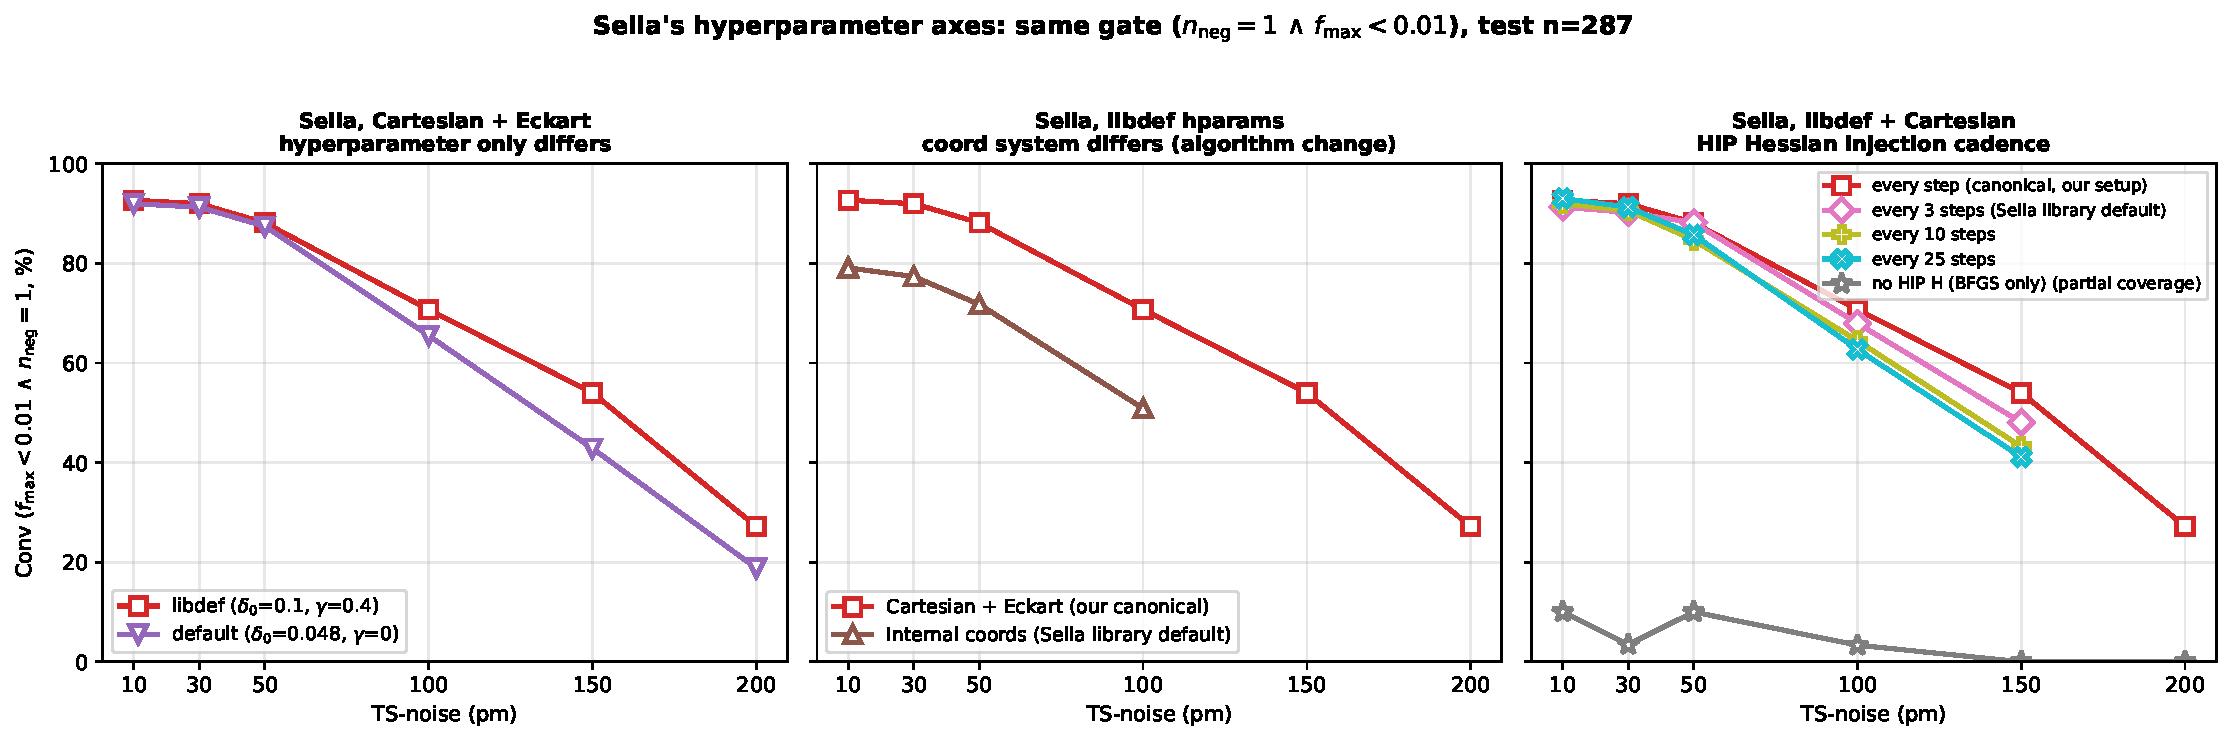
\includegraphics[width=\textwidth]{figures/fig_sella_variants.pdf}
\caption{Sella's three hyperparameter axes, each varied alone.
(A) hyperparameter only ($\delta_0,\gamma$): minor effect. (B) coordinate
system (internal vs Cartesian + Eckart): $\sim$10pp drop at high noise
— this is an algorithm change, not a hparam tweak. (C) HIP H injection
cadence (every 1, 3, 10, 25 steps, vs none): smooth degradation across
$N=1\to 25$ ($-$3 to $-$13pp at 100--150pm), then a cliff to $\sim$5\%
when no Hessian at all. The first 1-of-25 HIP Hessian per chain is what's
load-bearing, not ``every step.''}
\label{fig:sella-variants}
\end{figure}

\begin{figure}[H]
\centering
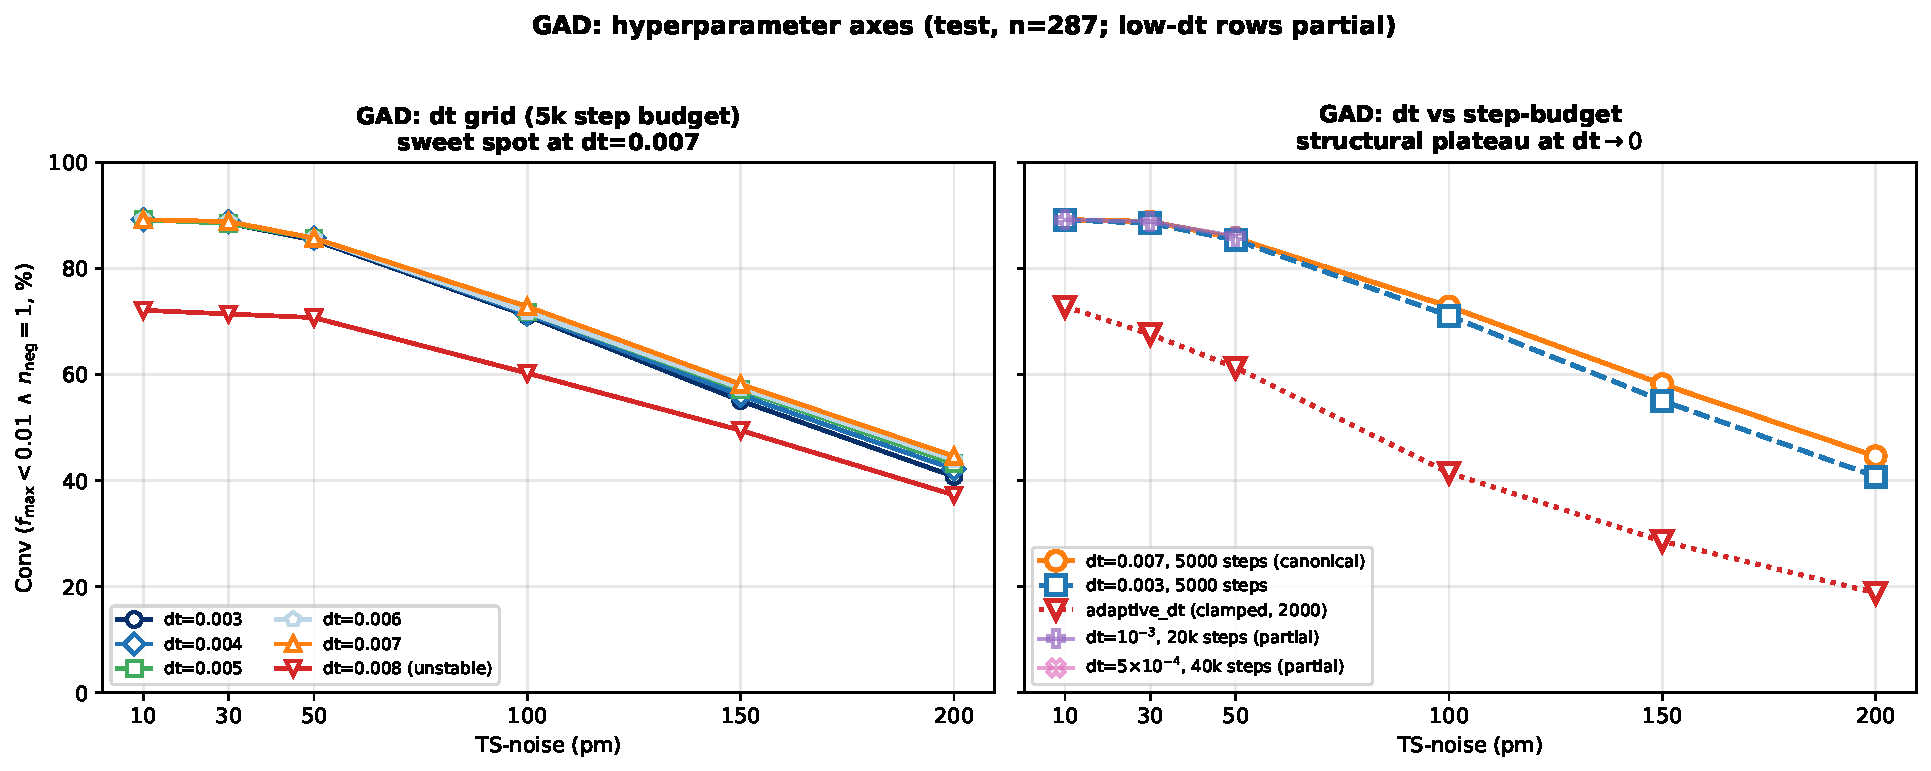
\includegraphics[width=\textwidth]{figures/fig_gad_lineage.pdf}
\caption{GAD's hyperparameter axes. (A) dt grid at fixed 5000-step budget:
monotone improvement from dt=0.003 to dt=0.007; collapse at dt=0.008
from Euler instability ($dt < 2/|\lambda_{\max}|$ is violated by stiff
bond modes). (B) Step-budget tradeoff: dt=0.007/5k beats dt=0.003/5k
beats adaptive\_dt; very-small-dt rows (1e-3, 5e-4 with 20k--40k step
budgets) are partial coverage and confirm the structural plateau —
70$\times$ dt drop changes conv by $\le$5pp.}
\label{fig:gad-lineage}
\end{figure}

\paragraph{IRC scoring sensitivity — headlines robust to knob choices.}
We re-scored the existing IRC parquets at multiple settings to check
robustness:

\begin{center}\small
\begin{tabular}{l|cc|cc|c}
\toprule
                  & \multicolumn{2}{c|}{TOPO @ cutoff=1.2} & \multicolumn{2}{c|}{TOPO @ cutoff=1.3} & gap shift \\
                  & GAD dt=0.007 & Sella libdef & GAD dt=0.007 & Sella libdef & \\
\midrule
200pm             & 52.3 & 31.5 & 53.5 & 32.9 & $-$0.2 \\
\bottomrule
\end{tabular}
\vskip0.4em
\begin{tabular}{l|cc|cc|c}
\toprule
                  & \multicolumn{2}{c|}{RMSD @ thr=0.3 \AA} & \multicolumn{2}{c|}{RMSD @ thr=0.5 \AA} & gap shift \\
                  & GAD dt=0.007 & Sella libdef & GAD dt=0.007 & Sella libdef & \\
\midrule
200pm             & 24.9 & 13.6 & 32.0 & 19.7 & $+$1.0 \\
\bottomrule
\end{tabular}
\end{center}
{\small Numbers denominated by valid-IRC samples (i.e.\ both endpoints
produced); minor difference from headline table which uses $n=287$.
The +21pp GAD-vs-Sella gap at 200pm is preserved within $\pm 1$pp across
both scoring knob variations. Sources:
\texttt{analysis\_2026\_04\_29/irc\_sensitivity.csv} (192 rows for every
method × noise × threshold × cutoff combination), builder
\texttt{scripts/analyze\_irc\_sensitivity.py}.}

\paragraph{How to read the appendix figures.}
\begin{itemize}[leftmargin=1.5em]
\item For the headline narrative, only Fig.~\ref{fig:narrative-irc}
  (Executive Summary) is needed — best-of-each at IRC TOPO.
\item Fig.~\ref{fig:narrative-conv} (Executive Summary) gives the
  raw-conv companion at two thresholds.
\item Fig.~\ref{fig:full-sweep} is the ``everything in one place''
  reference — for reviewers who want to see we tested every variant
  before declaring a winner.
\item Fig.~\ref{fig:sella-variants} \& Fig.~\ref{fig:gad-lineage}
  isolate the hyperparameter axes inside each method family — for
  the discussion of which variants count as ``the same algorithm''
  vs ``a different algorithm''.
\end{itemize}

% =================================================================
\section{NR-polish negative result (added 2026-05-04)}
% =================================================================

\paragraph{What we tried.} A spectral-partitioned Newton--Raphson polish
on top of converged-or-near GAD, hypothesised to break the structural
plateau at $f_{\max}{\approx}0.01$ by switching from explicit Euler
($\dot x = F + 2(F\!\cdot\!v_1)v_1$) to a quasi-second-order step
$\Delta x = -H^{-1} F$ with the unstable mode reflected. Predicted (from
the "GAD plateaus near saddle because $v_1$ noise floor matches $F$
floor" mechanism): NR should drop $f_{\max}$ to $\sim 10^{-5}$ and shrink
final-RMSD to Sella levels.

\paragraph{Configuration.} \texttt{nr\_gad\_polish\_dt007} runner
(\texttt{scripts/method\_single.py}), $dt{=}0.007$, NR phase activates
when $n_{\text{neg}}{=}1$, two thresholds tested: \texttt{loose} (criterion
$f_{\max}{<}10^{-2}$) and \texttt{strict} (criterion $f_{\max}{<}10^{-4}$).
Test split, $n{=}80$ subset, 3000 step budget, 6 noise levels.
SLURM 60314225 (12 cells, all completed in 1.9--4.3 h each).

\paragraph{Result — NR underperforms vanilla GAD.}

\begin{center}\small
\begin{tabular}{l|cccccc}
\toprule
\textit{conv $\equiv n_{\text{neg}}{=}1 \wedge f_{\max}{<}0.01$, percentages.}
& 10 & 30 & 50 & 100 & 150 & 200 \\
\midrule
GAD dt=0.007 (5k, $n{=}287$) — \emph{baseline}      & 89.2 & 88.9 & 85.7 & 72.8 & 58.2 & 44.6 \\
NR-polish loose (3k, $n{=}80$)                       & 65.0 & 48.8 & 46.3 & 37.5 & 30.0 & 30.0 \\
NR-polish strict ($f_{\max}{<}10^{-4}$ criterion, $n{=}80$) & 0.0 &  0.0 &  0.0 &  0.0 &  0.0 &  0.0 \\
\midrule
$\Delta$ (NR-loose -- baseline)                      & $-24.2$ & $-40.1$ & $-39.4$ & $-35.3$ & $-28.2$ & $-14.6$ \\
\bottomrule
\end{tabular}
\vskip0.4em
\textit{NR underperforms by 14–40 pp at every noise. Strict ($f_{\max}{<}10^{-4}$)
fails everywhere; \textbf{not a single sample across all $480$
NR-loose attempts crossed $f_{\max}{<}10^{-3}$} (min observed: $0.0055$).}
\end{center}

\paragraph{Diagnosis.} The minimum $f_{\max}$ achieved across all 480
NR-loose samples was $0.0055$, not the $10^{-5}$ predicted. This rules
out "NR converges deeper than GAD" — NR is doing \emph{worse} than vanilla
GAD even at the loose criterion. Mechanism: the NR step
$\Delta x = -(H + \alpha v_1 v_1^\top)^{-1} F$ takes \emph{large} jumps
near the saddle where $H$ is near-singular along the $v_1$ direction.
Those jumps overshoot the saddle basin, requiring GAD to re-approach.
The flip-flop never settles. Final $f_{\max}$ averages 0.21--0.72 (vs
GAD baseline 0.024--0.27).

\paragraph{Average $f_{\max}$ at termination.}
\begin{center}\small
\begin{tabular}{l|cccccc}
\toprule
& 10 & 30 & 50 & 100 & 150 & 200 \\
\midrule
GAD dt=0.007 (5k) avg $f_{\max}$ at end  & 0.024 & 0.025 & 0.050 & 0.125 & 0.199 & 0.269 \\
NR-polish loose avg $f_{\max}$ at end    & 0.21 & 0.41 & 0.36 & 0.72 & 0.48 & 0.62 \\
\midrule
\multicolumn{7}{l}{\textit{NR-loose ends at 4–10$\times$ \emph{higher} $f_{\max}$ than vanilla GAD.}} \\
\bottomrule
\end{tabular}
\end{center}

\paragraph{Implication for the paper.} NR-GAD polish (the canonical
"level 4" feature in the bottom-up plan) is \emph{not} a path to tighter
convergence as currently implemented. The structural plateau at
$f_{\max} \approx 0.01$ stays. Two paths forward, neither fast:
\begin{enumerate}[leftmargin=1.5em]
\item Trust-region NR (cap $\|\Delta x\|$ by some radius $\delta$), so
  the polish phase doesn't overshoot. Effectively re-implementing
  Sella's RFO logic on top of GAD.
\item Skip NR; treat the plateau as physical and accept GAD's
  $f_{\max}{\sim}10^{-2}$ floor. \emph{This is what the paper's headline
  result already does — IRC validation works at the loose criterion.}
\end{enumerate}

\paragraph{Sources.}
\texttt{runs/test\_nrpolish/nr\_gad\_polish\_dt007\_\{loose,strict\}/summary\_*.parquet}
(960 samples total). SLURM logs:
\texttt{logs/testnrpolish\_60314225\_\{0..11\}.\{out,err\}}.

\newpage
% =================================================================
\section{Pending experiments (will append once data lands)}
% =================================================================

\begin{itemize}[leftmargin=1.5em]
\item \textbf{From reactants} (60110201, $\sim$10h remaining): GAD vs Sella starting from $\textbf{R}$ minimum. Partial: GAD$\approx$50--60\%, Sella$\approx$80--87\% on raw conv (\texttt{logs/testreact\_60110201\_*.out}). Awaiting IRC validation for ``intended'' interpretation.
\item \textbf{IRC TOPO validation rerun} (60146557): previous 60110465 had a \texttt{split="train"} bug; smoke 60145419 verified the fix (1/5 RMSD-INTENDED, 4/5 TOPO-INTENDED). Full 36-cell rerun queued.
\item \textbf{Low-dt diagnostic} (60110297): partial data already shows plateau is structural (see §Low-dt section above).
\item \textbf{Sella Hessian-frequency sweep} (60147671): \texttt{diag\_every}$\in\{3,5,10,25\}$ on libdef config, 6 noise levels. Fills the gap between ``every step'' and ``never'' Hessian-injection cadences.
\item \textbf{NR-GAD polish} (60151717 timed out, relaunched 60314225 with $n{=}80, 3000$ steps, 18h time):
  \emph{landed 2026-05-04 — predicted-help-but-didn't.}
  See §"NR-polish negative result" below.
\item \textbf{Midpoint single-ended} (60153126): GAD dt=0.003/0.007 + Sella libdef + Sella internal default, all from R+P linear midpoint at 0pm noise. Adds the ``geodesic midpoint'' starting condition the user asked for.
\item \textbf{Huge-noise probe} (60154004): noise $\in\{300, 500, 1000, 2000\}$ pm $\times$ 4 methods (GAD dt=0.003/0.007, Sella libdef-2k, Sella libdef-5k step budget) $\times$ n=50. Tests: Sella wrong-saddle failure at huge noise, Sella step-budget question (does 5k vs 2k help?), HIP Hessian quality at huge displacement, GAD/HIP robustness limits.
\end{itemize}

\newpage
% =================================================================
\section{Data locations}
% =================================================================

See \texttt{analysis\_2026\_04\_29/DATA\_INDEX.md} for full schemas and
example DuckDB queries against every CSV/parquet listed below.

\begin{center}\small
\begin{tabular}{ll}
\toprule
Artifact & Path / source \\
\midrule
GAD test (3 methods, 2000 steps)  & \texttt{runs/test\_set/gad\_*} \\
GAD dt grid (6 dts, 5000 steps)   & \texttt{runs/test\_dtgrid/gad\_dt00\{3..8\}\_fmax} \\
GAD low-dt (3 dts, scaled budget) & \texttt{runs/test\_lowdt/gad\_dt\{001,0005,0001\}\_fmax} \\
Sella test (3 configs)            & \texttt{runs/test\_set/sella\_*} \\
Sella no-Hessian (timed out)      & \texttt{logs/testsellanohess\_60110188\_*.out} (parsed) \\
Sella recovery (high-noise)       & \texttt{runs/test\_set/sella\_*} (4 cells), \texttt{logs/testsellarec\_*} \\
Sella Hessian-freq sweep          & \texttt{runs/test\_hessfreq/sella\_carteck\_libdef\_d\{3,5,10,25\}/} \\
From reactants (4 methods)        & \texttt{runs/test\_reactant/*}, \texttt{logs/testreact\_60110201\_*.out} \\
IRC validation (rerun, in flight) & \texttt{runs/test\_irc/*}, log \texttt{logs/testirc\_60146557\_*.out} \\
Threshold sweep CSV               & \texttt{analysis\_2026\_04\_29/threshold\_sweep.csv} \\
Saddle-quality table              & \texttt{analysis\_2026\_04\_29/saddle\_quality\_table.md} \\
Test summary CSV                  & \texttt{analysis\_2026\_04\_29/test\_summary\_full.csv} \\
GAD RMSD-to-TS                    & \texttt{analysis\_2026\_04\_29/gad\_test\_rmsd.csv} \\
Sella nohess (parsed)             & \texttt{analysis\_2026\_04\_29/sella\_nohess\_partial.csv} \\
Findings narrative                & \texttt{analysis\_2026\_04\_29/FINDINGS.md} \\
Figures                           & \texttt{figures/fig\_test\_*.pdf}, \texttt{figures/fig\_rmsd\_*.pdf} \\
Builders                          & \texttt{scripts/analyze\_threshold\_sweep.py}, \texttt{scripts/figures\_test\_2026\_04\_29.py}, \texttt{scripts/analyze\_rmsd\_\{gad,bimodal\}.py}, \texttt{scripts/parse\_nohess\_logs.py} \\
This report                       & \texttt{IRC\_TEST\_2026-04-29.tex/pdf} \\
Live status                       & \texttt{LIVE\_STATUS.md} (resume-after-compaction reference) \\
\bottomrule
\end{tabular}
\end{center}

\end{document}
